% describe user interface
% \section{Interface with the Oracle}
\label{ch:interface-oracle}

In this chapter, we describe one implementation of the Oracle. In \autoref{alg:newcandidate}, the candidate is obtained as $C = \mathcal{O}(H_i^{+}, H_i^{-})$. The Oracle $\mathcal{O}$ considers two sets of concrete heaps $H_i^{+}$ and $H_i^{-}$, and returns a candidate pattern $C$ which is then evaluated. After the evaluation, it is either accepted, or needs to be further refined, in which case $H_i^{+}$ or $H_i^{-}$ are updated, and a new query is submitted to the Oracle. This process repeats until a suitable candidate is found for the current vertex in the program unwinding.

\section{Human as an Oracle}
Human beings are good at finding patterns in several types of spatial data. This fact has been utilized for crowdsourcing the harder parts of several difficult technical problems (cite away). The important challenges are to identify steps in the problem where human insight is critical, find ways to transform these steps into tasks that non-expert humans can perform, and combine the results to resolve those steps in the solution. In our problem of verifying heap-manipulating programs, the goal of the Oracle is to provide heap patterns that can be used to generate interpolants, which are then used for verification. Finding these interpolants automatically is a difficult step in program verification, while checking a provided interpolant for correctness is relatively easier to automate. Later in \autoref{sec:expressiveness-of-heap-patterns} and \autoref{sec:understandability-of-interface}, we discuss more elaborately how our heap pattern language and interface fare as tools to input human insight.

\section{Web Interface}
\label{sec:web-interface}
As a practical demonstration of the Oracle, we designed a web interface that shows examples of concrete heap to a human user. The interface allows them to construct a pattern graph using a graphical interface. The pattern graph should be such that it covers all positive examples, but doesn't cover any negative example.

Our graphical interface, created using D3 \cite{d3js} is a way for our Oracle (human) to interact with the \verifier algorithm. The interface is designed to make it simple to input heap pattern graphs and receive quick feedback about the correctness the pattern graph. Pattern graphs have several characteristics, as described in \autoref{defn:pattern}, and it can be challenging and overwhelming for the user to input a graph that generalizes enough, but not so much that it becomes useless for the underlying verification algorithm. Since our Oracles are humans, it is crucial that we create the best experience for them to input information to the prover.

Later, we describe in \autoref{sec:who-are-the-users} what kind of background we expect from our users. One of our goals was to design an interface that would not need expertise in software verification. This means that the user input language has to be such that it not only works well with our heap pattern formalism, but also avoids the need for users to interact with the formalism directly. Since heaps and heap patterns are essentially graphs, we decided it was reasonable to represent these as visual graphs, and also allow users to ``draw'' graphs while getting instant feedback. We decided to use force-directed graphs in D3 for our implementation.

\subsection{Force-Directed Graphs in D3.js}
Before moving on with the description of our implementation, we briefly describe the Javascript library D3 that we used to build our heap pattern web interface. D3 allows to bind data to a Document Object Model (DOM), and then apply data-driven transformations to the document. For example, D3 can be used to generate an HTML table from an array of numbers. Or, the same data can be used to create an interactive SVG bar chart with smooth transitions and interaction. The key problem solved by D3 is efficient manipulation of documents based on data. D3 is capable of supporting large datasets, and a wide variety of dynamic behaviors and interactions.

Force-directed graph drawing algorithms \cite{eades84, fruchterman91} are a class of algorithms for drawing graphs in an aesthetically pleasing way. Their purpose is to position the nodes of a graph in two or three-dimensional space so that all edges are of more or less equal length and there are as few crossing edges as possible, by assigning forces among the set of edges and the set of nodes, based on their relative positions, and then using these forces either to simulate the motion of the edges and nodes or to minimize their energy. This is exactly like a simulation of an actual physical system in space. It is possible to define different ``forces'' such as those arising from gravity, electrical charges, elasticity, etc., and assign them to edges, nodes, and other components of the graph. The algorithm combines all these forces together, trying to reach a stable state. The key is to carefully calibrate the forces so that the resulting graph visualization is suitable. There are several ways force-directed graphs can be modeled, but we used D3's inbuilt model, that makes it really easy to create a simple force-directed graph. It works by defining nodes and links, and appends HTML objects to them. As the nodes and links interact to reach stable state, the HTML objects move along, making the visualization a graph built on top of an underlying force-directed graph drawing algorithm.

\subsubsection{Advantages and Disadvantages of Force-directed graphs}
We chose force-directed graphs because they are designed for drawing graphs in an aesthetically pleasing way, especially ones for which structure is unknown beforehand. Our positive and negative heap examples are often large and have diverse structures, and it's not trivial to have a pre-defined way of drawing them. Force-directed drawing algorithms take care of this, and are highly configurable. Our earlier familiarity with them was also a factor in the choice.

The one major disadvantage is that the spatial relationships of the original nodes change when nodes or edges are modified. Essentially, a local modification can cause a global change of layout, making it harder for users to remember how the same example changed over time. In the future, it will certainly be worthwhile to explore more graph-drawing algorithms.

\subsection{Interface for Drawing Pattern Graphs}

The basic interface for drawing heap graphs is shown in \autoref{fig:basic-graph-interface}. This is what it would look like on starting the visualization. The graph on the right is a force-directed graph representing the current heap pattern. Nodes are represented by circles, and edges by arrows connecting the circles. Arrows are directed, and for simplicity we assume that each node has outgoing fields of only one type. For instance, a data structure with a $next$ pointer would fit this case very well. All nodes and edges are interactive, and allow for different actions to express a rich language of heap patterns.

The form on the left allows the user to interact with the graph and set values for the heap and predicate labelings. The predicates and heap variables have been inferred by the program analysis already.

\begin{ex}
\label{ex:basic-graph-interface}
In \autoref{fig:basic-graph-interface}, the user can select a node (say $n$) by clicking it, pick a predicate (say $p1$), pick a value (say $\true$), and click on "Set value". This would set the value for the the pair of selected node and predicate to $\true$. In our heap pattern formalism from \autoref{defn:pattern}, this would amount to setting $\predlblnm(n, p1) = \true$.

Similarly, picking a heap variable (say $x$) and setting a value (say $\maybe$) for it using the form would amount to setting $\varlblnm(n,x) = \maybe$ for the selected node $n$.
\end{ex}

% Figure with the basic pattern graph interface
\begin{figure}
  \centering
  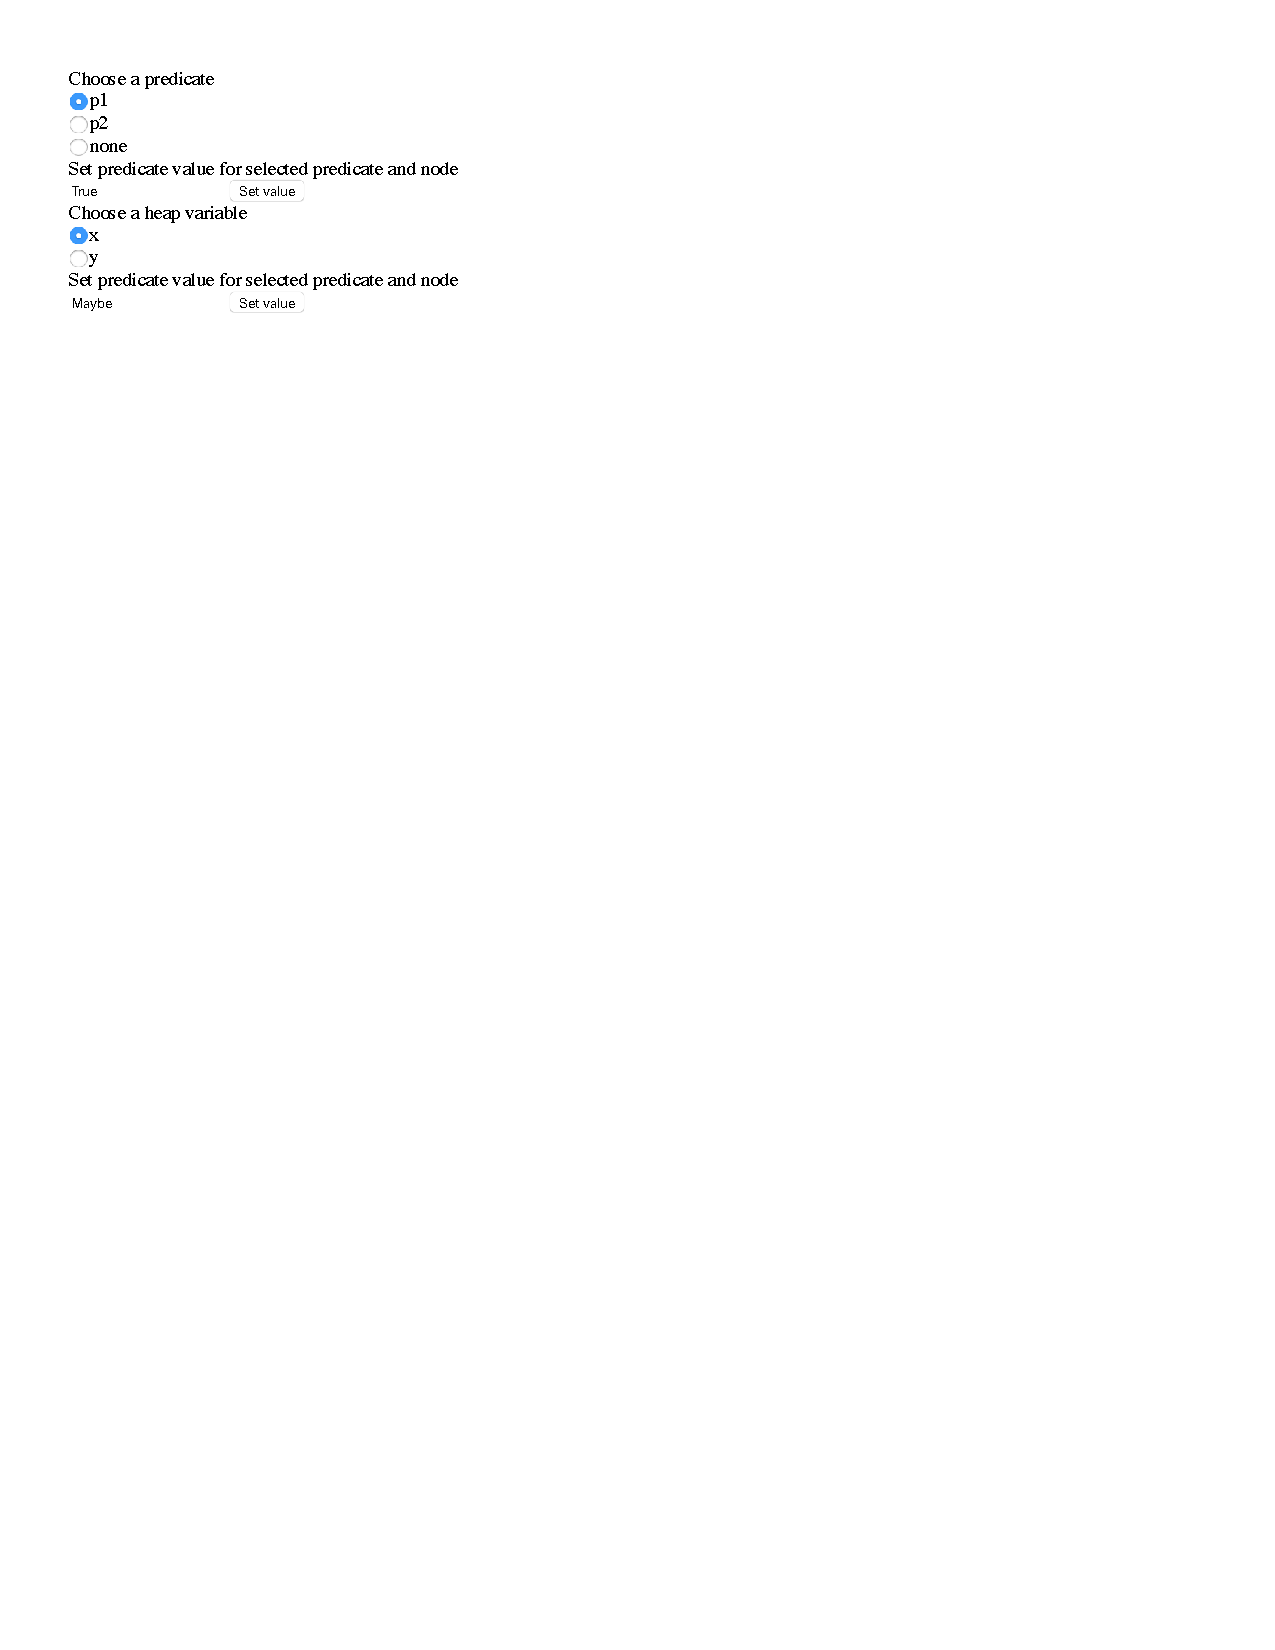
\includegraphics[width=7cm]{fig/predicate-heapvar-val.pdf}
  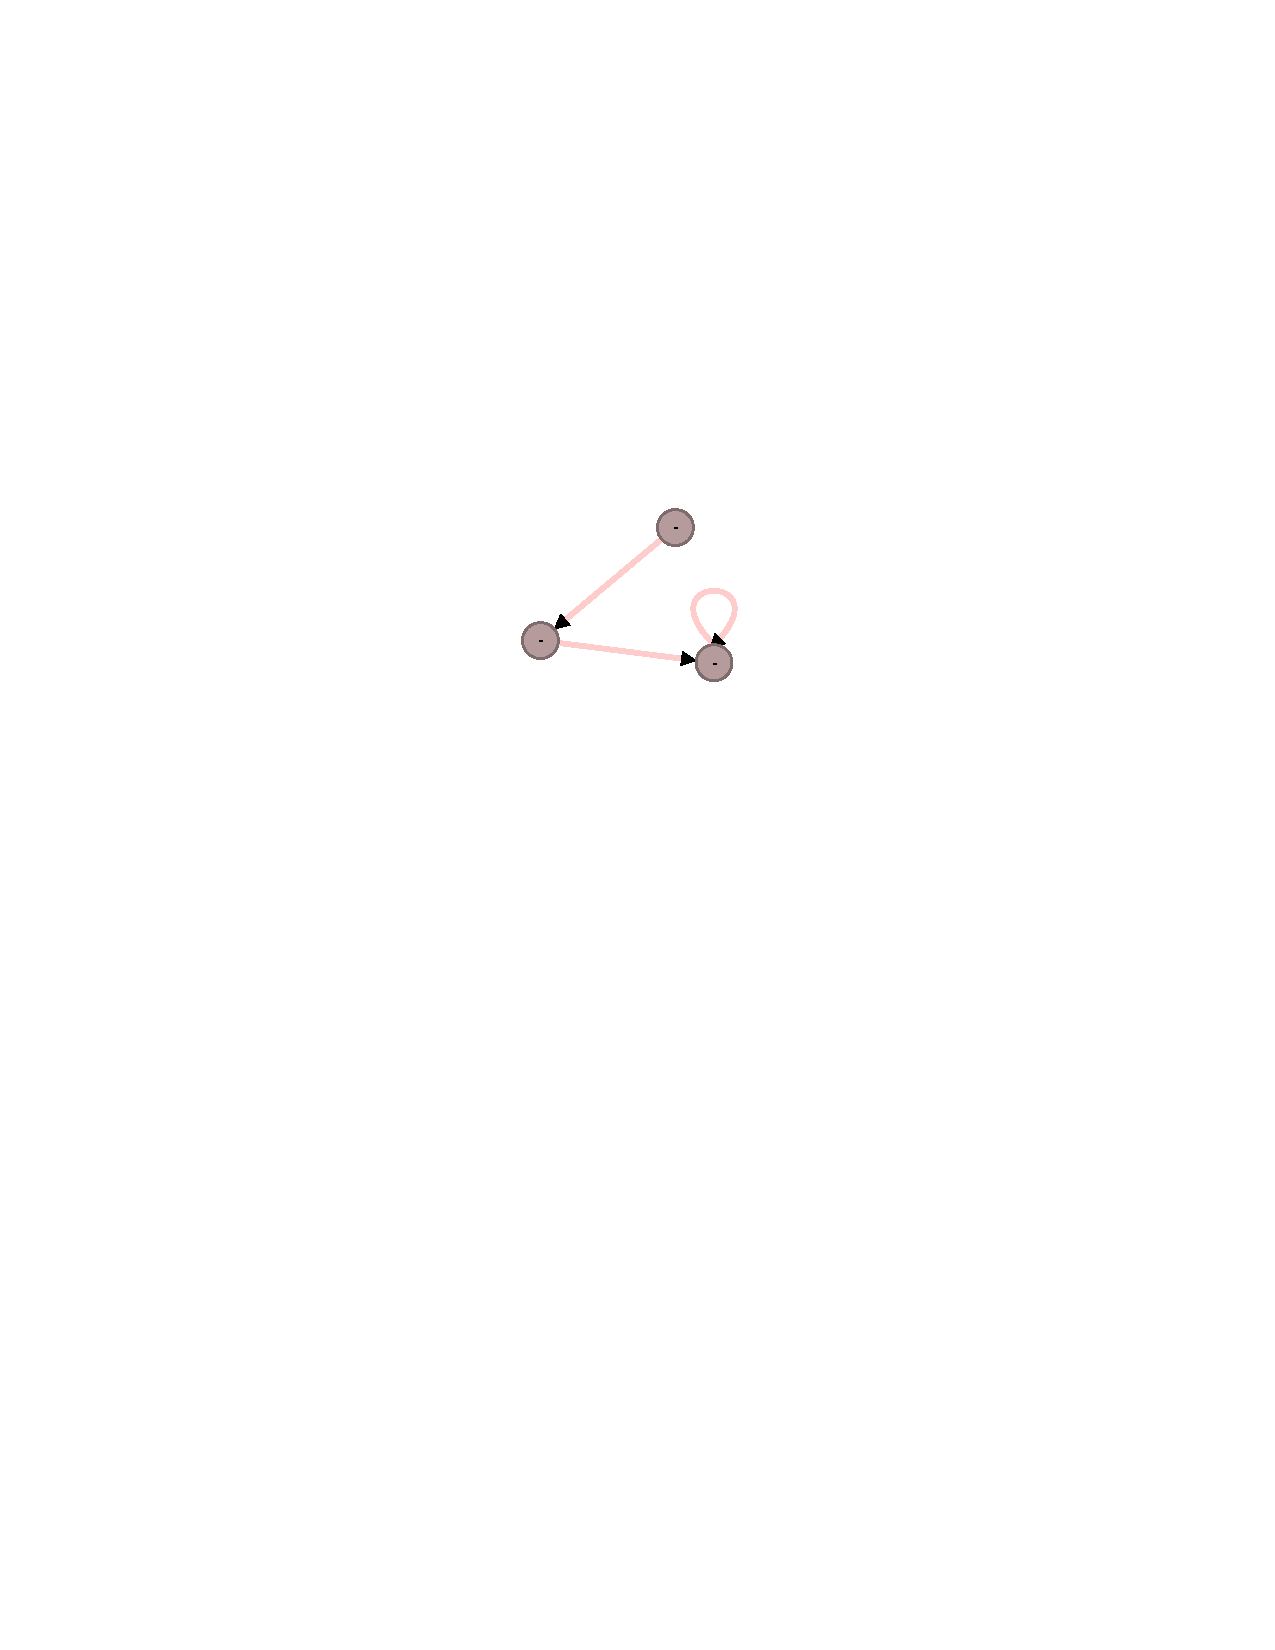
\includegraphics[width=7cm]{fig/basic-graph.pdf}
  \caption{A simple interface to allow the user to graphically draw the heap pattern, and pick values for the predicate and heap variable labeling. The predicates and heap variables have been chosen and populated from a prior analysis. Nodes are represented by circles, and edges as arrows between nodes.
  }
  \label{fig:basic-graph-interface}
\end{figure}

\subsubsection{Who are the Users?}
\label{sec:who-are-the-users}
Our system involves human users, so it is important to describe suitable candidates who will be able to use our system. We believe that a basic understanding of graphs or transition systems should be sufficient, and in fact very helpful in fully grasping what we expect from the user. This means that someone with an undergraduate degree in Computer Science or Mathematics, or indeed anyone who has learned about graphs and state transition systems would be a suitable user. A background in formal methods or verification is not required.

We now dive deeper into all the features provided by the interface, and the user can easily provide a graph pattern matching the formalism described in \autoref{defn:pattern}. One of the important goals of this design is that the user should not have to understand or deal with the formalism itself, but just figures, so that someone with no knowledge of software verification or heap modeling can perform the function of an Oracle.

A heap pattern is a labeled graph represented by the tuple $(\nodesnm, \varlblnm, \predlblnm, \edgesnm, \sigma)$, respectively containing the set of nodes, heap variable labeling, predicate labeling, edges, and summary function. Our interface allows the user to modify the values of each of these attributes of the pattern. We now describe each of these in greater detail.

\subsubsection{Modifying Nodes}
Interacting with nodes allows the user to modify the existing set of nodes. The following actions are available:
\begin{itemize}
  \item Click anywhere on empty space to create a new node.
  \item Click on an existing node to select (or unselect) it. Selected nodes appear a lighter shade than unselected nodes. Only up to one node can be selected at a time.
  \item Press the backspace key after selecting a node to delete it. This deletes all edges and resets other attributes relevant to the node.
\end{itemize}

\autoref{fig:modifying-nodes} illustrates the above points clearly.

% Figure illustrating node modification.
\begin{figure}
  \centering
  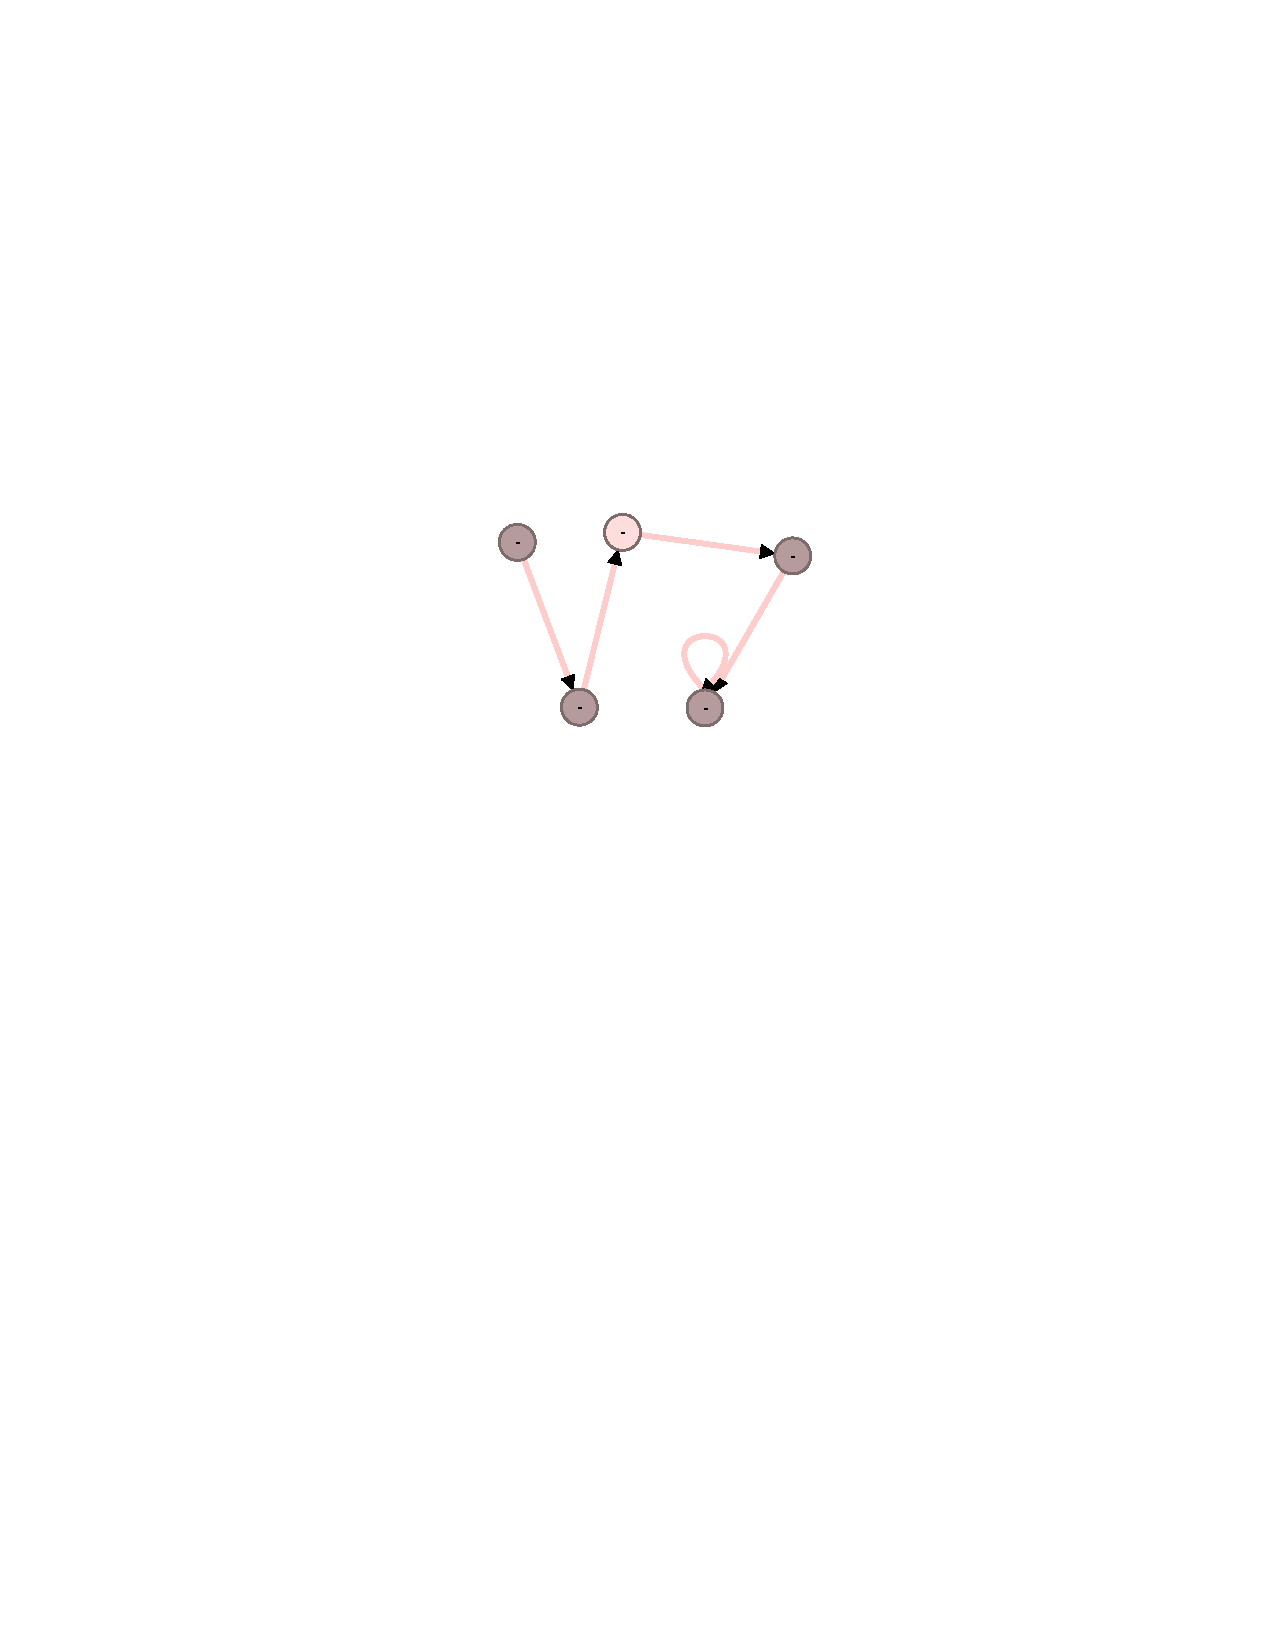
\includegraphics[width=7cm]{fig/nodes-original.pdf}
  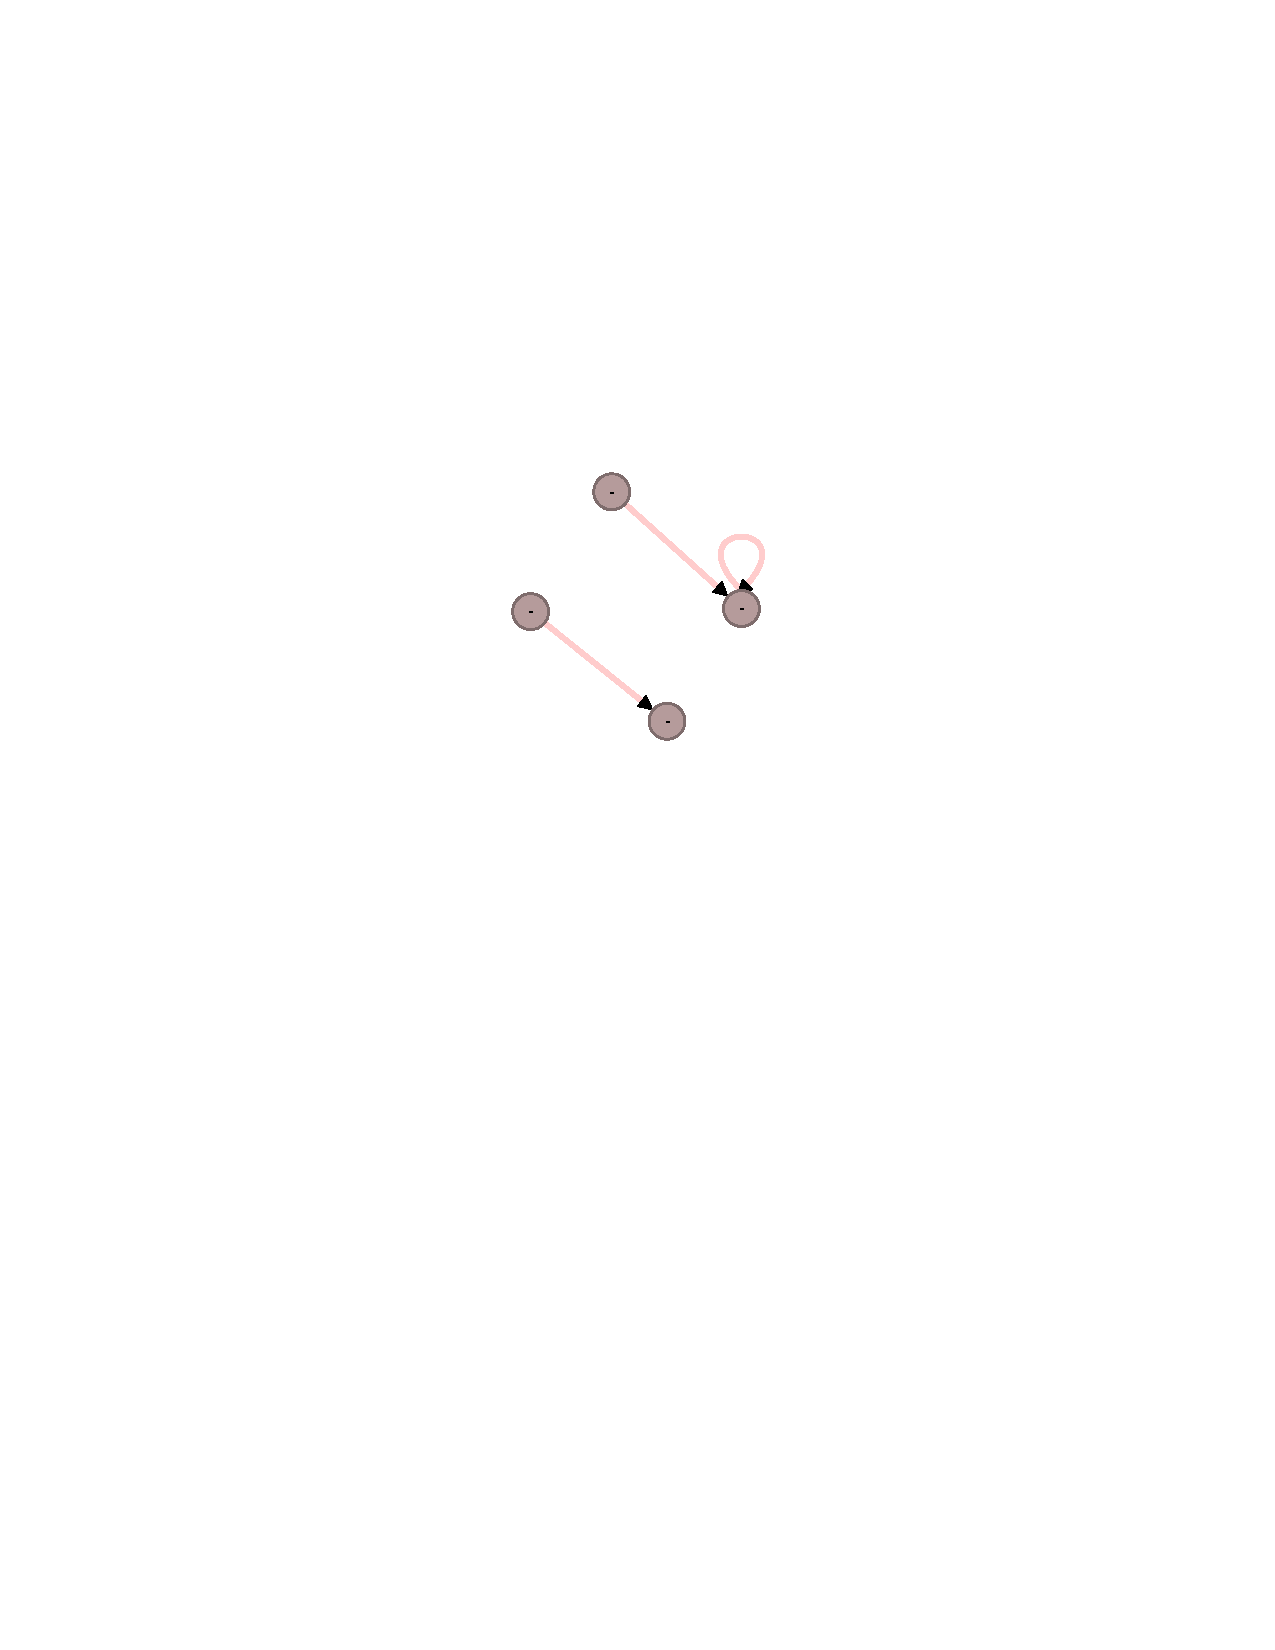
\includegraphics[width=7cm]{fig/nodes-changed.pdf}
  \caption{On the left, the original pattern graph has five nodes, with the middle node selected (indicated by the different color). Pressing the backspace key deletes the node, resulting in the graph on the right.
  }
  \label{fig:modifying-nodes}
\end{figure}

\subsubsection{Modifying the Heap Variable Labeling}
We briefly described the mechanism for updating the heap variable labeling in \autoref{ex:basic-graph-interface}. The interface itself is simple, as shown in \autoref{fig:basic-graph-interface}. In addition, there are some features that make it simpler to keep track of assignments, while preventing user mistakes.

The heap variable labeling is a map $\varlblnm: \nodesnm \times \heapvars \to \threevals$, meaning that each pair of node and heap variable must have a value. To indicate the current assignment, we label the node accordingly. For instance, if the current heap variables are $x, y, z$, and for node $n$, the values of $\varlblnm$ are $\varlblnm(n, x) = \maybe, \varlblnm(n, y) = \true, \varlblnm(n, z) = \false$, then the node will get labeled as $x?y$. The $?$ indicates a $\maybe$ value, the absence of a $?$ indicates $\true$, and absence of the variable altogether indicates $\false$. This keeps the labeling simple, preventing clutter from a large number of $\false$ values, while still making it simple to get a quick idea of the current assignments. Finally, a node with no variable assignments will simply have the label $-$.

We note that $\varlblnm$ is not allowed to have arbitrary assignments. For instance, a variable $x$ cannot be $\true$ for more than one node at the same time. Our interface takes care of such constraints as follows:

\begin{itemize}
  \item Setting a variable to $\true$ for a node sets it to $\false$ for all other nodes automatically.
  \item Setting a variable to $\maybe$ for a node sets it to $\maybe$ for the node where it might currently be $\true$.
\end{itemize}

\autoref{fig:modifying-heap-vars} further illustrates how heap variable labeling works.

% Figure illustrating heap var labeling modification.
\begin{figure}
  \centering
  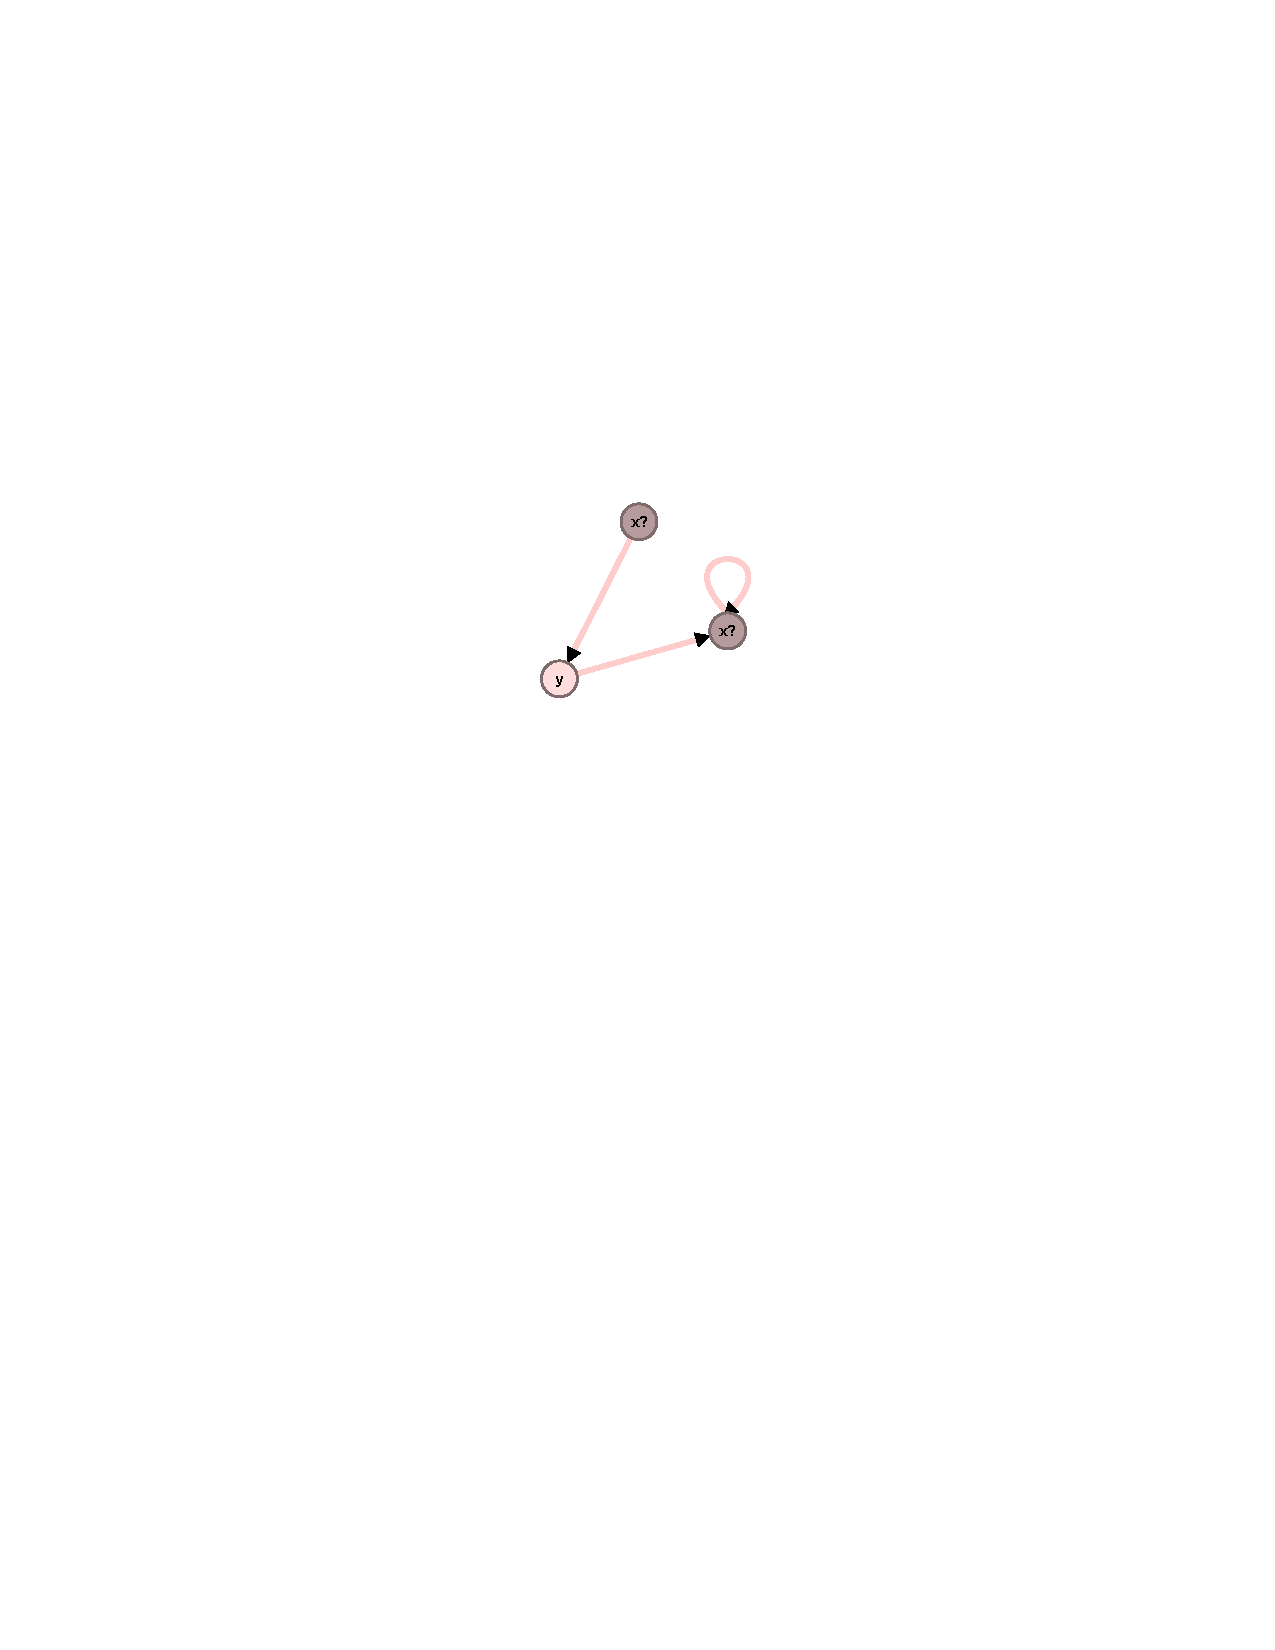
\includegraphics[width=5cm]{fig/heap-var-labeling.pdf}
  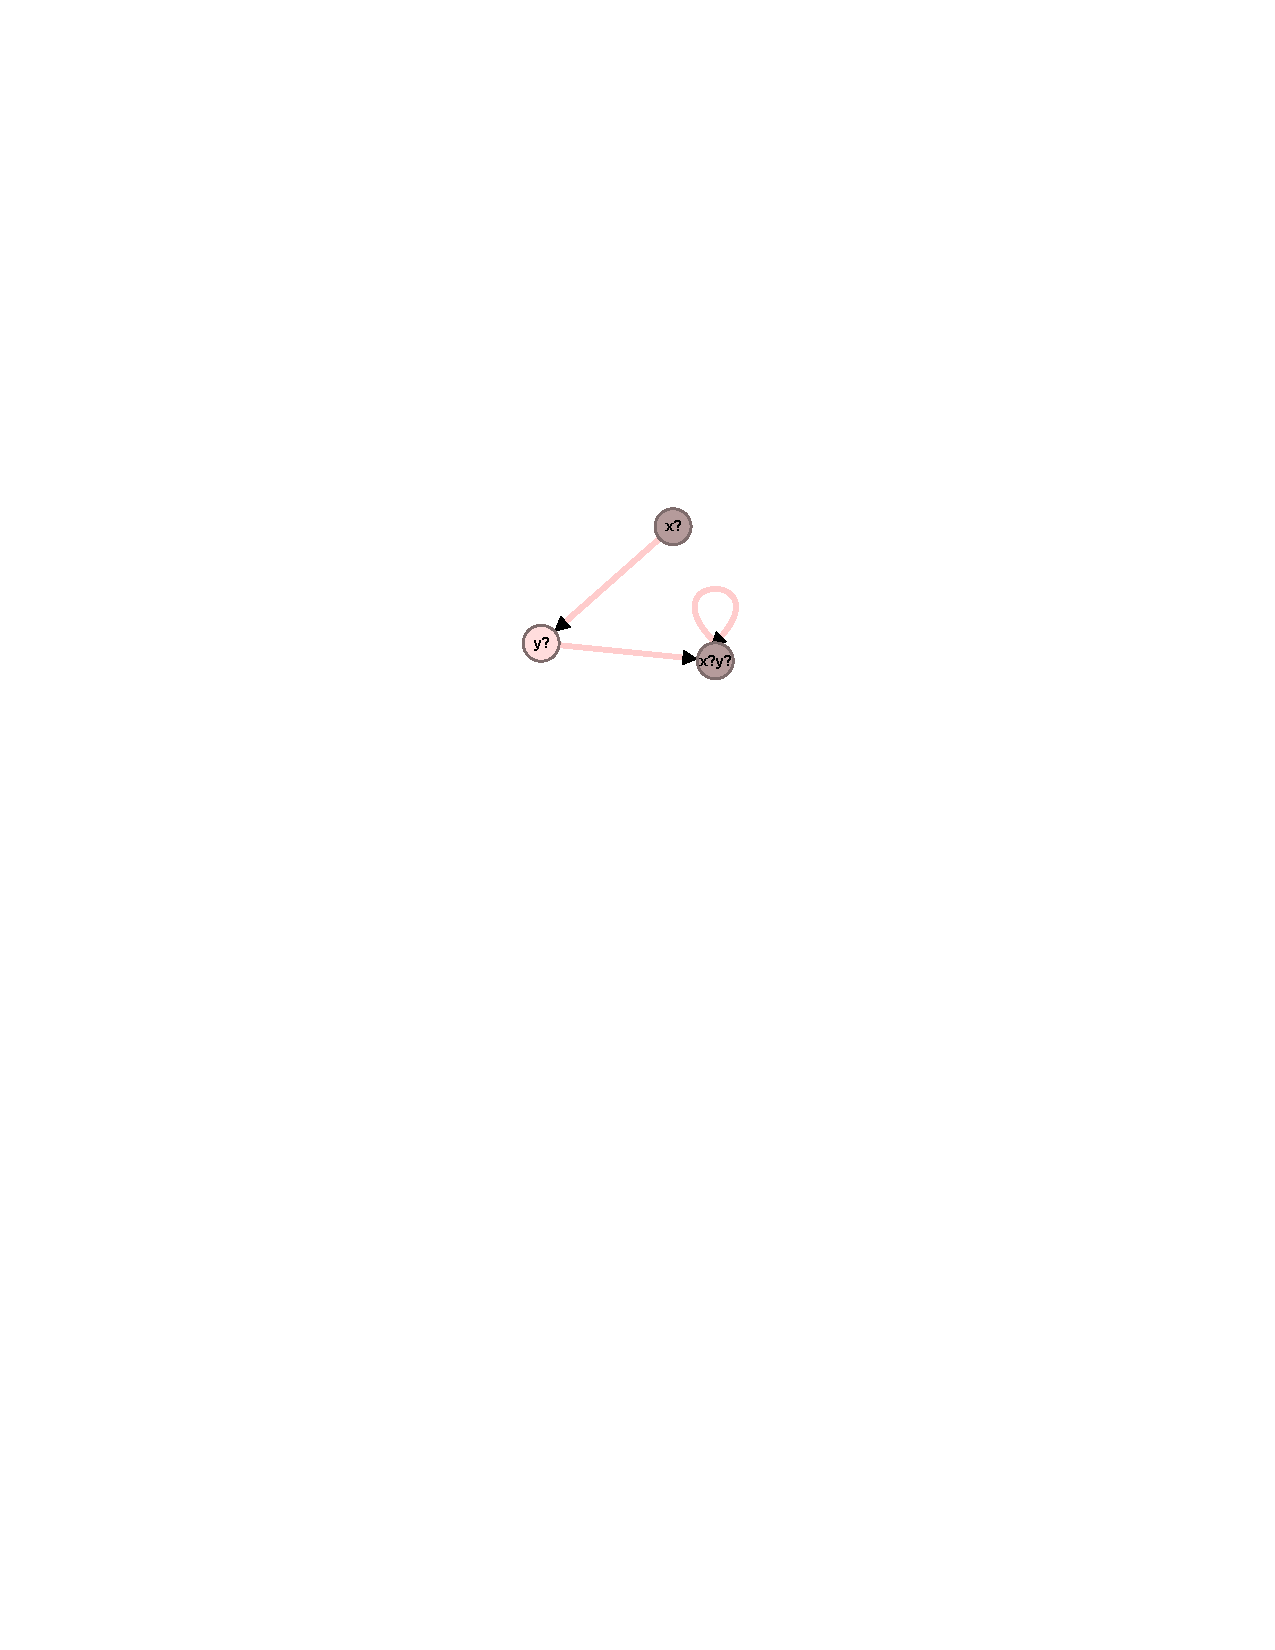
\includegraphics[width=5cm]{fig/heap-var-labeling-2.pdf}
  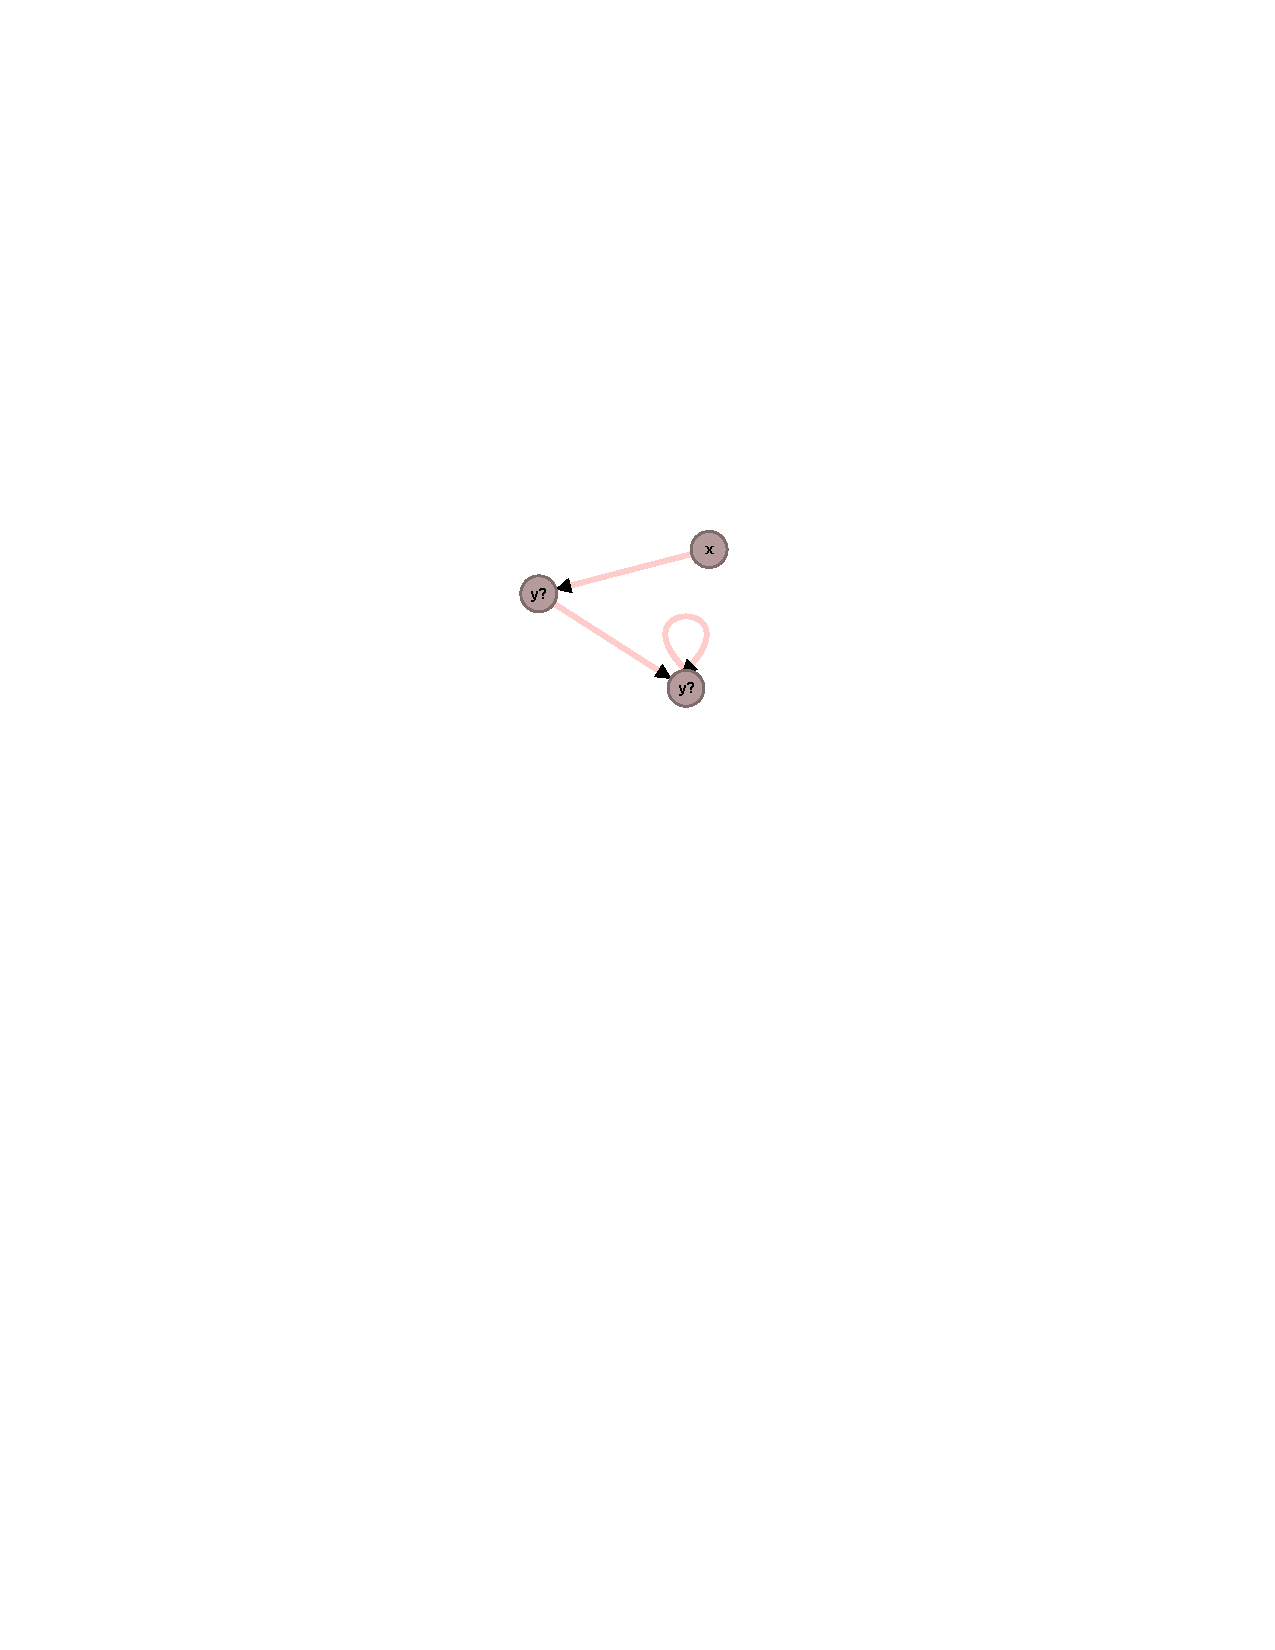
\includegraphics[width=5cm]{fig/heap-var-labeling-3.pdf}
  \caption{The first pattern on the left shows an existing heap variable labeling. We then set the value for $y$ and the node with the self-loop to $\maybe$, which automatically sets the value for $y$ and the selected node to $\maybe$, even though it was $\true$ earlier. Furthermore, in the second pattern, when $x$ is set to $\true$ for the starting node, the value of $x$ is unset for the node with the self-loop.
  }
  \label{fig:modifying-heap-vars}
\end{figure}

\subsubsection{Modifying the Predicate Variable Labeling}
We briefly described the mechanism for updating the predicate variable labeling in \autoref{ex:basic-graph-interface}. The interface itself is simple, as shown in \autoref{fig:basic-graph-interface}. In addition, there are some features that make it simpler to keep track of assignments.

The predicate variable labeling is a map $\predlblnm: \nodesnm \times \predvars \to \threevals$, meaning that each pair of node and predicate variable must have a value. To indicate the current assignment, we use color coding for the nodes - $\predlblnm(n, p) = \true$ imples green, $\predlblnm(n, p) = \false$ imples red, and $\predlblnm(n, p) = \maybe$ implies light pink. Notice that the pattern graph can have multiple predicates available at a time, so the color coding depends on a predicate that is ``live'' at a given time. Predicates can be made live by simply selecting them in the interface shown in \autoref{fig:basic-graph-interface}.

% Figure illustrating pred var modification.
\begin{figure}
  \centering
  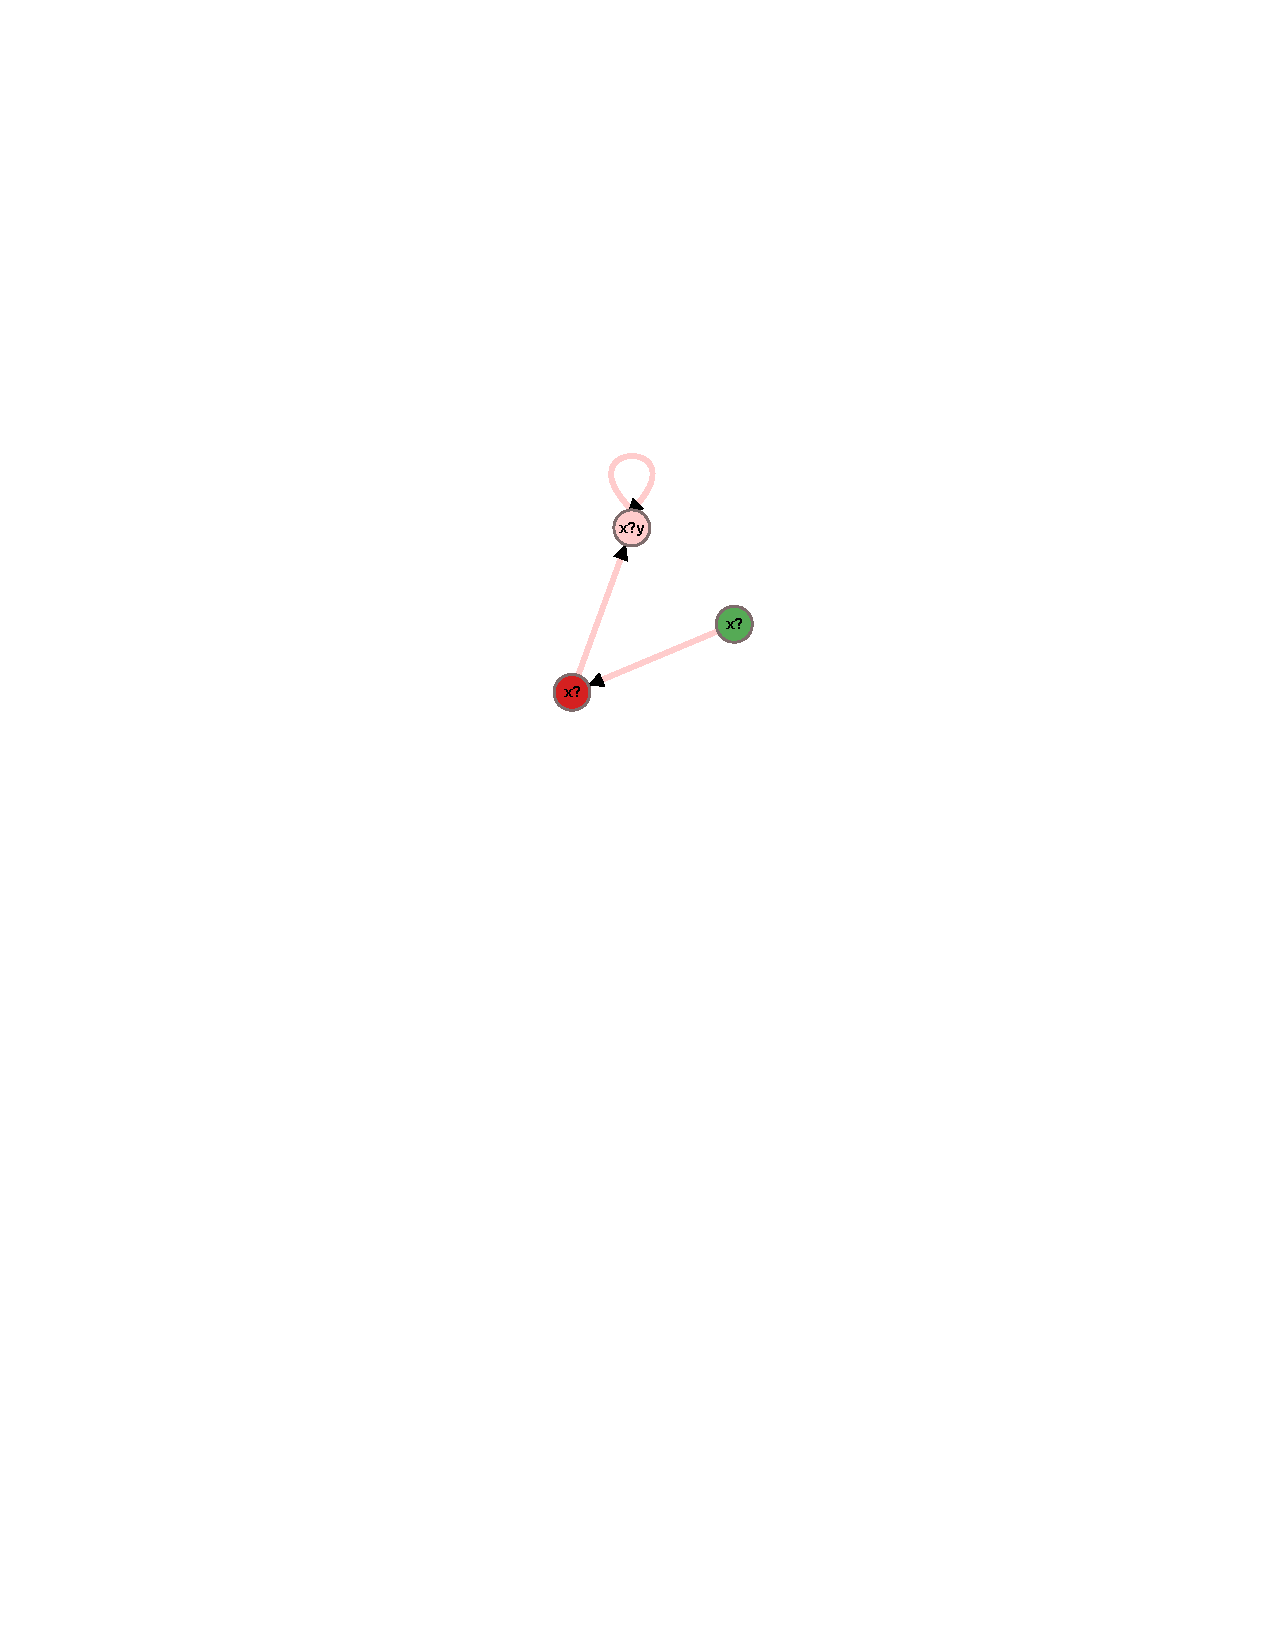
\includegraphics[width=7cm]{fig/predvar.pdf}
  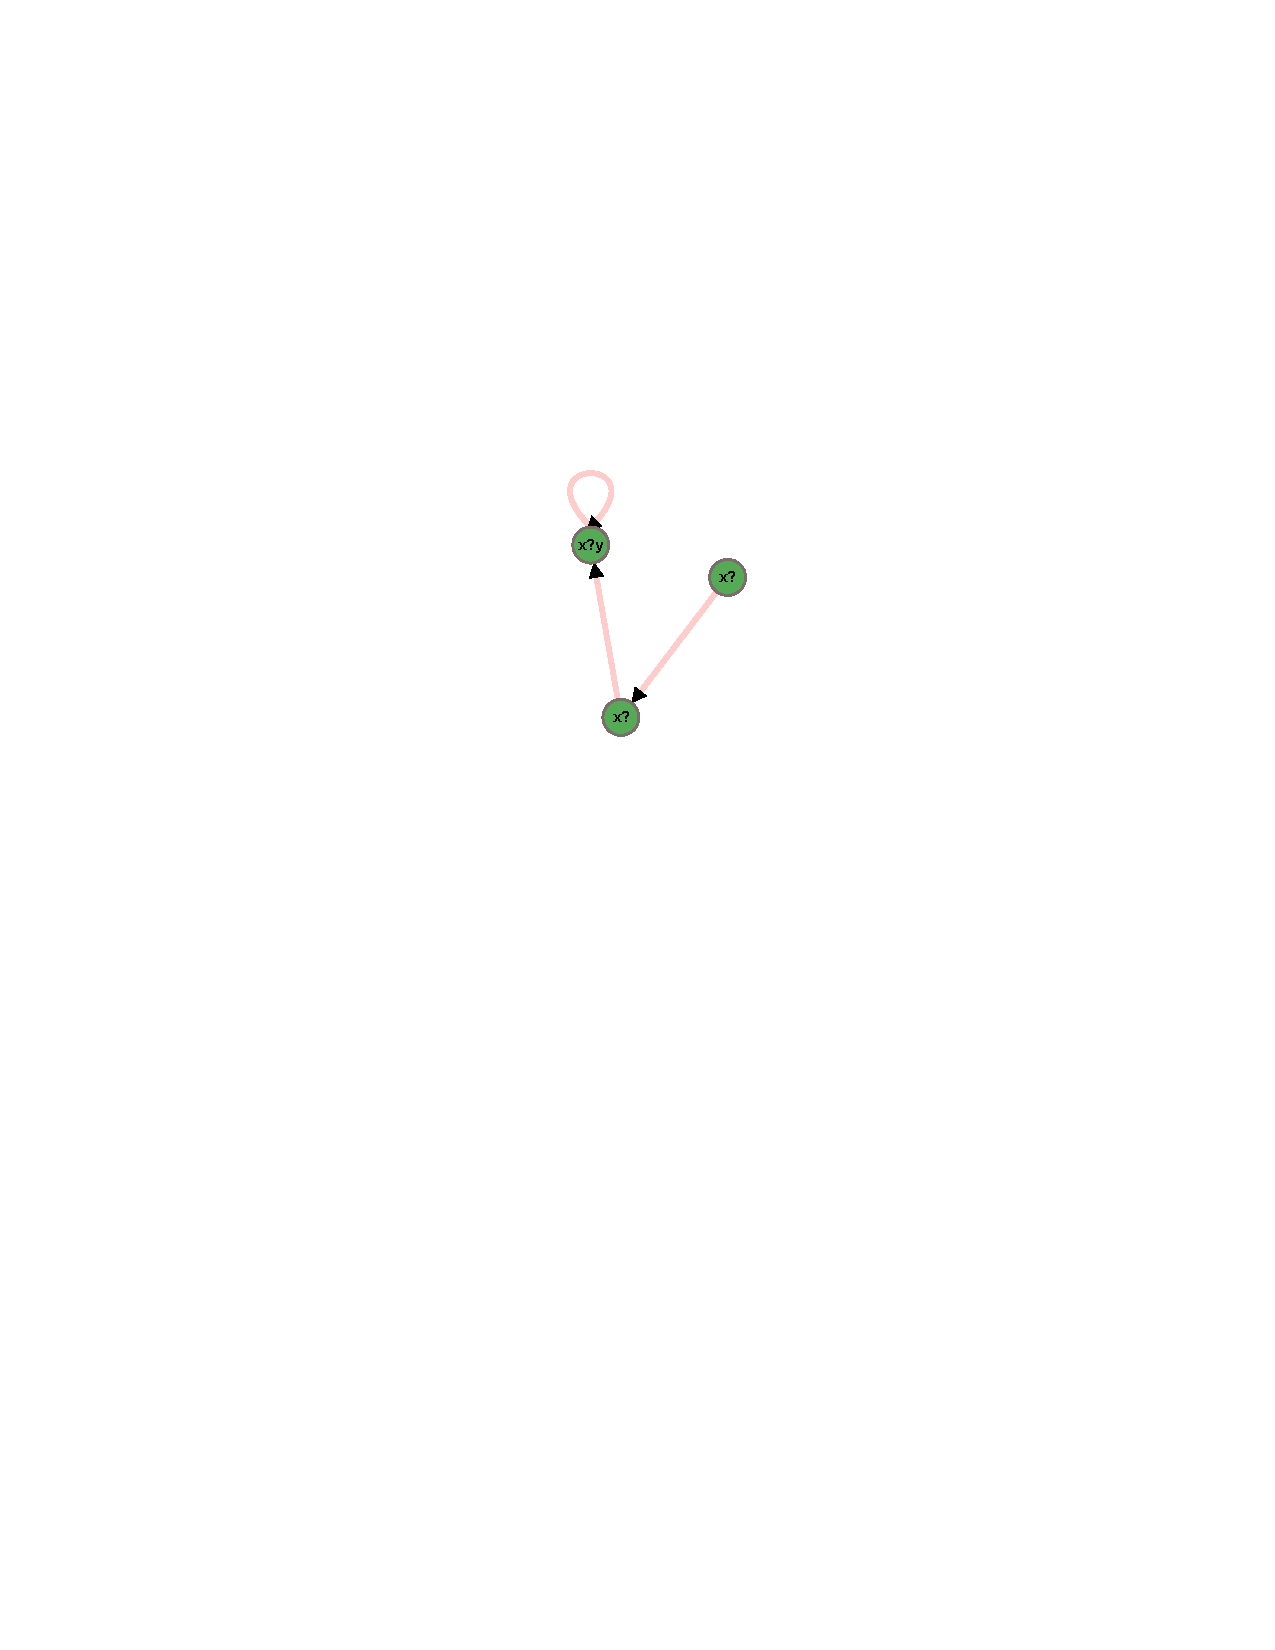
\includegraphics[width=7cm]{fig/predvar2.pdf}
  \caption{On the left, predicate $p1$ is selected, and it has values $\true$, $\false$, and $\maybe$ in order of the arrows, indicated by the appropriate colors. Then we switch the ``live'' predicate to $p2$, which happens to be $\true$ for all nodes, so the color switches to green for each node.}
  \label{fig:modifying-pred-vars}
\end{figure}

\autoref{fig:modifying-pred-vars} illustrates how predicate variable labeling looks.

\subsubsection{Modifying Edges}
Edges are represented by the map $\edgesnm: \nodesnm \times \fields \times \nodesnm \to \threevals$. For our case, since we're only dealing with a single field in the interface, the map can be simplified to $\edgesnm: \nodesnm \times \nodesnm \to \threevals$, meaning that each pair of nodes have an edge between them in either direction. For two nodes $m, n$, $\edgesnm(m, n) = \true$ implies that a green edge exists pointing from $m$ to $n$. $\edgesnm(m, n) = \maybe$ implies that the edge is light pink instead. If $\edgesnm(m, n) = \false$, then this is indicated by the absence of an edge. Once again, this is to make sure that the pattern graph isn't overly cluttered because of too many $\false$ edges. An edge is also a link for the force-directed graph in D3.

Interacting with edges is fairly simple:
\begin{itemize}
  \item Drag the mouse from a node to another to create an edge between them, in the direction of dragging.
  \item Click on an existing edge to select (or unselect) it. Selected edges appear dotted, as opposed to solid for unselected edges. Only up to one edge can be selected at a time.
  \item Press the backspace key after selecting a edge to delete it.
  \item Pressing the M key for a selected edge toggles between $\true$ and $\maybe$ values for that edge (respectively green and light pink).
  \item Pressing the R key for a selected node creates a self-loop on that node. Each node can have only one self-loop, and all edge interactions work for it just like other edges.
\end{itemize}

% Figure illustrating edge modification.
\begin{figure}
  \centering
  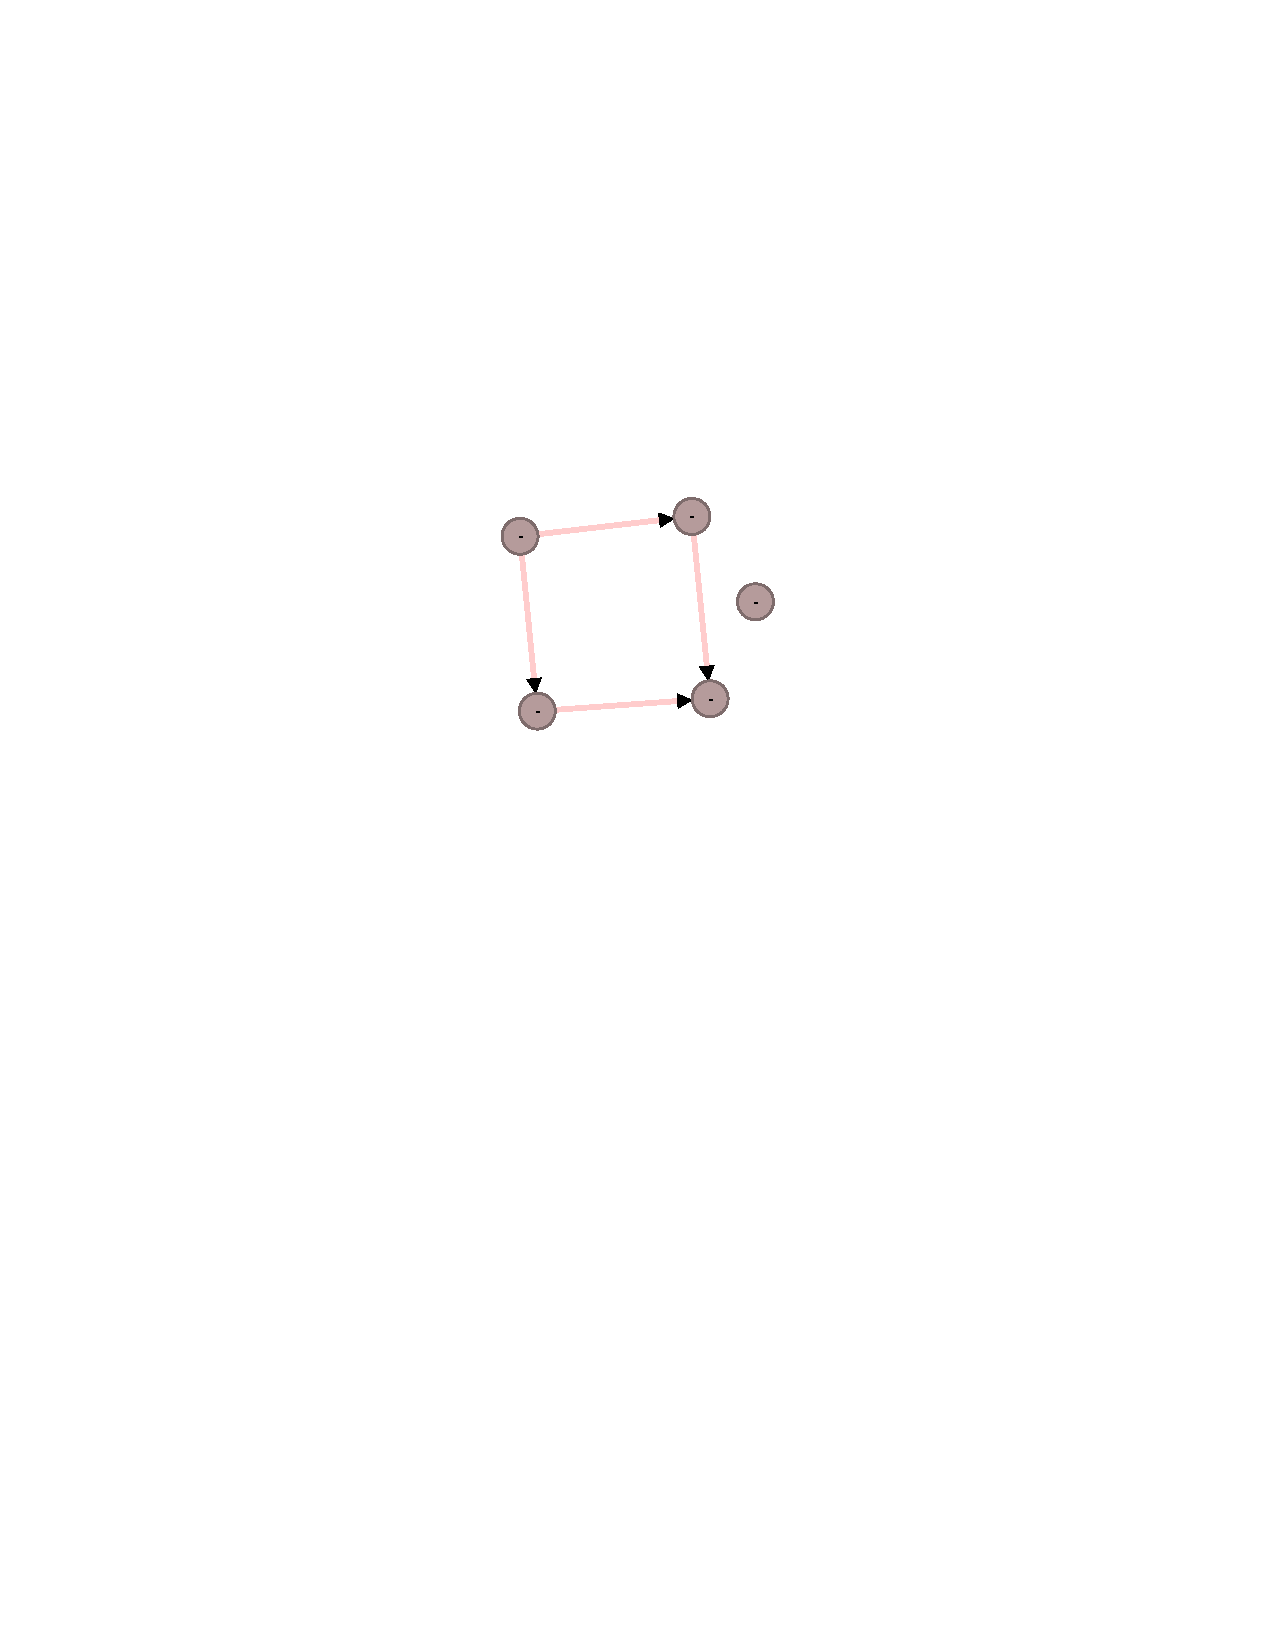
\includegraphics[width=5cm]{fig/edges1.pdf}
  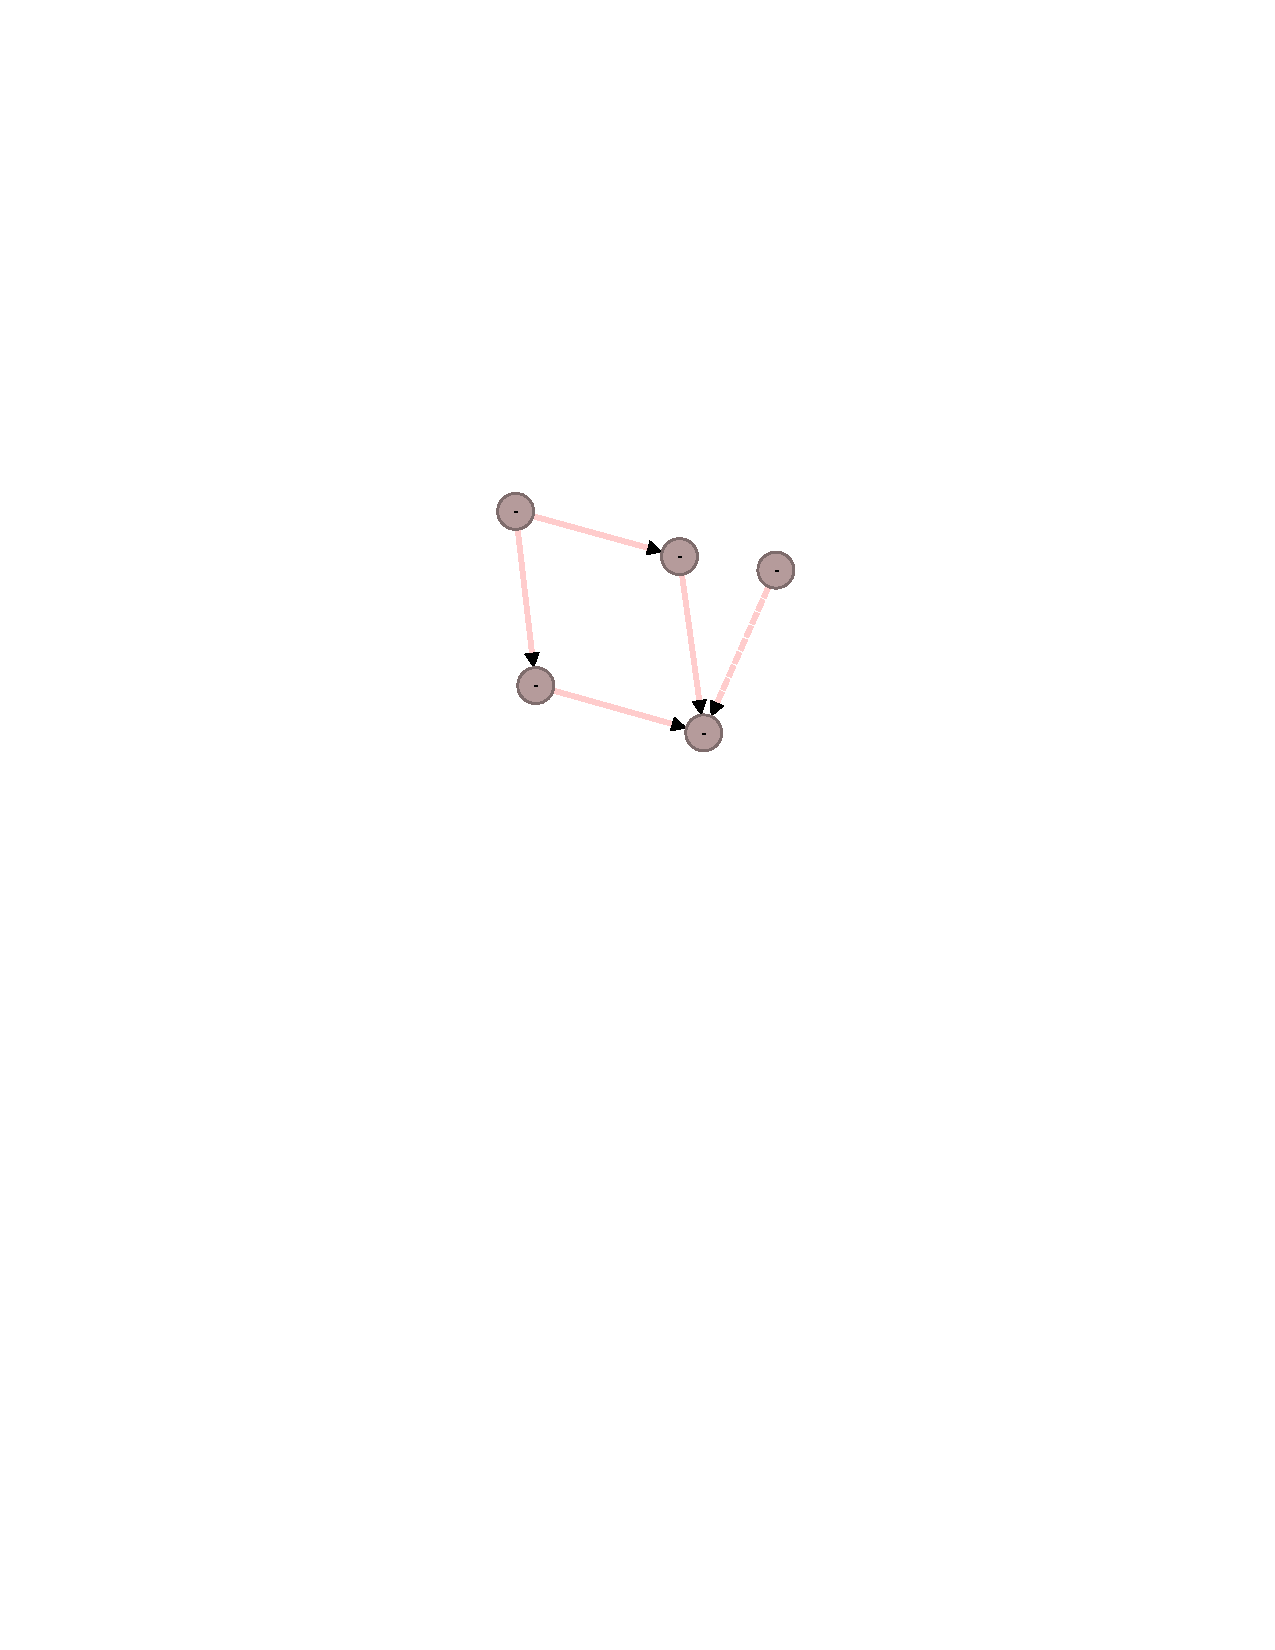
\includegraphics[width=5cm]{fig/edges2.pdf}
  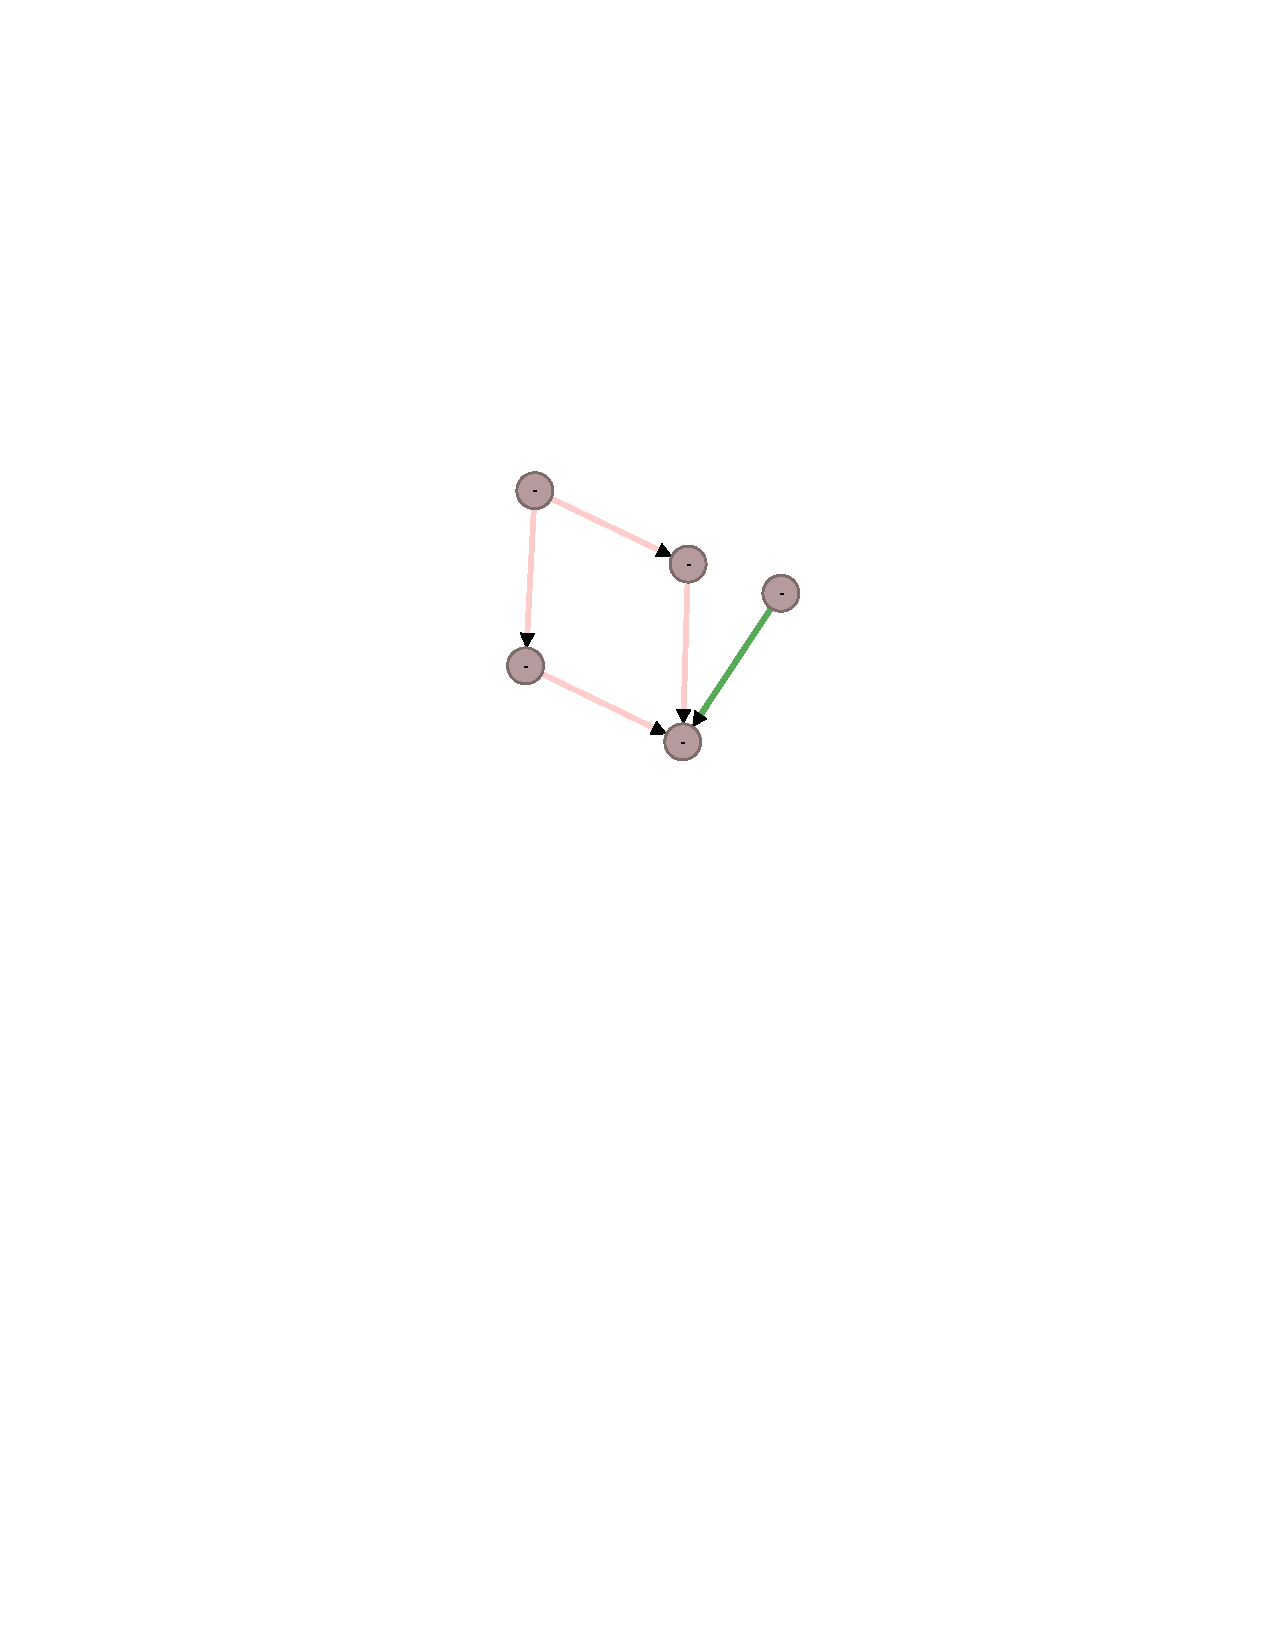
\includegraphics[width=5cm]{fig/edges3.pdf}
  \caption{The first pattern on the left has a node $n$ that is not connected to any other node. We drag from $n$ to another node to create a new edge, which is also selected in the second pattern (indicated by the dotted line). For the selected edge, we press the M key, which turns it into a $\true$ (green) edge, in the third pattern on the right.}
  \label{fig:modifying-edges}
\end{figure}

Edges are normally straight, but bidirectional edges are rounded for better visibility. \autoref{fig:modifying-edges} illustrates how the interface allows for interaction with edges.

Just like $\varlblnm$, $\edgesnm$ is not allowed to have arbitrary assignments. For instance, a $\true$ edge going out from a node implies that there cannot be any other edge going out of the same node. Our interface takes care of such constraints as follows:

\begin{itemize}
  \item Setting an edge (from node $m$ to $n$) to $\true$ sets all outgoing edges from $m$ $\false$ automatically i.e. deletes them.
  \item Setting an edge (from node $m$ to $n$) to $\maybe$ sets any $\true$ outgoing edge from $m$ to $\maybe$ automatically.
\end{itemize}

% Figure illustrating enforcement of edge constraints.
\begin{figure}
  \centering
  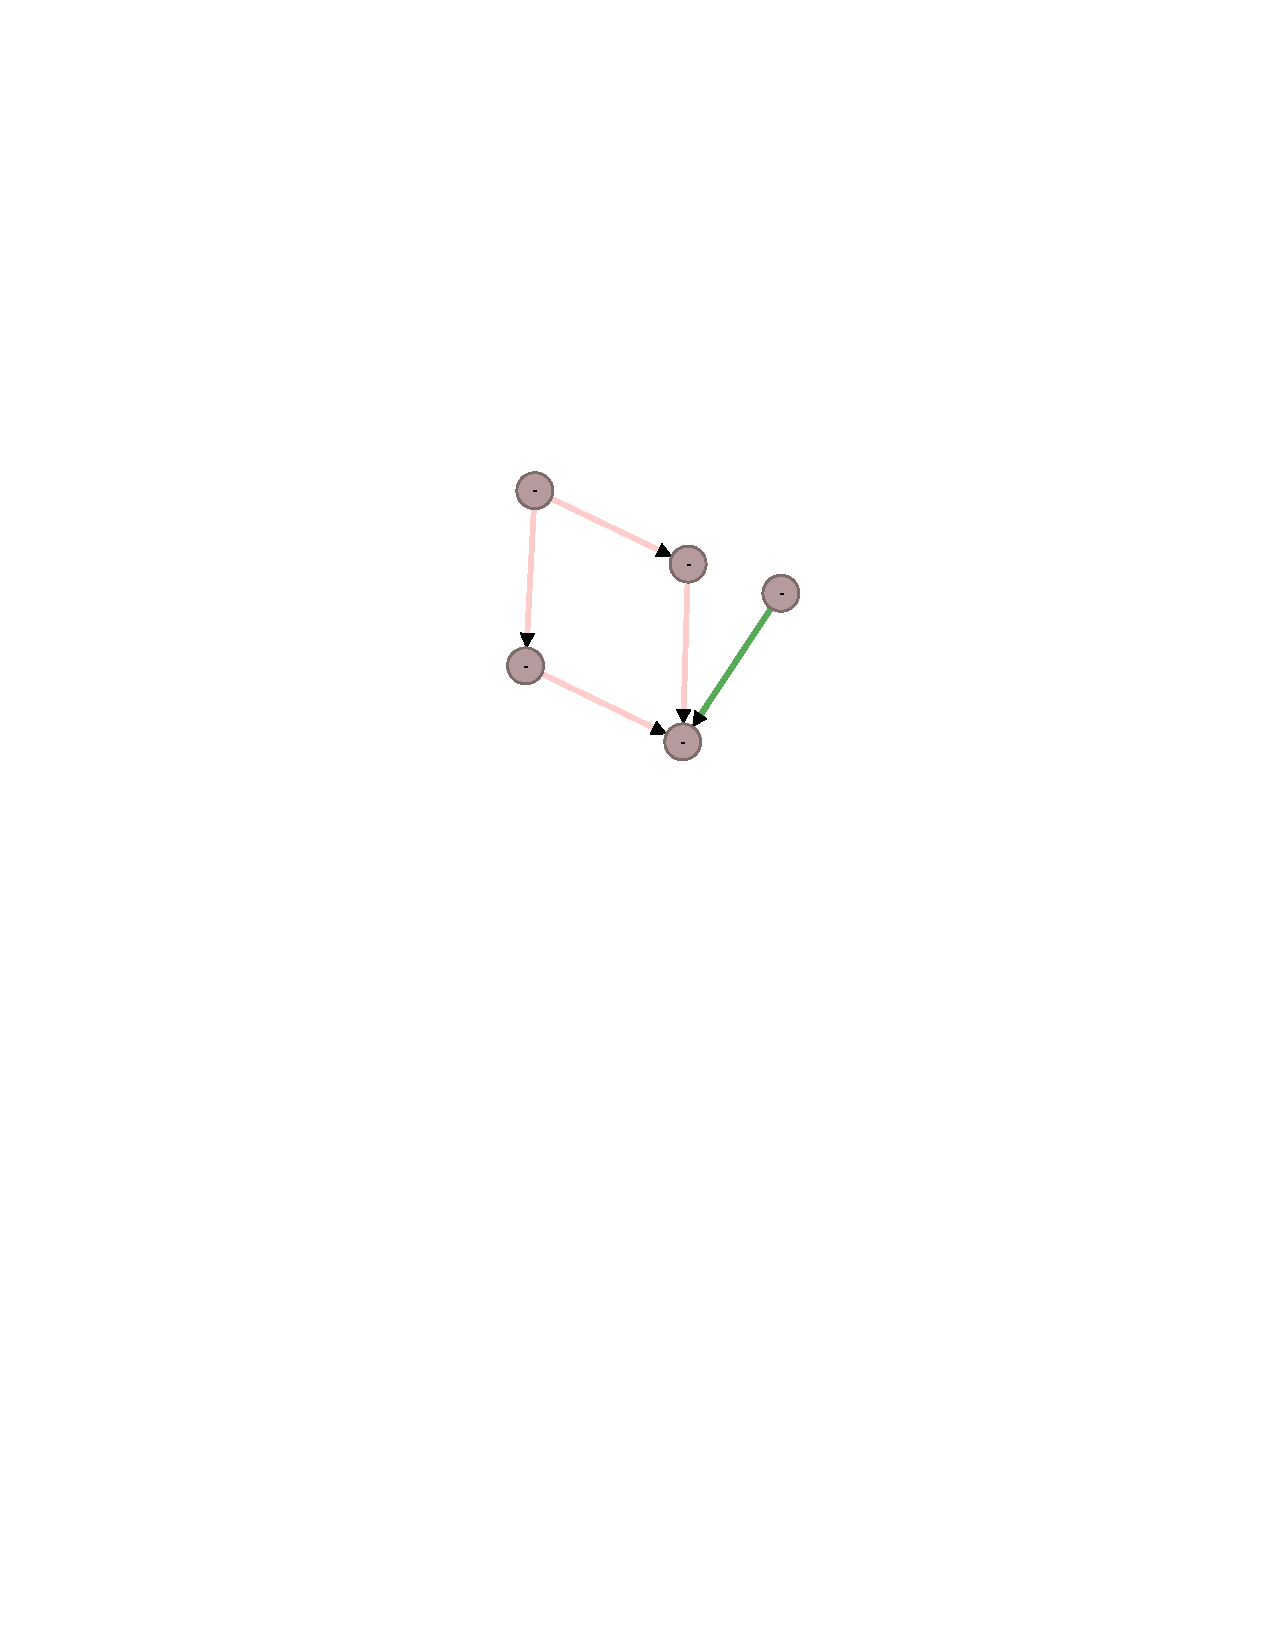
\includegraphics[width=5cm]{fig/edges3.pdf}
  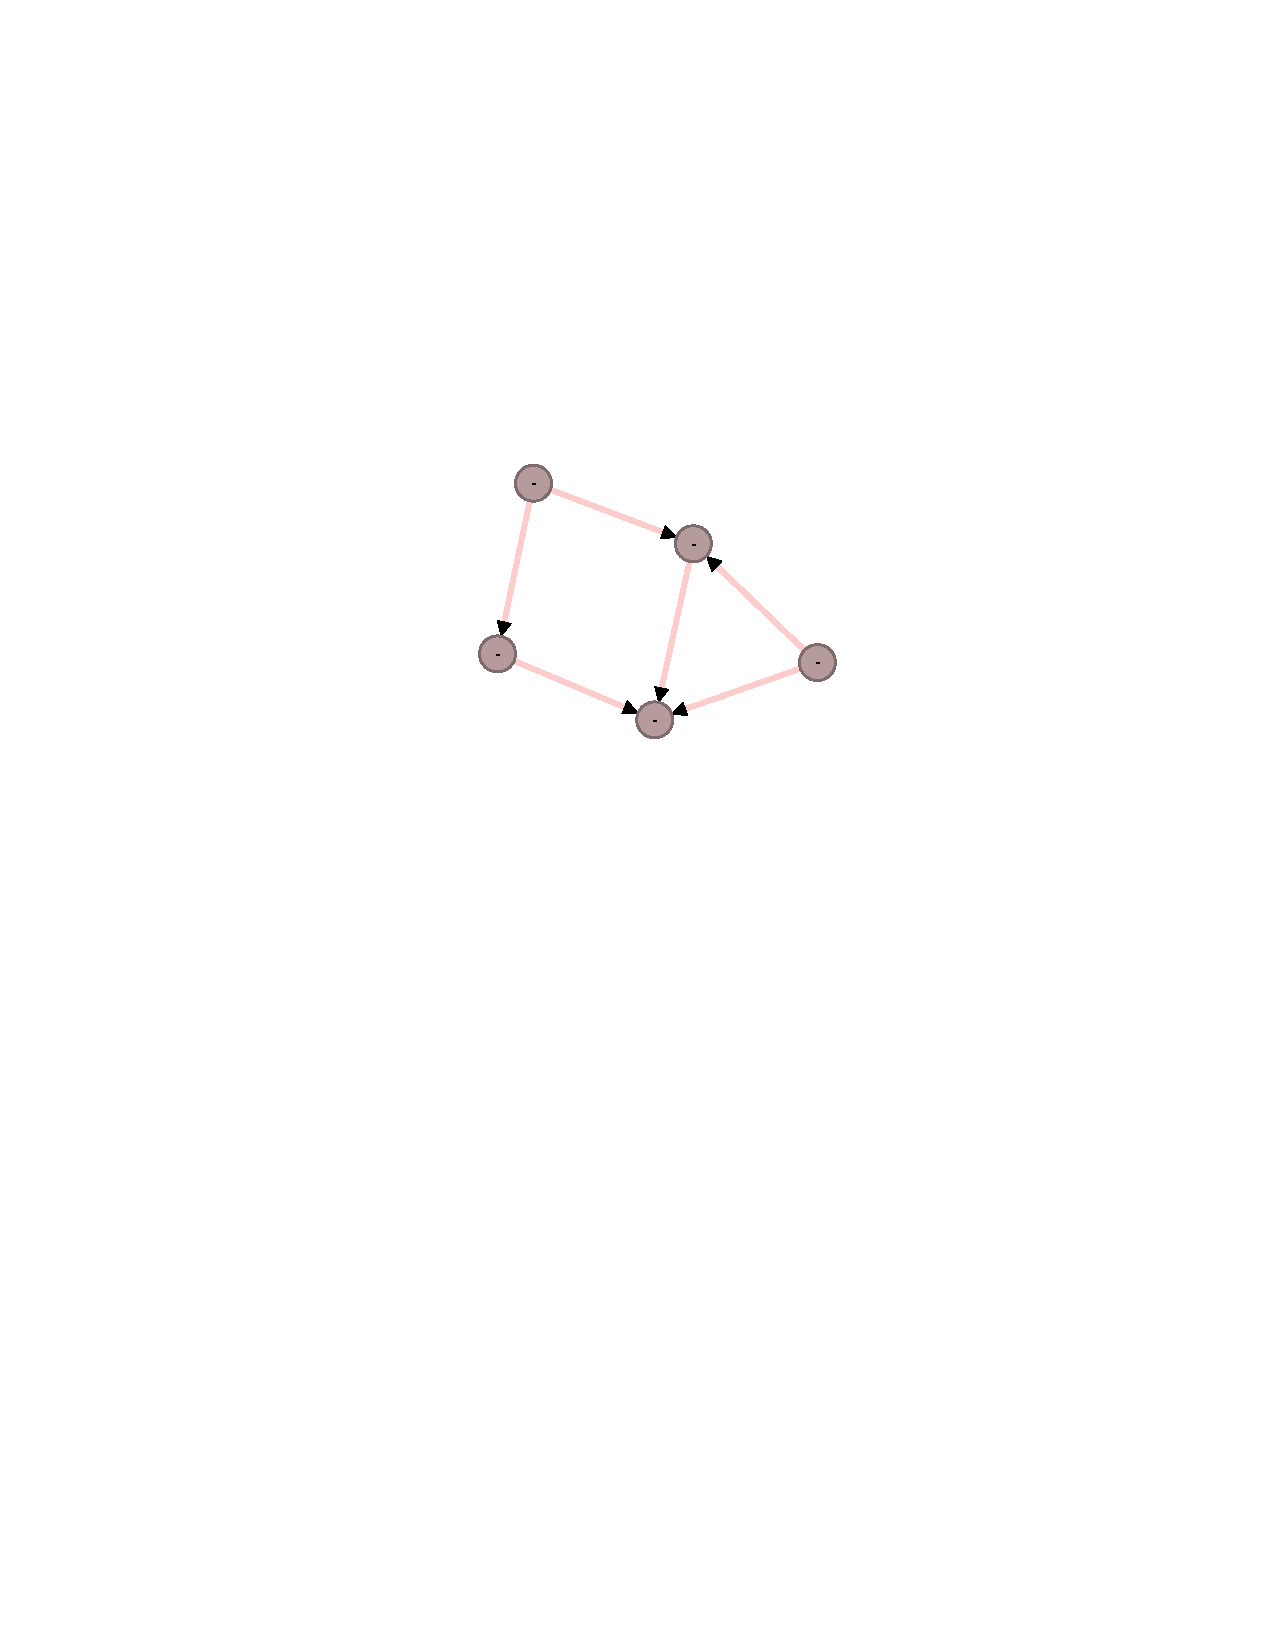
\includegraphics[width=5cm]{fig/edge-constraints-1.pdf}
  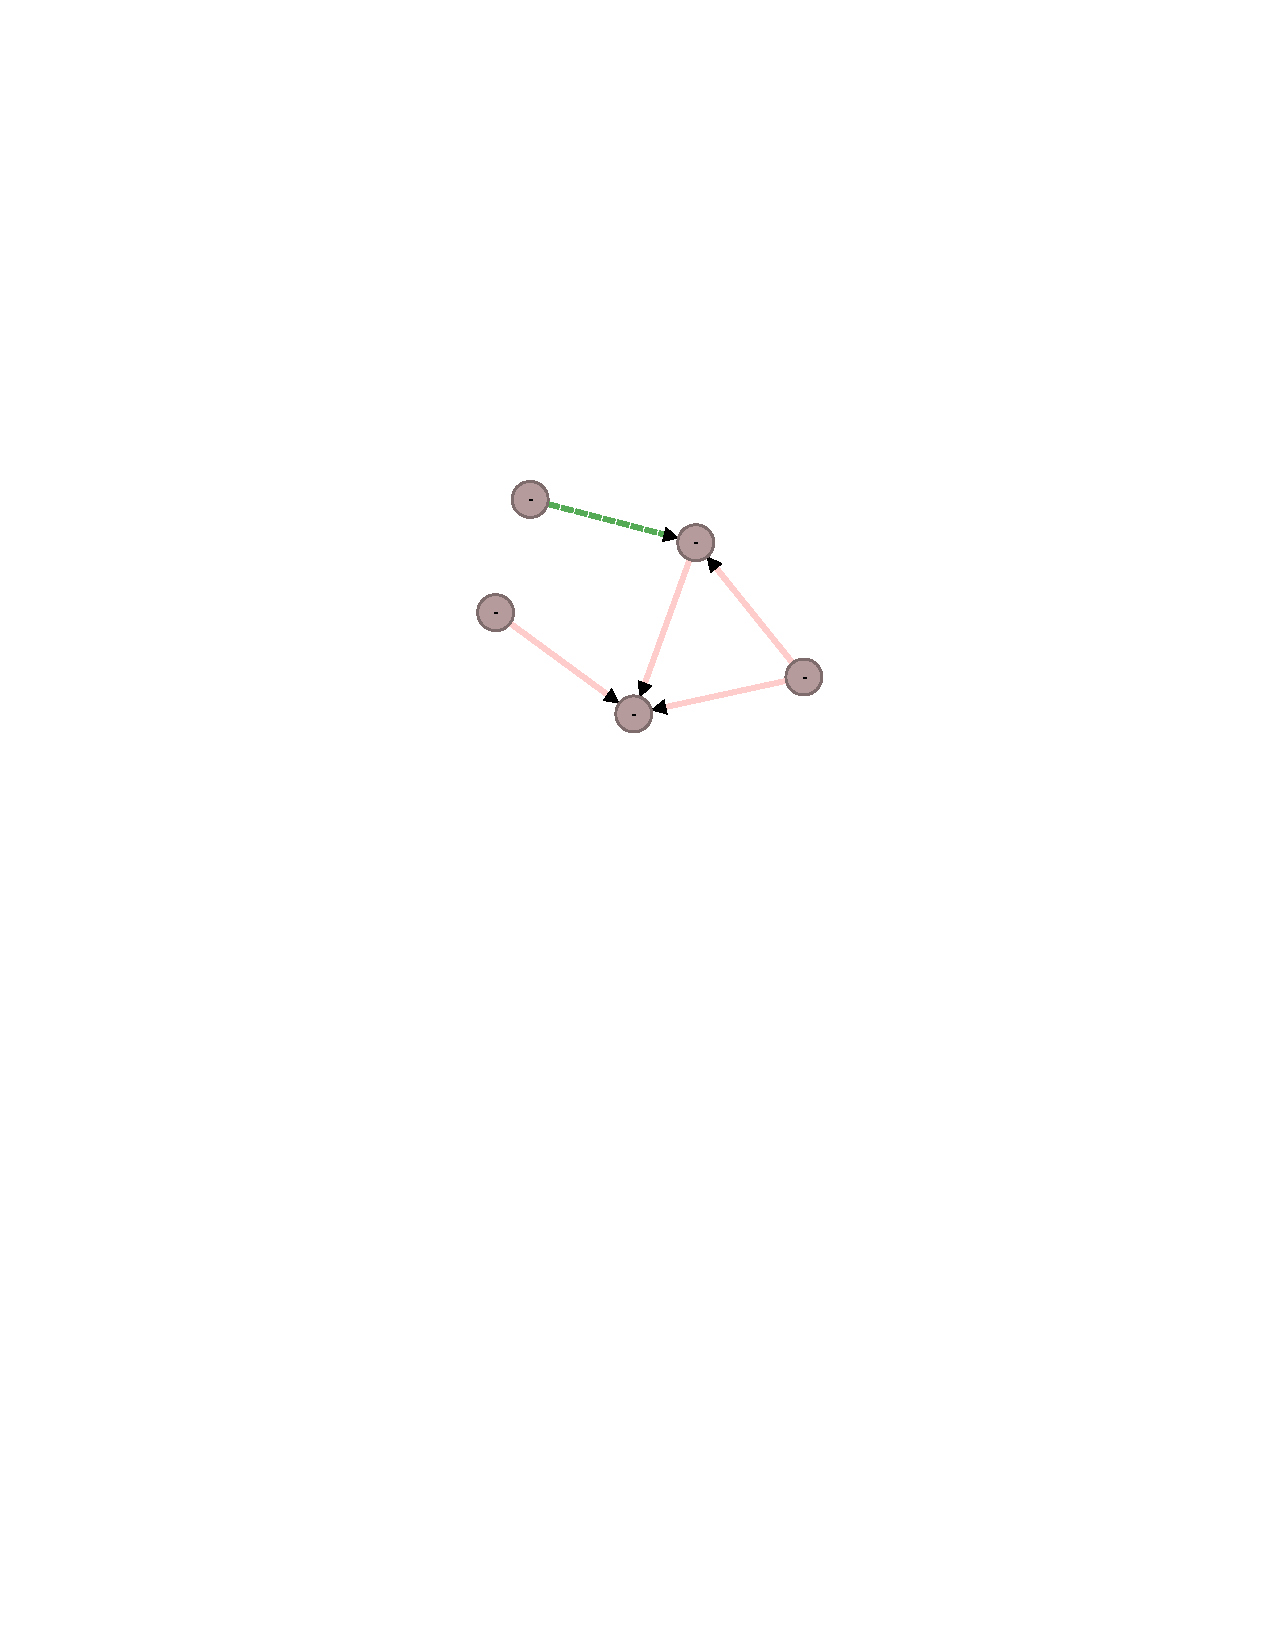
\includegraphics[width=5cm]{fig/edge-constraints-2.pdf}
  \caption{The first figure on the left has a node $n$ with a $\true$ outgoing edge. We create another outgoing edge from $n$, which is a $\maybe$ edge by default, but it also turns the $\true$ edge to $\maybe$. In the third pattern on the right, we turn a $\maybe$ edge to $\true$, which results in the other $\maybe$ edge going out of it disappearing (becoming $\false$).}
  \label{fig:edge-constraints}
\end{figure}

\autoref{fig:edge-constraints} illustrates how constraints on $\edgesnm$ are enforced by the interface.

\subsubsection{Modifying the Summary Function}
The summary function $\sigma: \nodesnm \to \bools$ indicates where a node is a summary node. Our interface indicates summary nodes by making them larger than other nodes. Selecting a node and pressing the S key toggles the value of $\sigma$ for that node. \autoref{fig:summary-nodes} illustrates an example of this.

% Figure illustrating pred var modification.
\begin{figure}
  \centering
  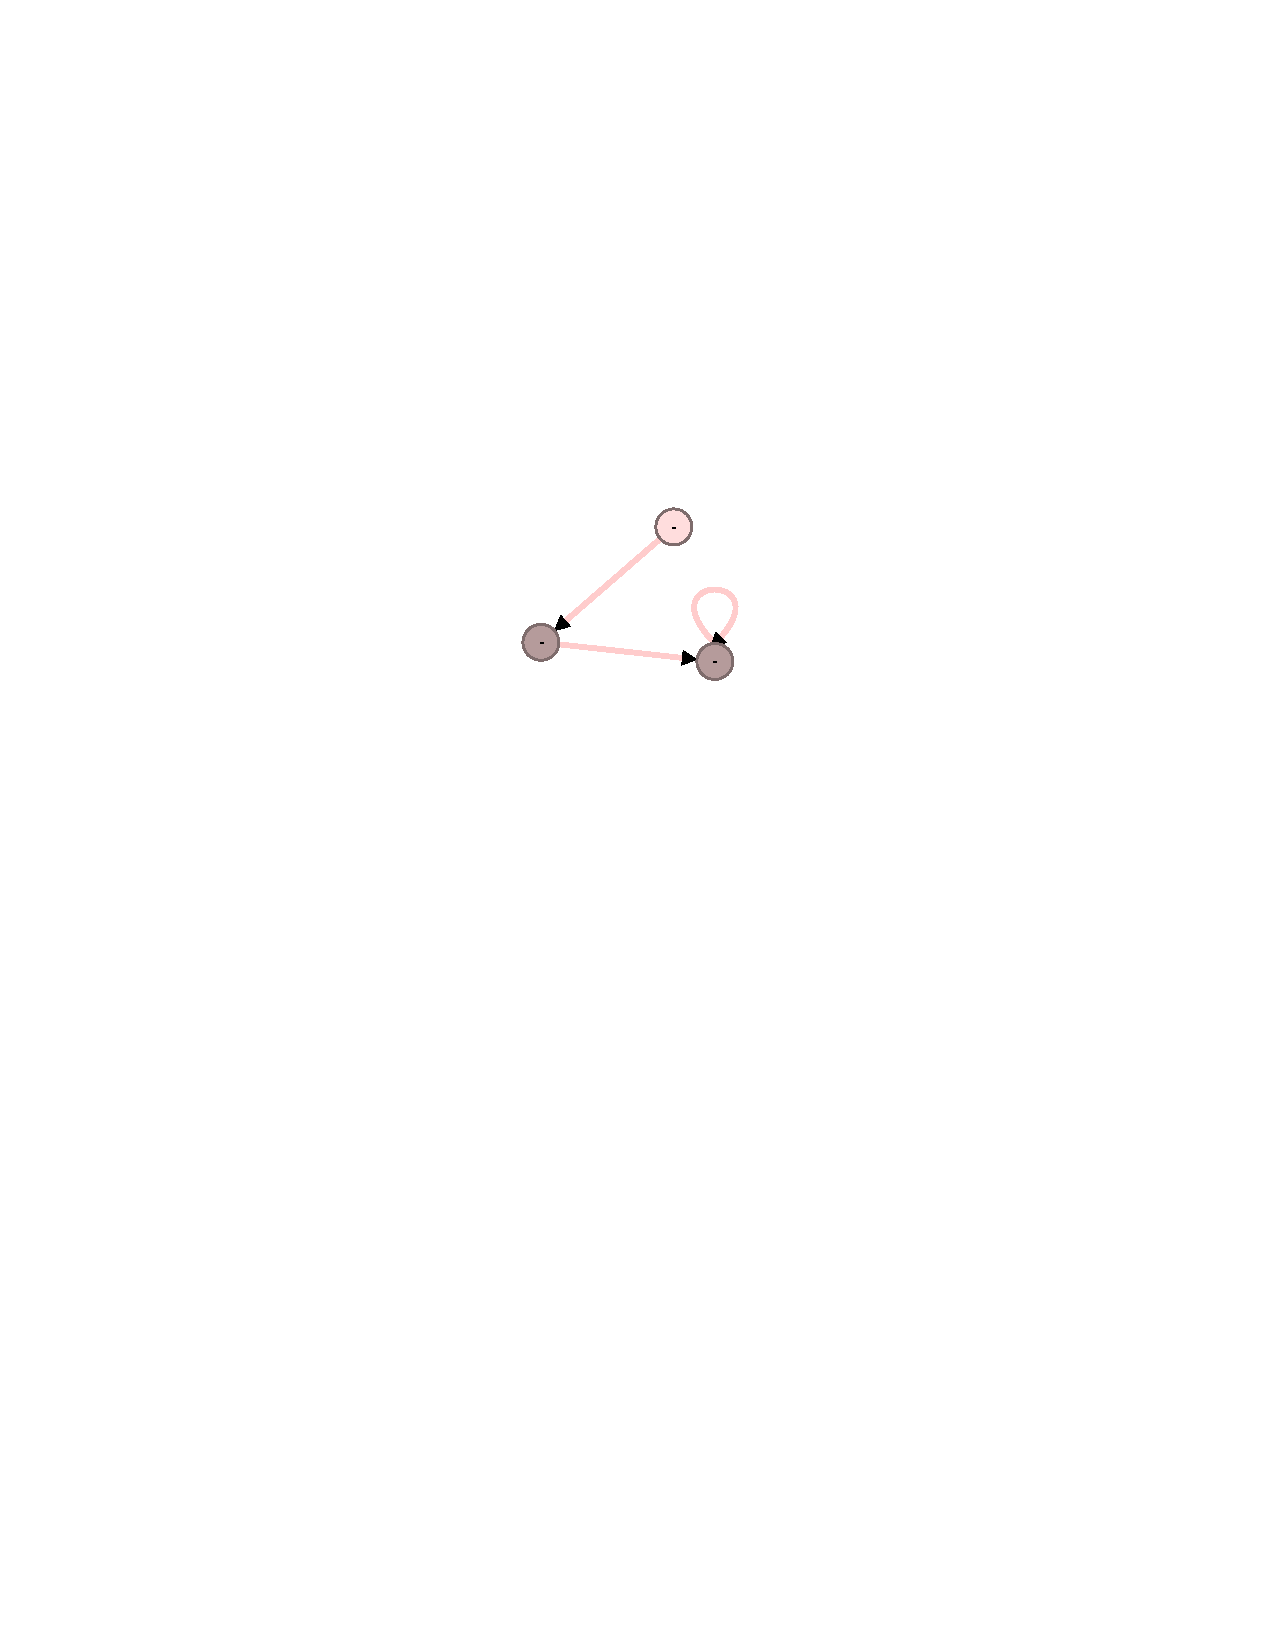
\includegraphics[width=7cm]{fig/summary1.pdf}
  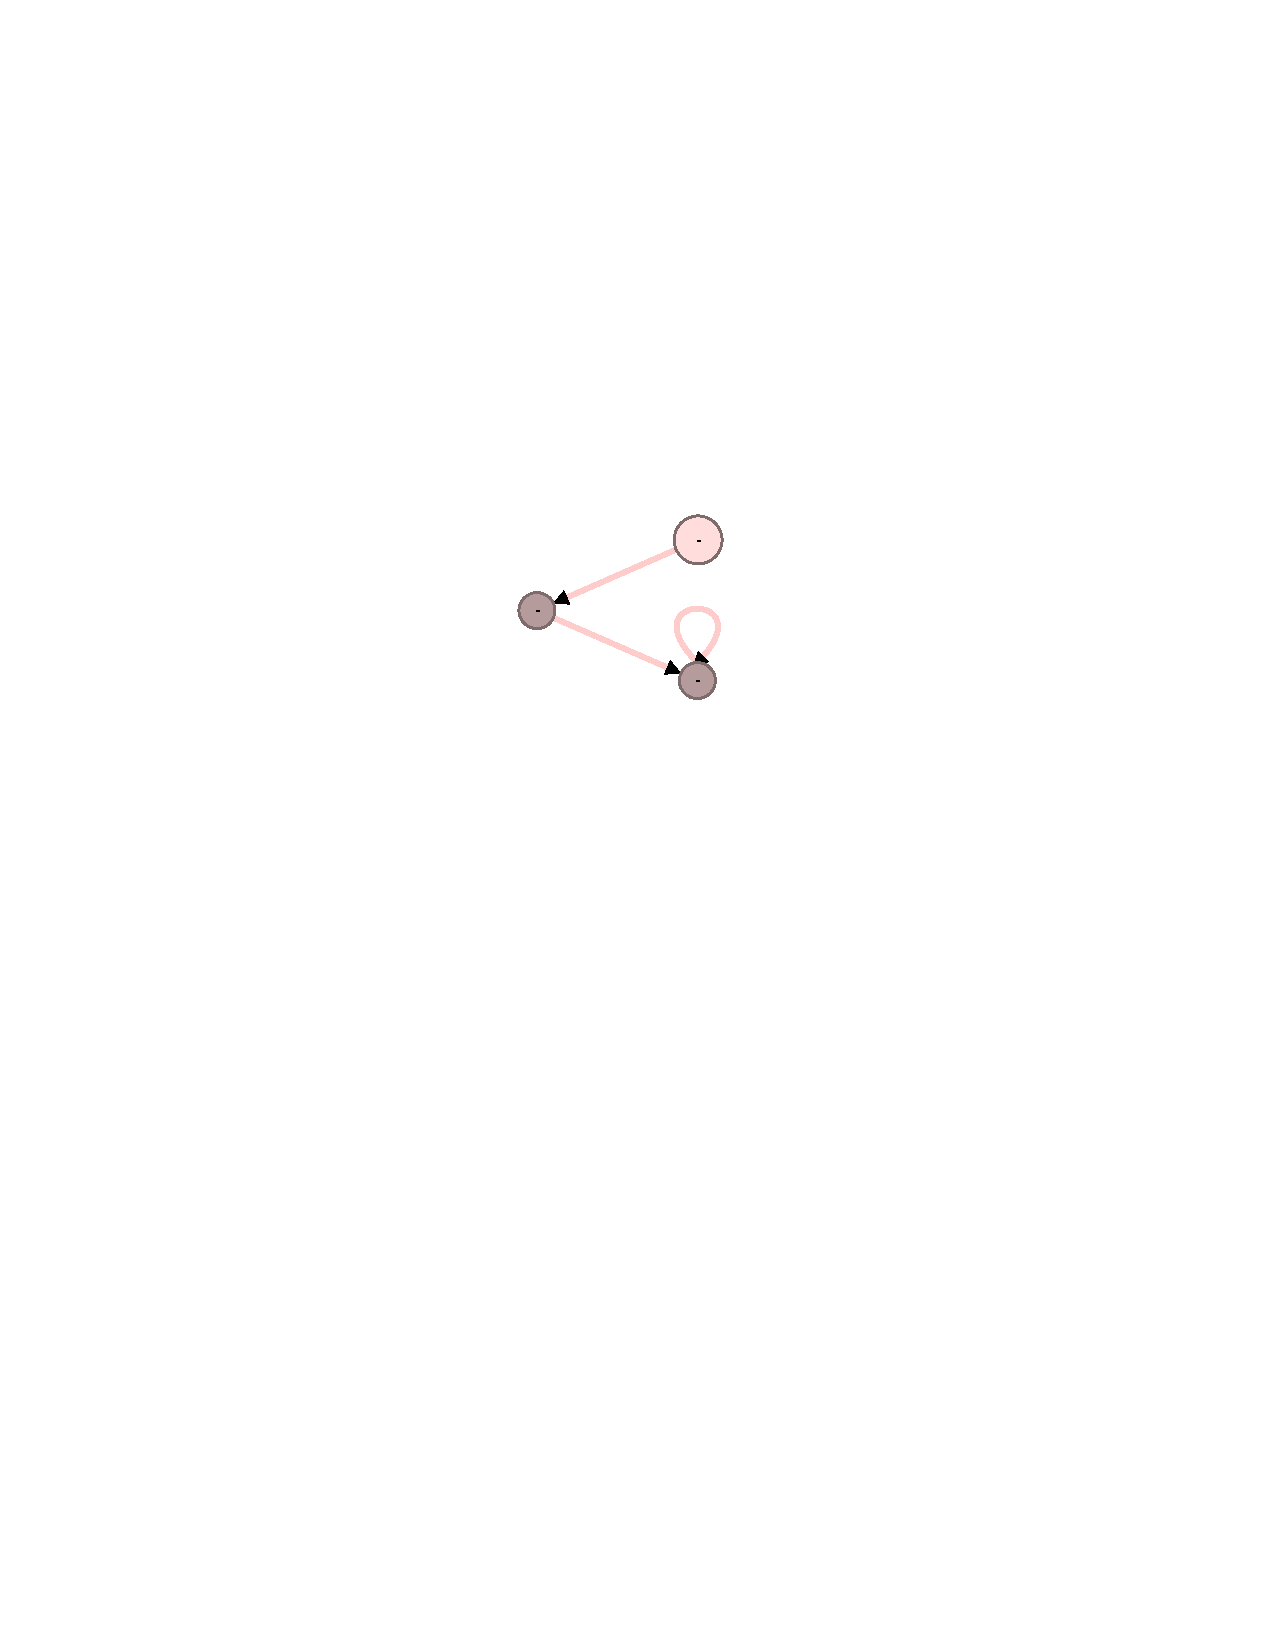
\includegraphics[width=7cm]{fig/summary2.pdf}
  \caption{The pattern on the left has three nodes, one of which is selected. On pressing the S key, it becomes a summary node, indicated by the larger size in the pattern on the right.}
  \label{fig:summary-nodes}
\end{figure}

\section{User Interaction}
The generated patterns are used by the \verifier algorithm as candidates for annotating vertices in the program unwinding tree. The following steps describe how interaction with the user works. We will later elaborate the same with an example.

\begin{enumerate}
  \item At any point, interaction with the Oracle (human user) is limited to requested patterns for a single vertex of the program unwinding tree.
  \item Start with $H^{+} = H^{-} = \{\}$. At this point, the user can provide an arbitrary pattern to begin with.
  \item If the pattern (we call it $C$) is such that $\forall h \in H^{+}, h \matchedby C$ and $\forall h \in H^{-}, h \not \matchedby C$, then C is sent to the verifier. On the other hand, if there is any heap in the existing sets $H^{+}, H^{-}$ for which these conditions are not satisfied, it is highlighted to the user.
  \item If the pattern is accepted in \autoref{alg:newcandidate}, then no more input is requested from the user.
  \item If the pattern is not accepted, one or both of $H^{+}$ or $H^{-}$ are updated, and the user needs to update the provided pattern. Return to Step 3.
\end{enumerate}

As described in \autoref{defn:heap-pat}, each individual heap can also be presented as a pattern that represents exactly that heap. As a result, all the individual heaps in $H^{+}$ and $H^{-}$ are also patterns, but with limited properties and and no $\maybe$ assignments to variables and edges, and no summary nodes. We now present an example to illustrate how the above steps work.

\subsection{Illustrating User Interaction}
\label{sec:illustrating-user-interaction}
We note that all heaps have a special \nilconst node, which represents the \nullconst address. \nilconst nodes cannot be summary nodes, and have no outgoing edges. In this example, we consider the program \altlistsimplified in \autoref{fig:alt-list-simplified} that creates a linked list with alternating $\true$ and $\false$ values for the predicate $p$.

\begin{figure}
  \centering
  \begin{Verbatim}[commandchars=\\\{\},codes={\catcode`\$=3\catcode`\^=7\catcode`\_=8}]
\PY{k+kt}{void} \PY{n+nf}{alt\PYZus{}list}\PY{p}{(}\PY{p}{)} \PY{p}{\PYZob{}}
  \PY{k+kt}{bool} \PY{n}{d} \PY{o}{=} \PY{n}{TRUE}\PY{p}{;}
  \PY{n}{List} \PY{n}{l} \PY{o}{=} \PY{n}{cons}\PY{p}{(}\PY{n}{d}\PY{p}{,} \PY{n}{NIL}\PY{p}{)}\PY{p}{;}
  \PY{c+c1}{// LOOP\PYZhy{}CONS: build a list with alternating Boolean values.}
  \PY{k}{while} \PY{p}{(}\PY{n}{non\PYZus{}det}\PY{p}{(}\PY{p}{)}\PY{p}{)} \PY{p}{\PYZob{}}
    \PY{n}{d} \PY{o}{=} \PY{o}{!}\PY{n}{d}\PY{p}{;}
    \PY{n}{l} \PY{o}{=} \PY{n}{cons}\PY{p}{(}\PY{n}{d}\PY{p}{,} \PY{n}{l}\PY{p}{)}\PY{p}{;}
  \PY{p}{\PYZcb{}}
  \PY{c+c1}{// LOOP\PYZhy{}CHK: check that the Boolean values alternate.}
  \PY{k}{while} \PY{p}{(}\PY{n}{l} \PY{o}{!}\PY{o}{=} \PY{n}{NIL}\PY{p}{)} \PY{p}{\PYZob{}}
    \PY{n}{assert}\PY{p}{(}\PY{n}{l}\PY{o}{\PYZhy{}}\PY{o}{\PYZgt{}}\PY{n}{data} \PY{o}{=}\PY{o}{=} \PY{n}{d}\PY{p}{)}\PY{p}{;}
    \PY{n}{d} \PY{o}{=} \PY{o}{!}\PY{n}{d}\PY{p}{;}
    \PY{n}{l} \PY{o}{=} \PY{n}{l}\PY{o}{\PYZhy{}}\PY{o}{\PYZgt{}}\PY{n}{next}\PY{p}{;}
  \PY{p}{\PYZcb{}}
  \PY{k}{return}\PY{p}{;}
\PY{p}{\PYZcb{}}
\end{Verbatim}

  \caption{\altlistsimplified: a slightly modified and simplified version of the SV-COMP benchmark program \altlist (\autoref{fig:alt-list}) that constructs a list with cells that store alternating Boolean values for a known predicate. We will demonstrate concrete heaps and patterns for the prgram location at the label \checkpoint.}
  \label{fig:alt-list-simplified}
\end{figure}

The user is not expected to know what the program or the verification algorithm does, and will only be presented with examples. User insight is expected based solely on those. We assume that only a single predicate $p \in \predvars$ exists, so all node colors only refer to that single predicate. We start with $H^{+} = H^{-} = \{\}$, at which point the user can't really provide any insight. It might be worthwhile to have a default candidate be provided by the interface itself at this point, but we still leave it to the user just in case they have additional insight about the program from other sources. Suppose the user just provides a pattern with a single node labeled \nilconst (\autoref{fig:nil-node}).

% Just the nil node.
\begin{figure}
  \centering
  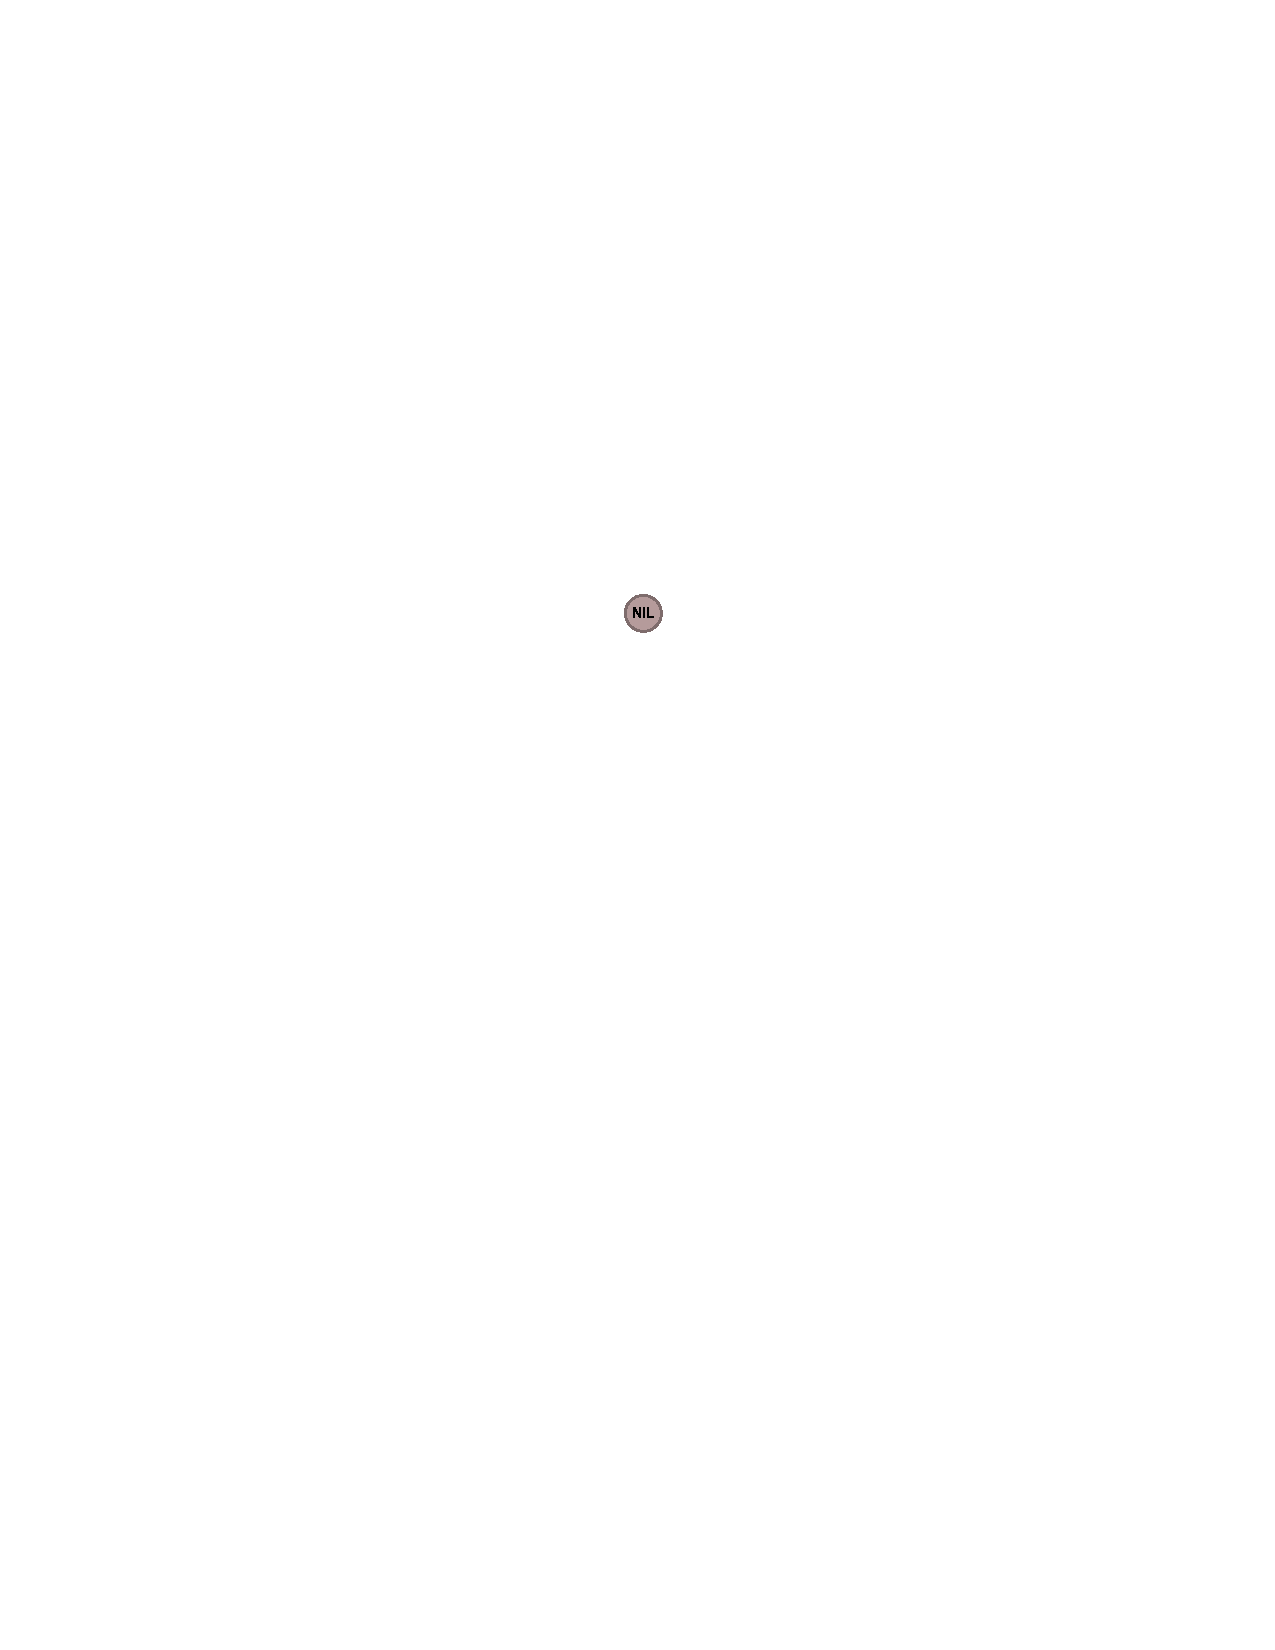
\includegraphics[width=5cm]{fig/just-nil.pdf}
  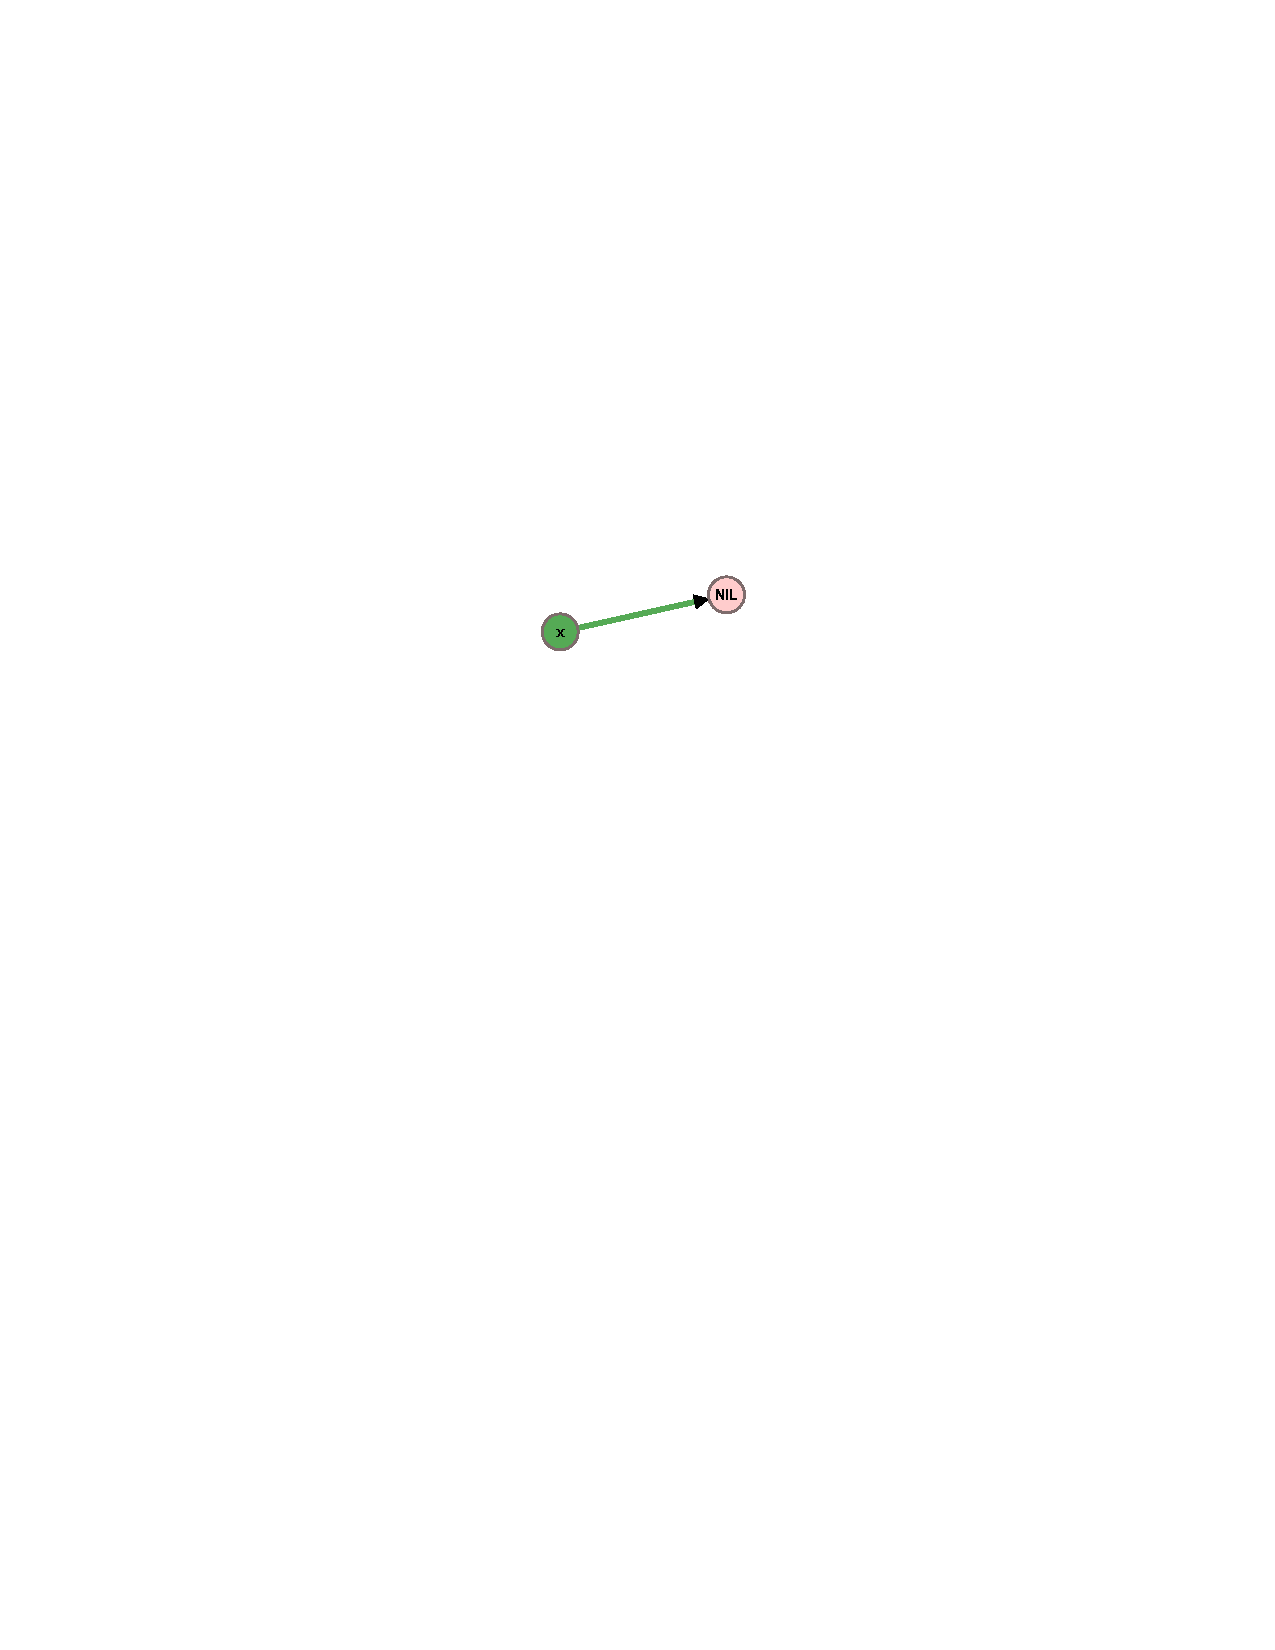
\includegraphics[width=5cm]{fig/positive1.pdf}
  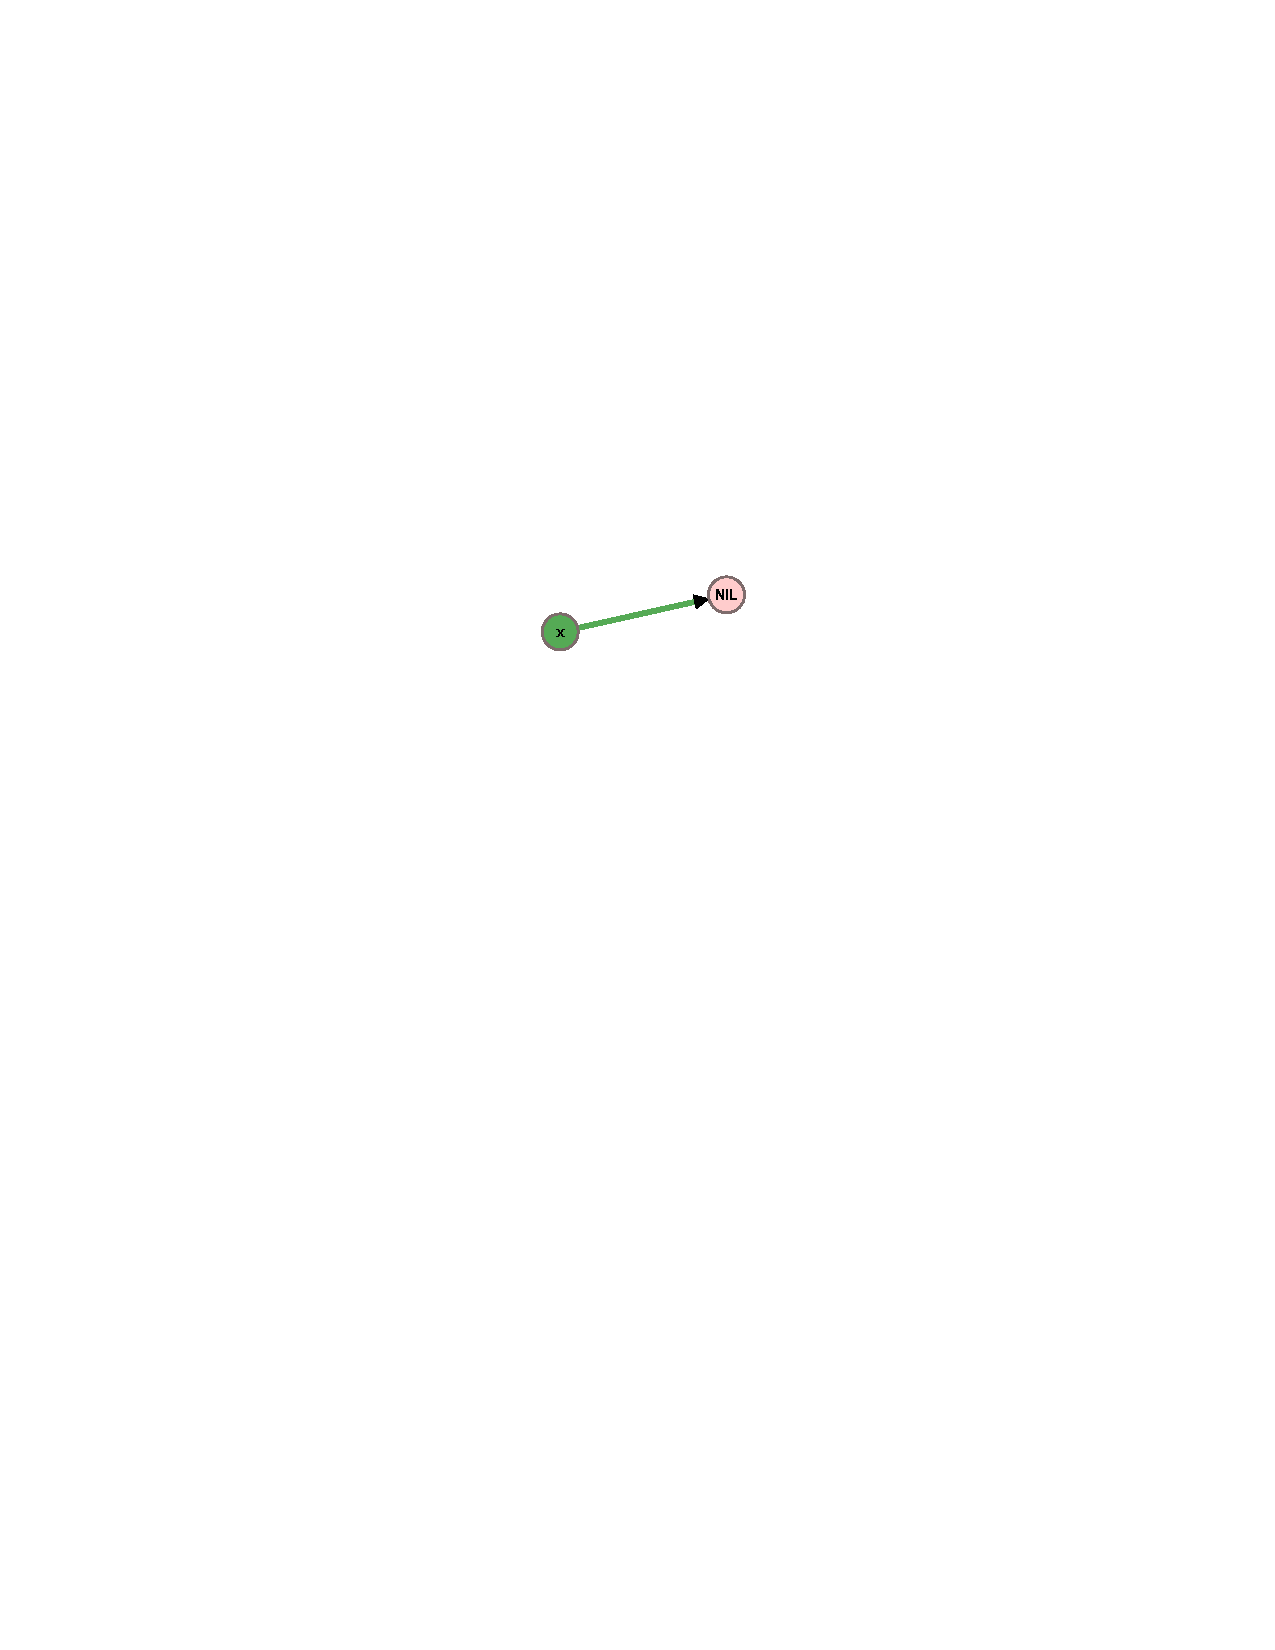
\includegraphics[width=5cm]{fig/positive1.pdf}
  \caption{On the left is the initial pattern candidate provided by the user. At this point, the user does not know what the program is doing, or what program location the candidate is being requested for. As a response, the verifier returns the concrete heap in the center as a positive example, indicating that the pattern provided by the user should be able to cover it. The user in response eagerly provides the same positive example as a candidate pattern.}
  \label{fig:nil-node}
\end{figure}

At this point, we get a new concrete heap back from the verifier (\autoref{fig:nil-node}). The user once again tries to respond in a simple way by providing the heap returned by the verifier as a pattern (\autoref{fig:nil-node}). In response to the pattern provided by the user, the verifier returns a new heap as part of $H^{+}$, shown in \autoref{fig:positive-examples}.

% Some positive examples.
\begin{figure}
  \centering
  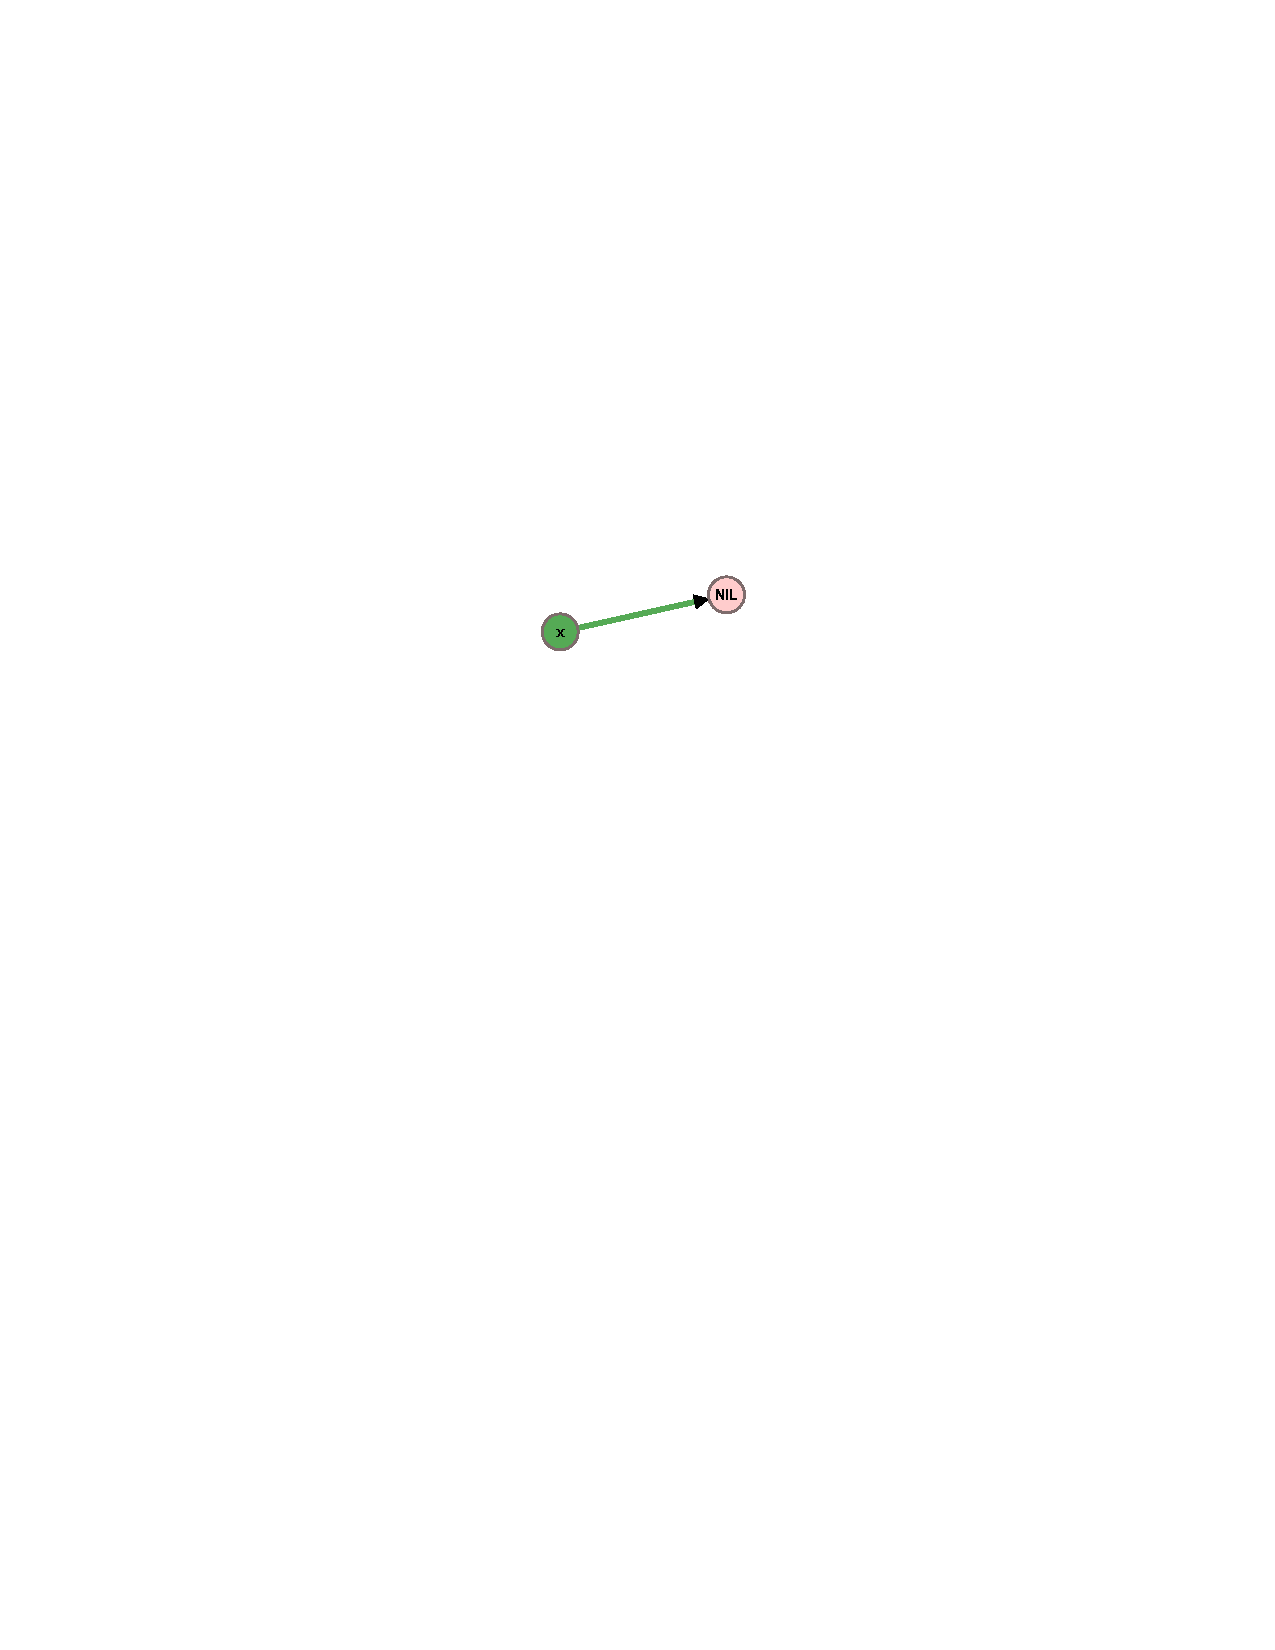
\includegraphics[width=7cm]{fig/positive1.pdf}
  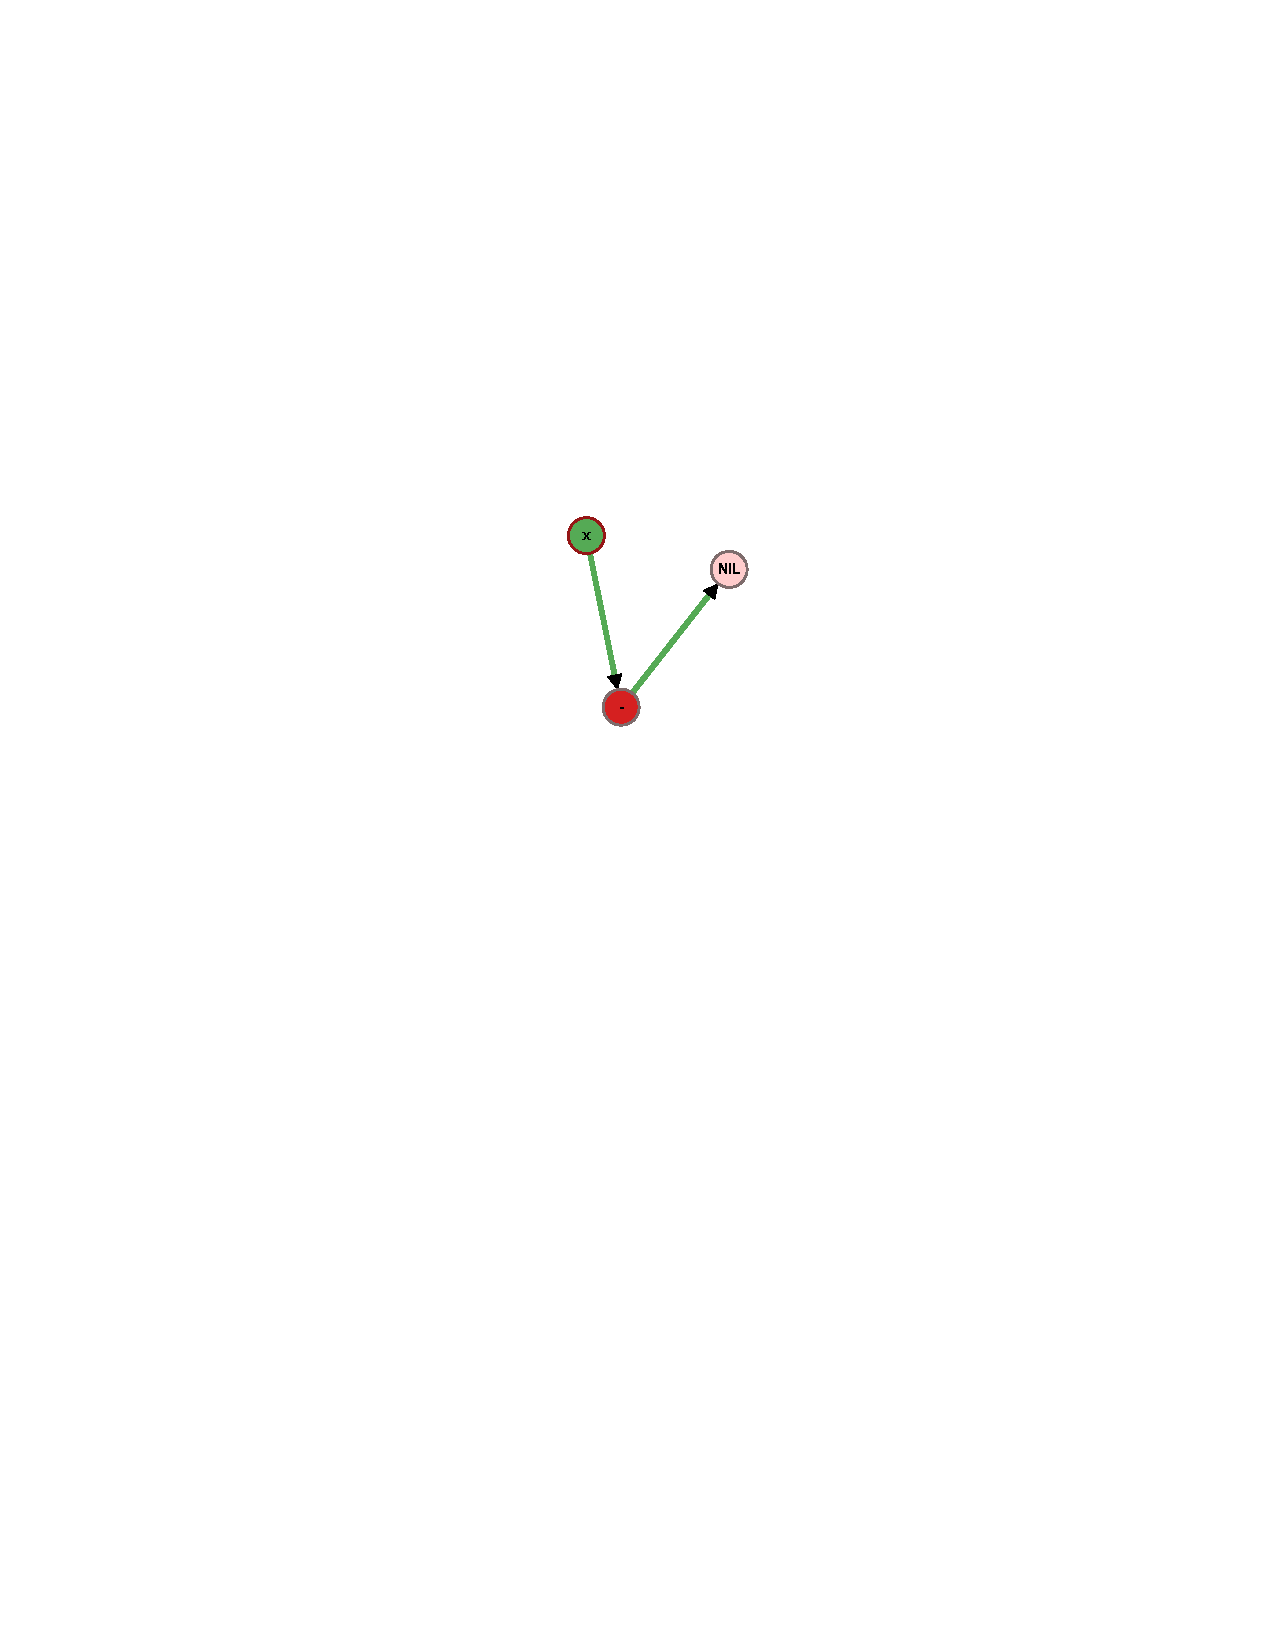
\includegraphics[width=7cm]{fig/positive2.pdf}
  \caption{The set $H^{+}$ after the user has provided two candidate patterns to the verifier.}
  \label{fig:positive-examples}
\end{figure}

Now is the first time the user needs to think of a non-trivial pattern, because the two heaps we have in $H^{+}$ are very different. At this point, the user makes two attempts, a wrong one and a right one, and we describe what happens in each case in \autoref{fig:pattern-attempts}. The right pattern uses a summary node, because summary nodes can abstract out zero or more concrete nodes. Similarly, $\maybe$ edges are used to indicate that the edge may or may not actually exist in a concrete pattern represented by the heap pattern.

% Some candidates.
\begin{figure}
  \centering
  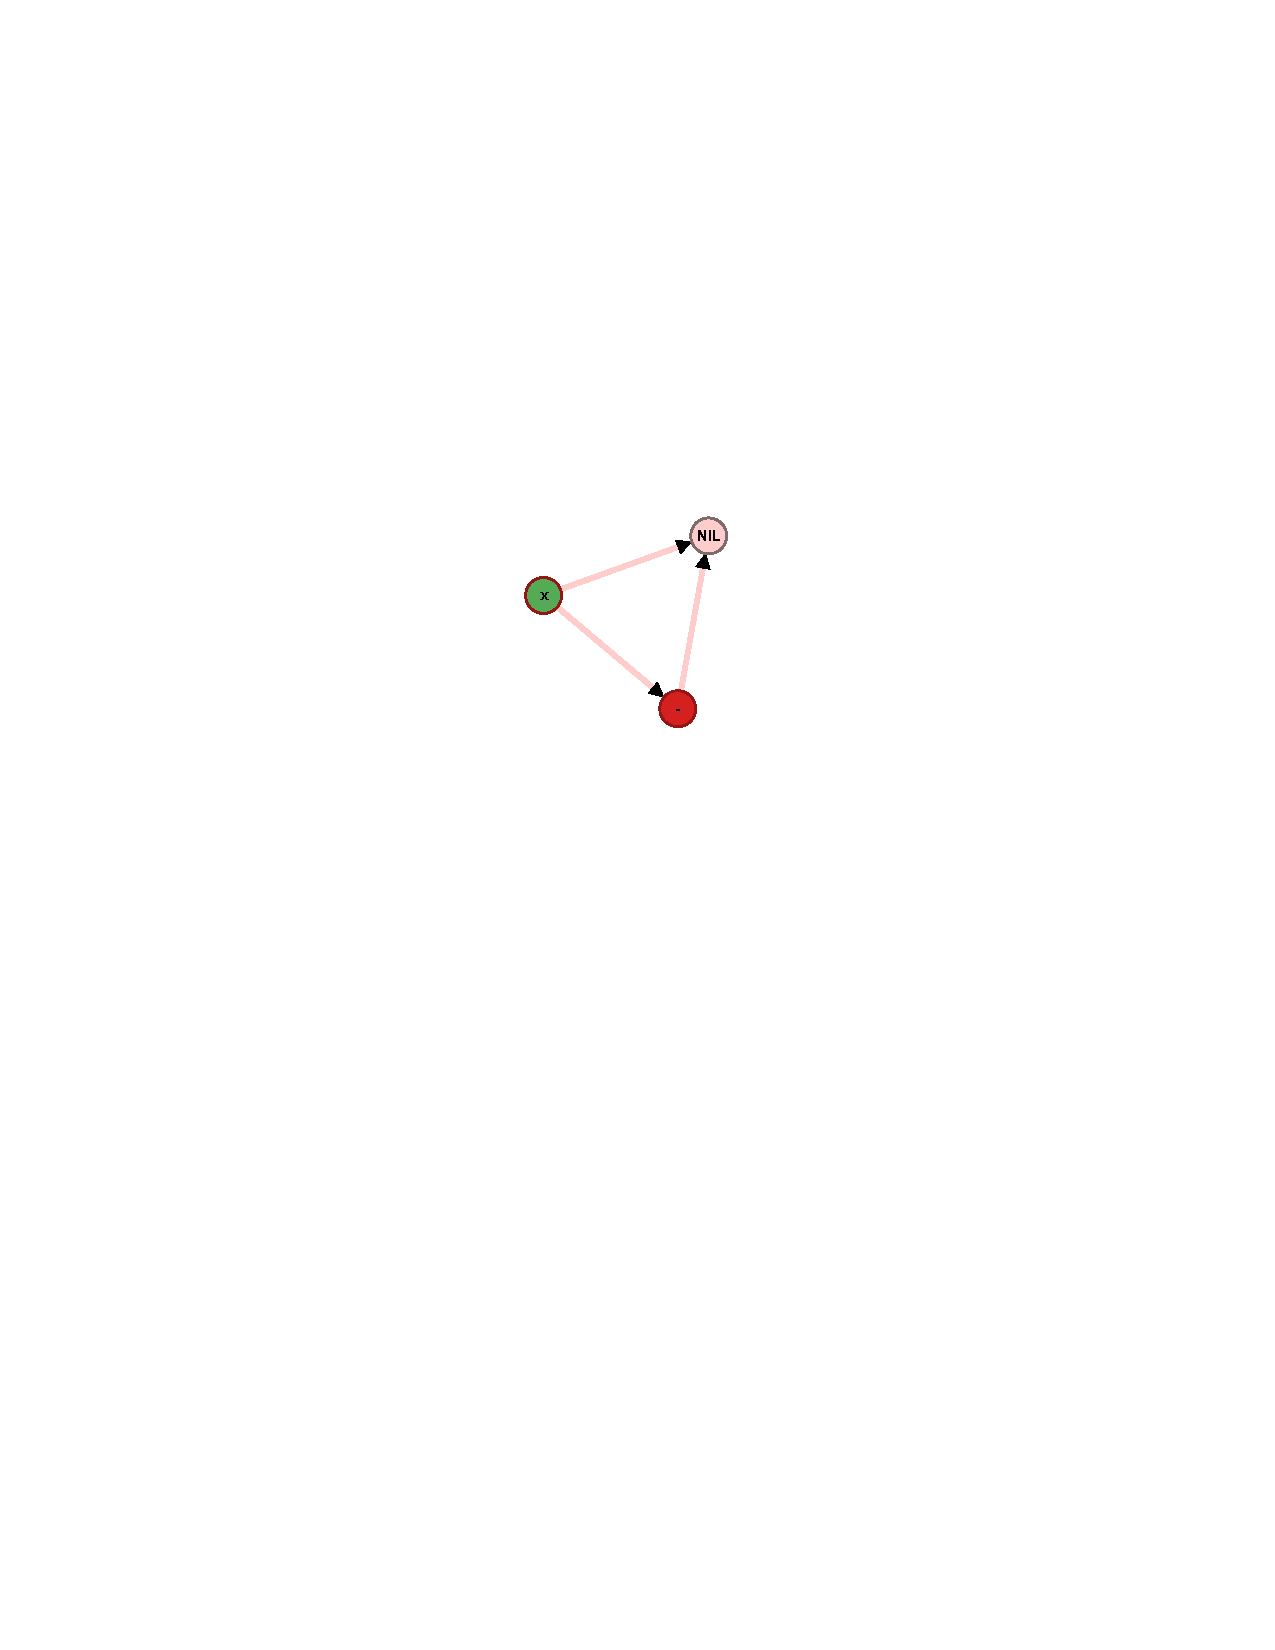
\includegraphics[width=7cm]{fig/candidate3.pdf}
  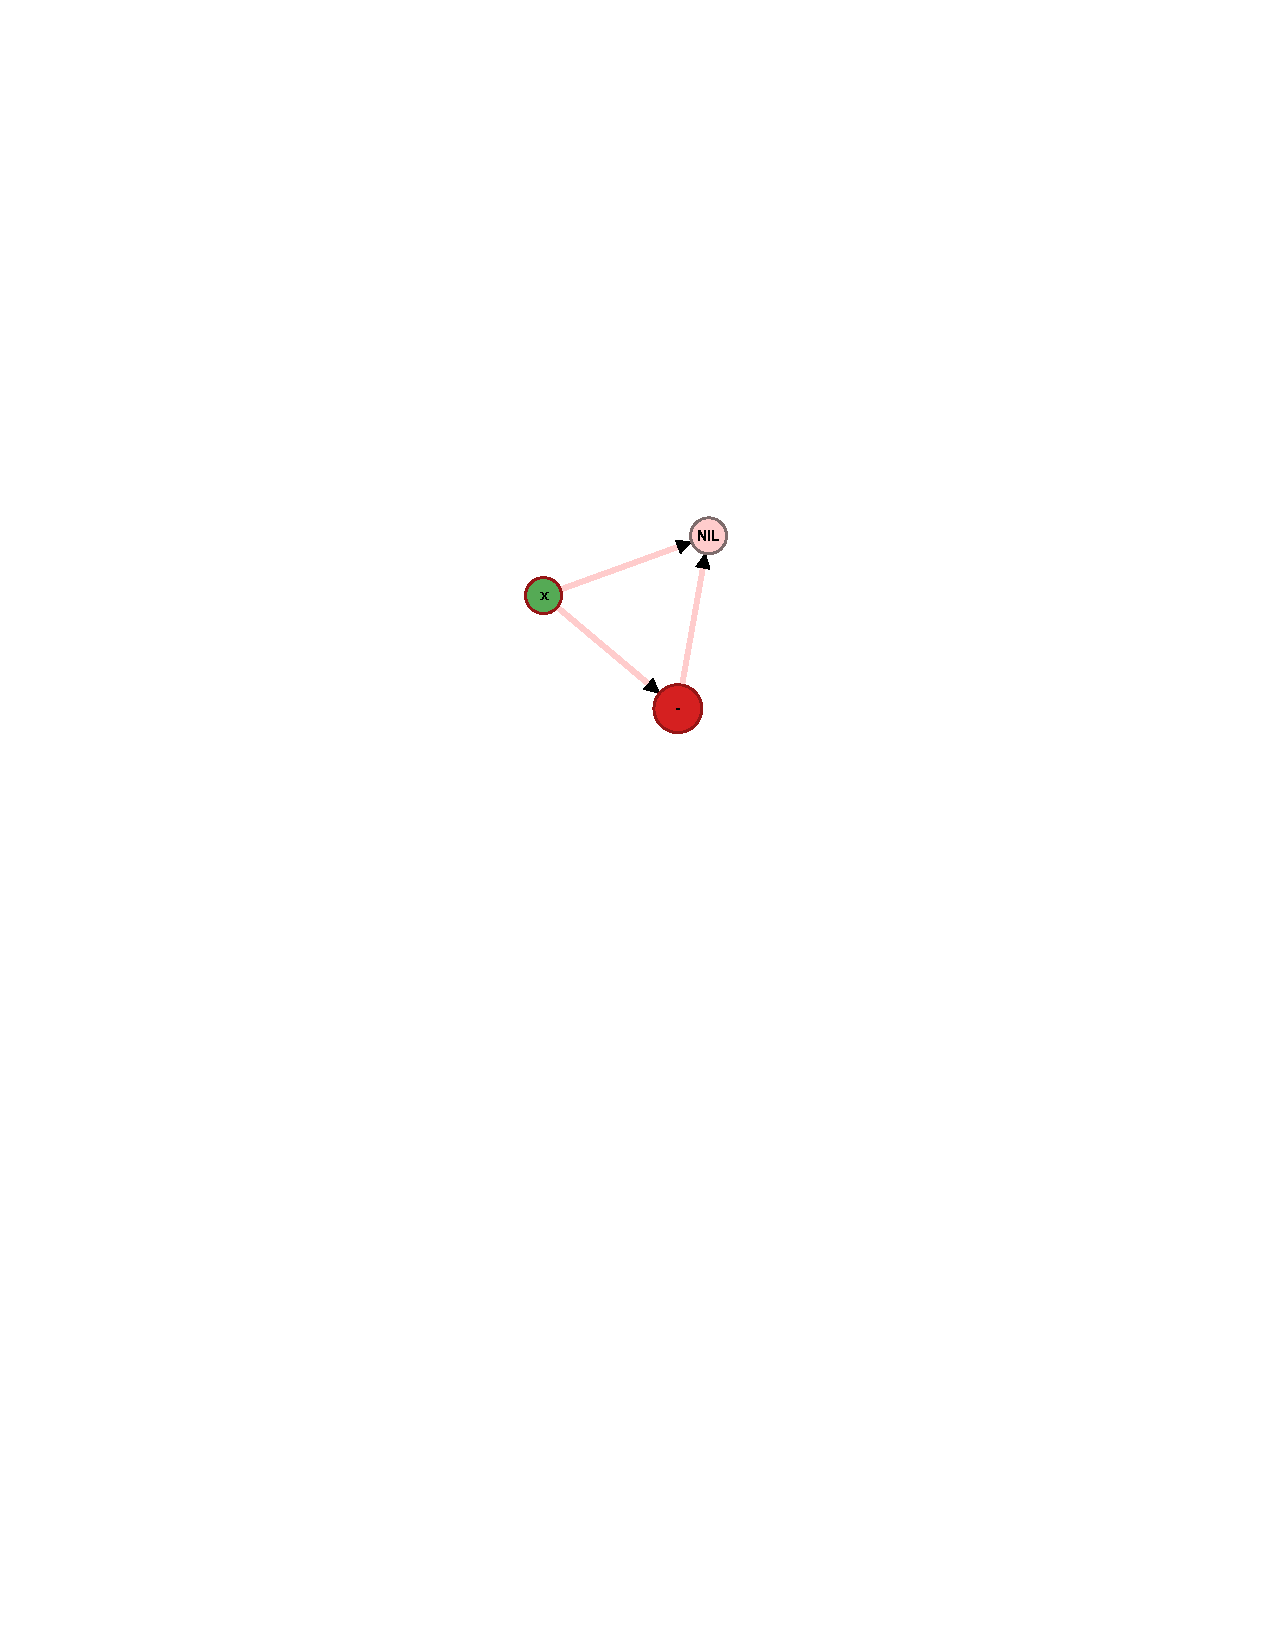
\includegraphics[width=7cm]{fig/candidate4.pdf}
  \caption{The user first provides the pattern on the left as a candidate. But we note that this pattern does not actually cover the first heap in $H^{+}$ in \autoref{fig:positive-examples}, so the interface highlights the first heap, and the user has to correct their input. After making one of the nodes a summary node (indicated by the larger size in the pattern on the right), the pattern starts to be entailed by both our heaps in $H^{+}$, and the interface passes it on to the verifier.}
  \label{fig:pattern-attempts}
\end{figure}

After several back and forth interactions with the verifier, we might end up in a state where we have several positive examples, as shown in in \autoref{fig:several-positive-examples}. The user now begins to get an idea of what the program might actually be doing at this program location. It looks like the program constructs ``alternating'' linked lists that always start with a node where the predicate is $\true$. The heap variable $x$ acts as the head of the list.

% Some positive examples.
\begin{figure}
  \centering
  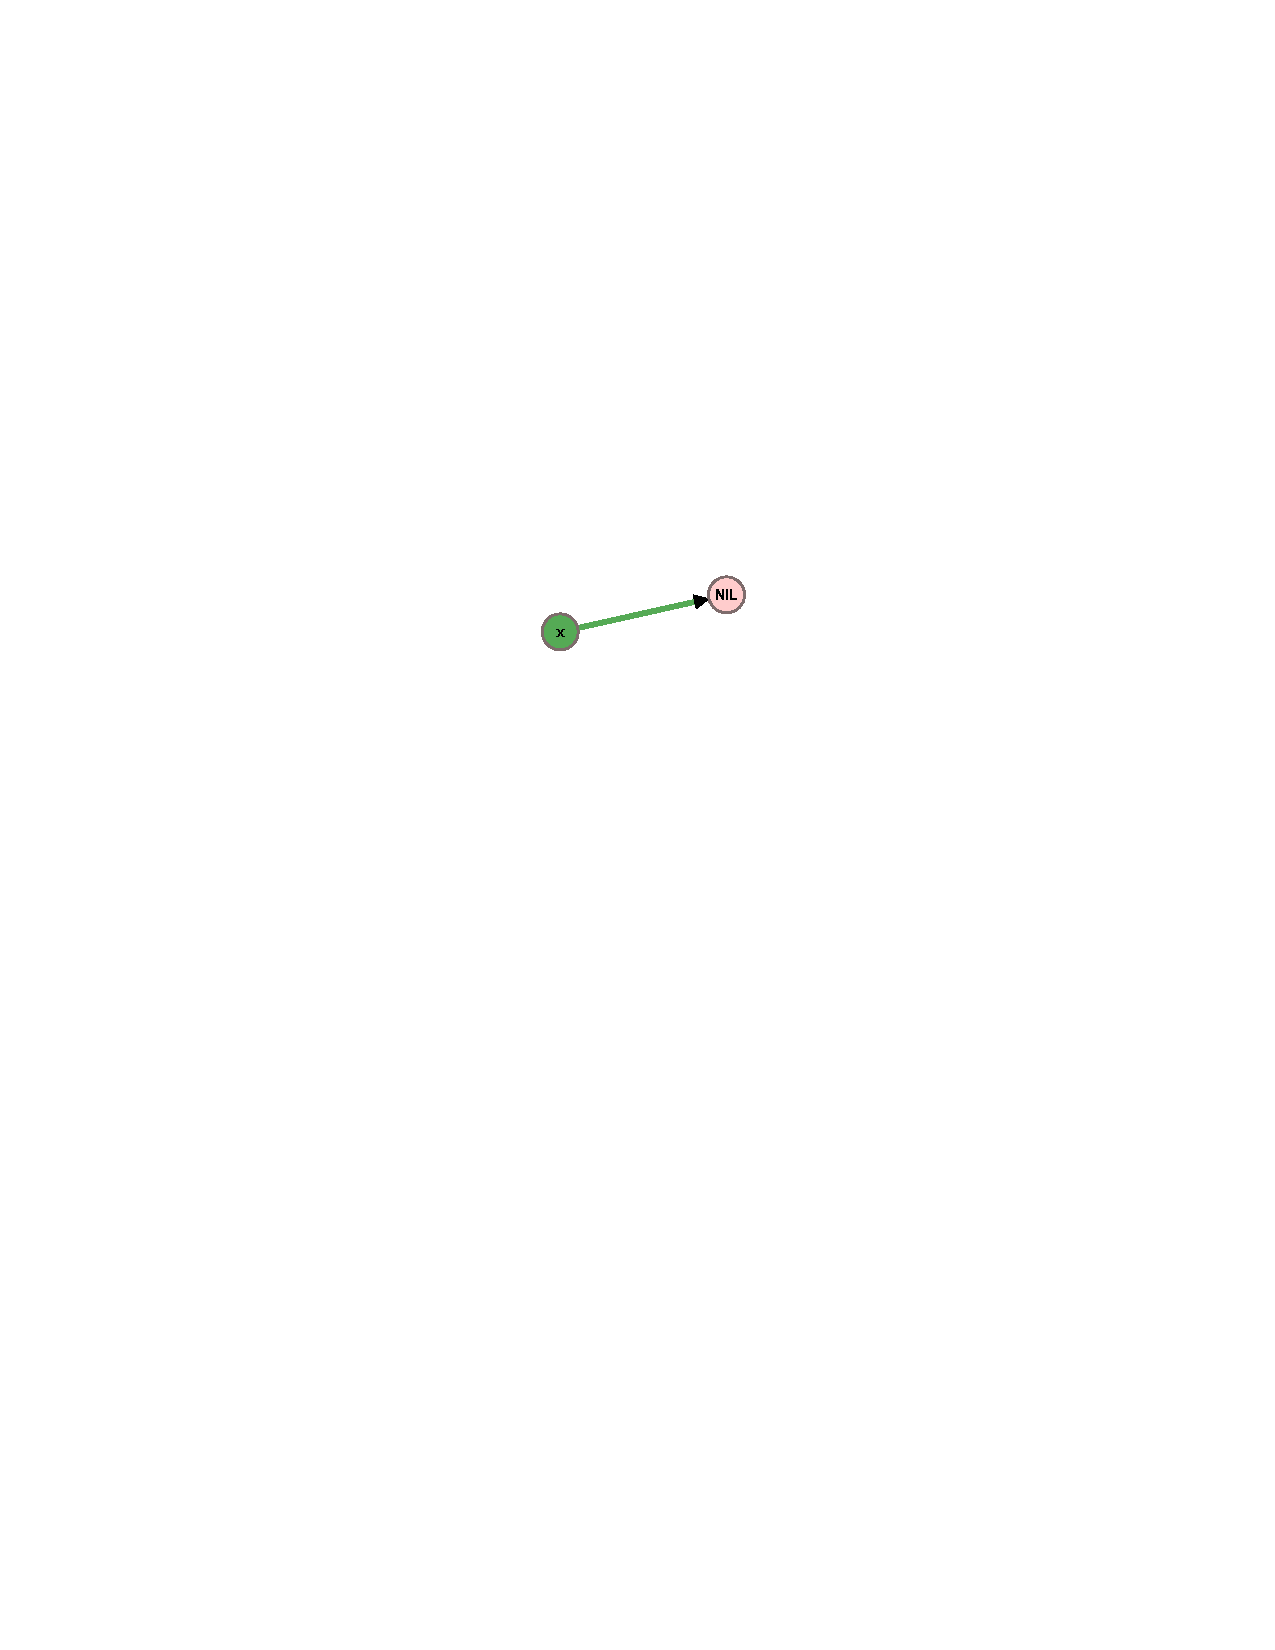
\includegraphics[width=5cm]{fig/positive1.pdf}
  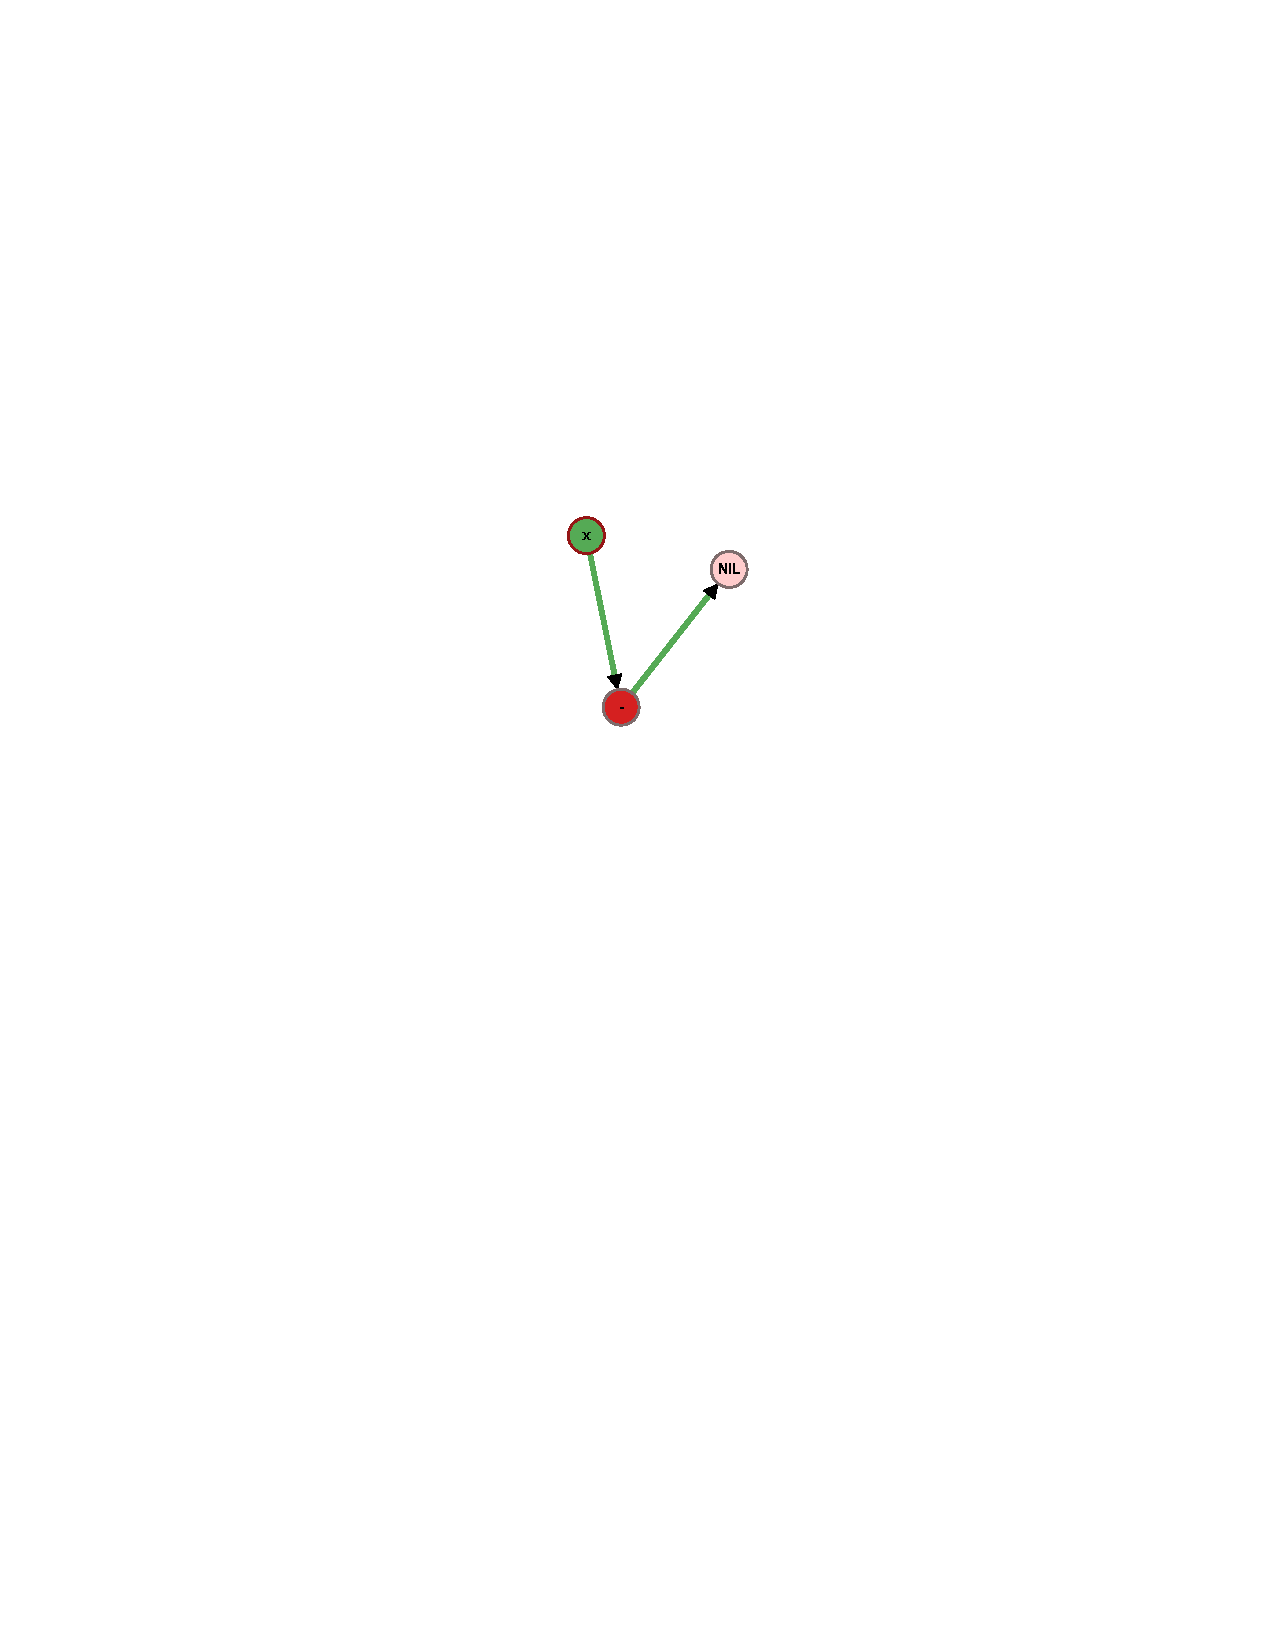
\includegraphics[width=5cm]{fig/positive2.pdf}
  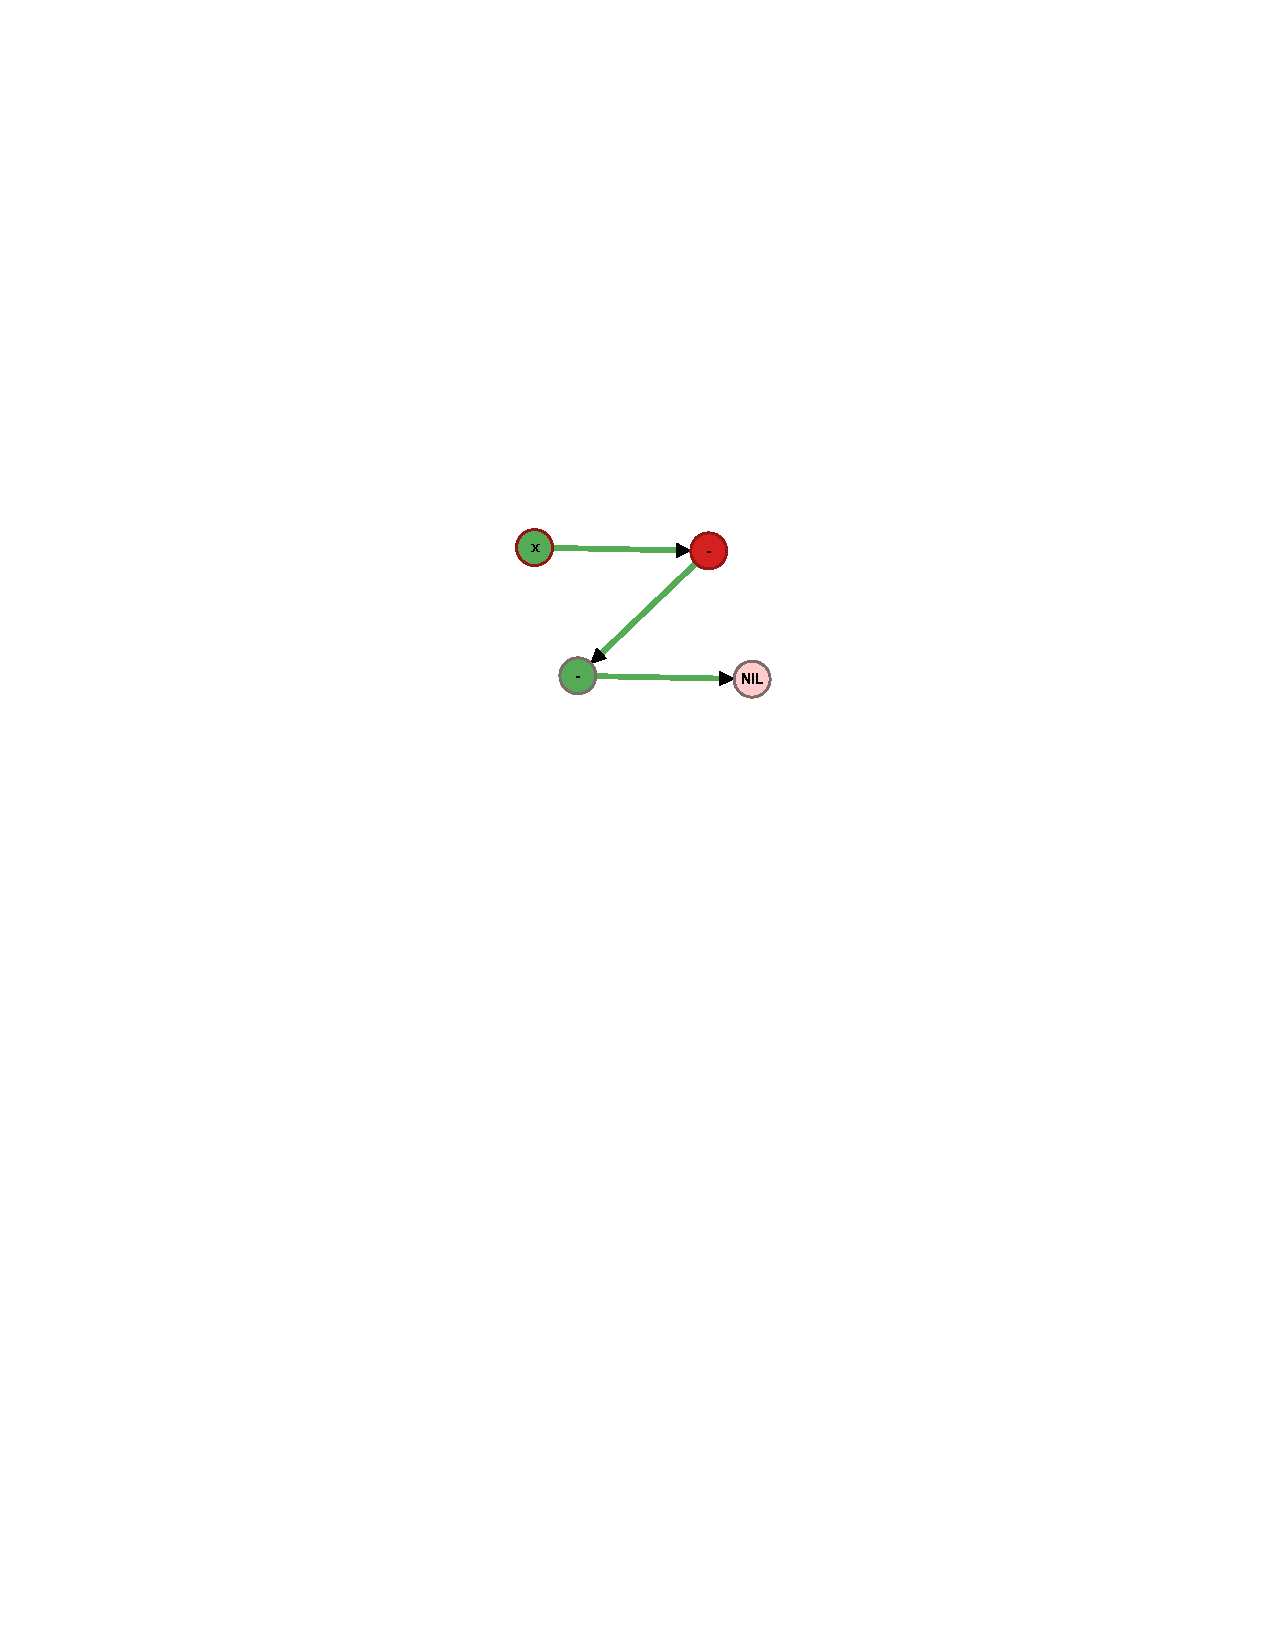
\includegraphics[width=5cm]{fig/positive3.pdf}
  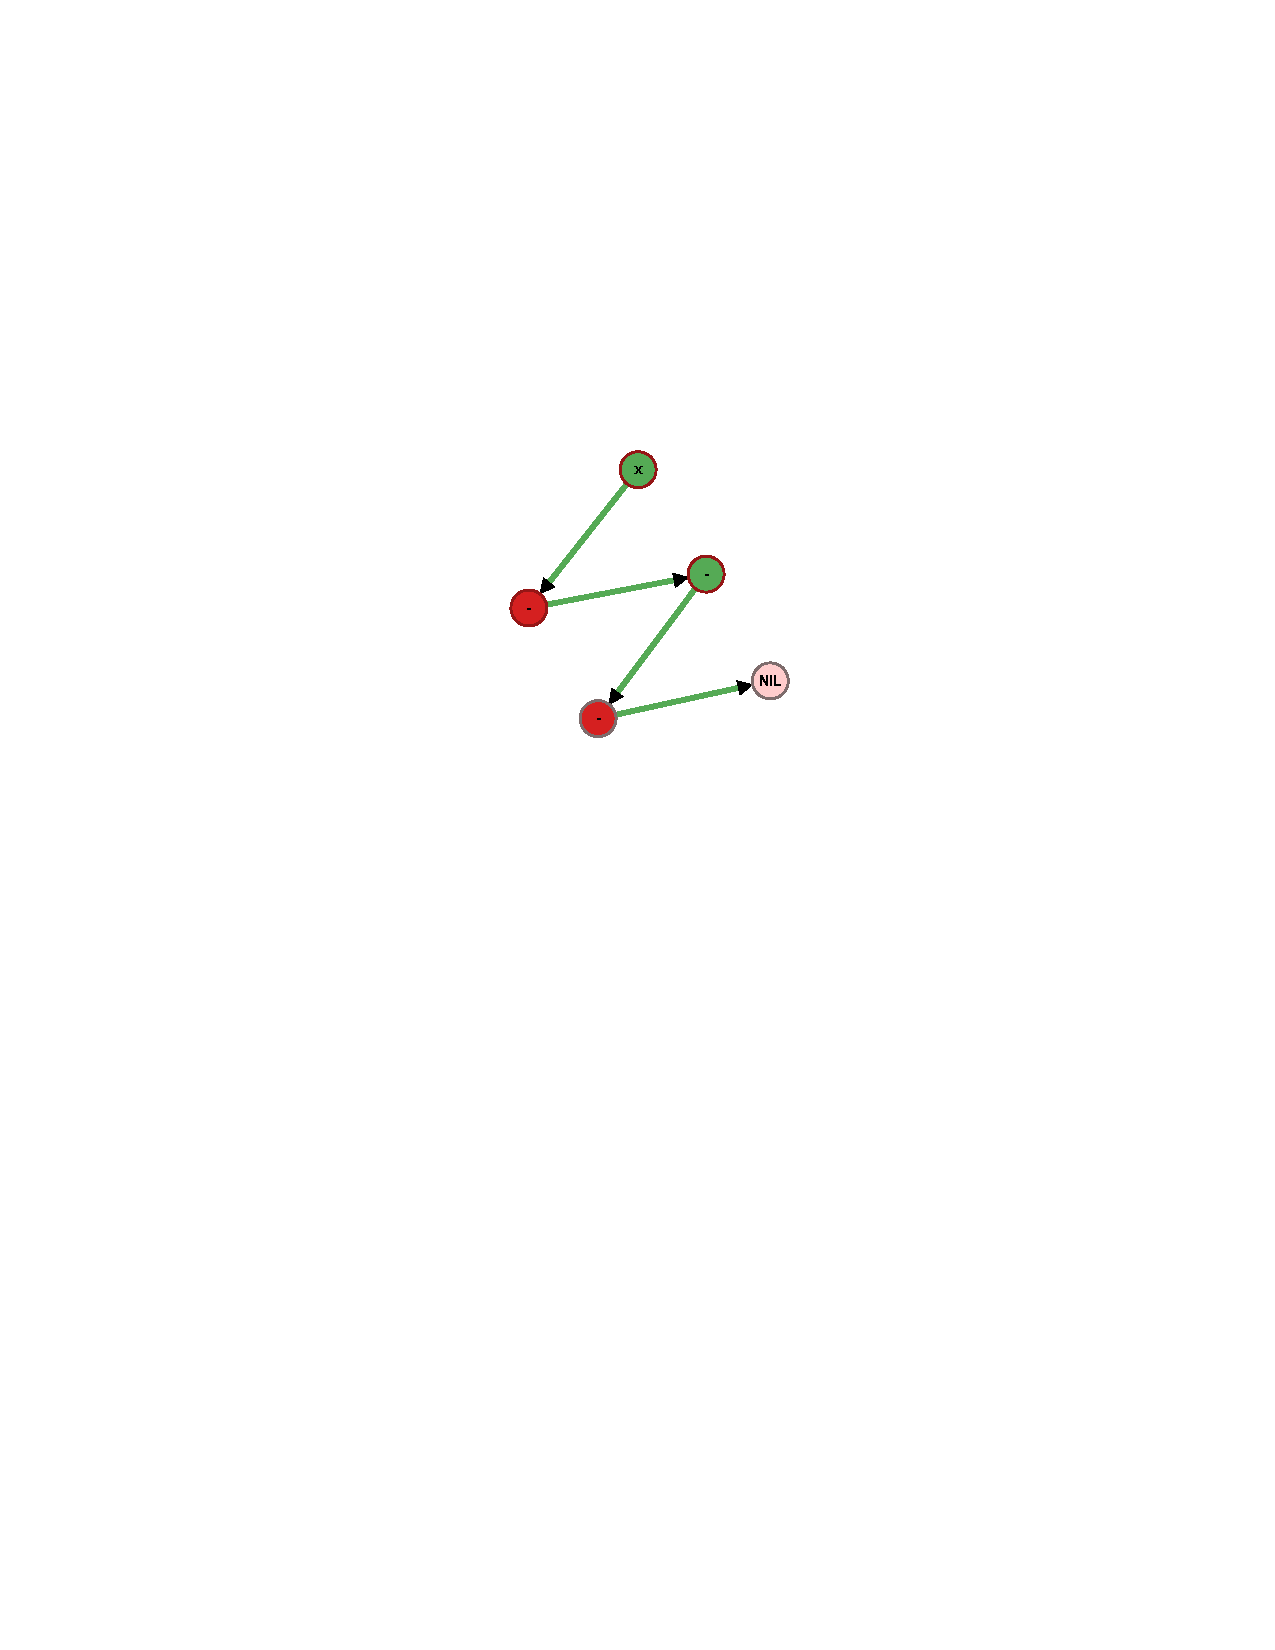
\includegraphics[width=5cm]{fig/positive4.pdf}
  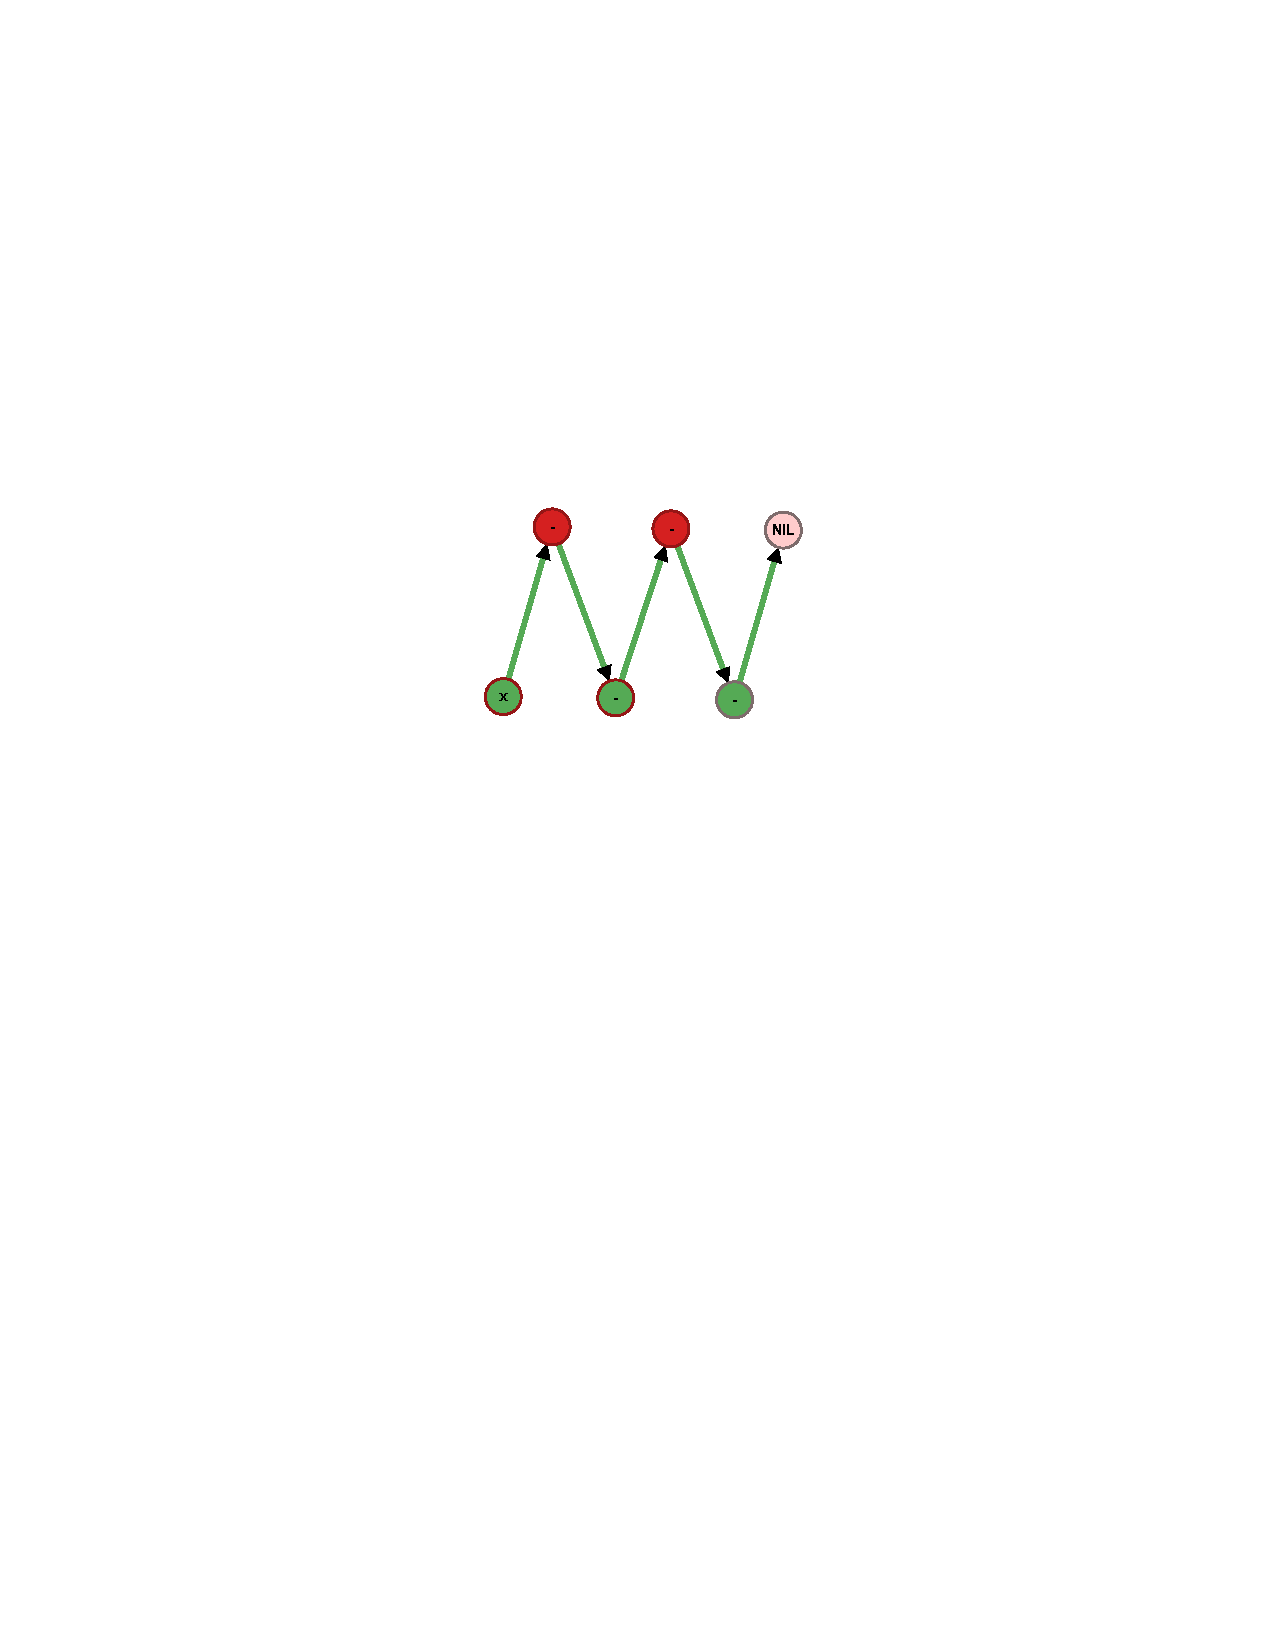
\includegraphics[width=5cm]{fig/positive5.pdf}
  \caption{The set $H^{+}$ of positive examples, after a few back and forth interactions between the user and the verifier. Note that a suitable candidate has still not been found, and $H^{-}$ is still empty.}
  \label{fig:several-positive-examples}
\end{figure}

After seeing all these examples, the user submits the pattern in \autoref{fig:almost-right-pattern}, hoping that it would be accepted by the verifier. It might well be, depending on what state the verifier is in. But in our example, the pattern provided by the user turns out to be too general, and the verifier returns a negative example for the first time. Finally, $H^{-}$ is non-empty, as looks as shown in \autoref{fig:negative-example}. Picking up on this, the user makes a correction, submitting the pattern in \autoref{fig:right-pattern}, which is finally accepted by the verifier.

% Almost right pattern.
\begin{figure}
  \centering
  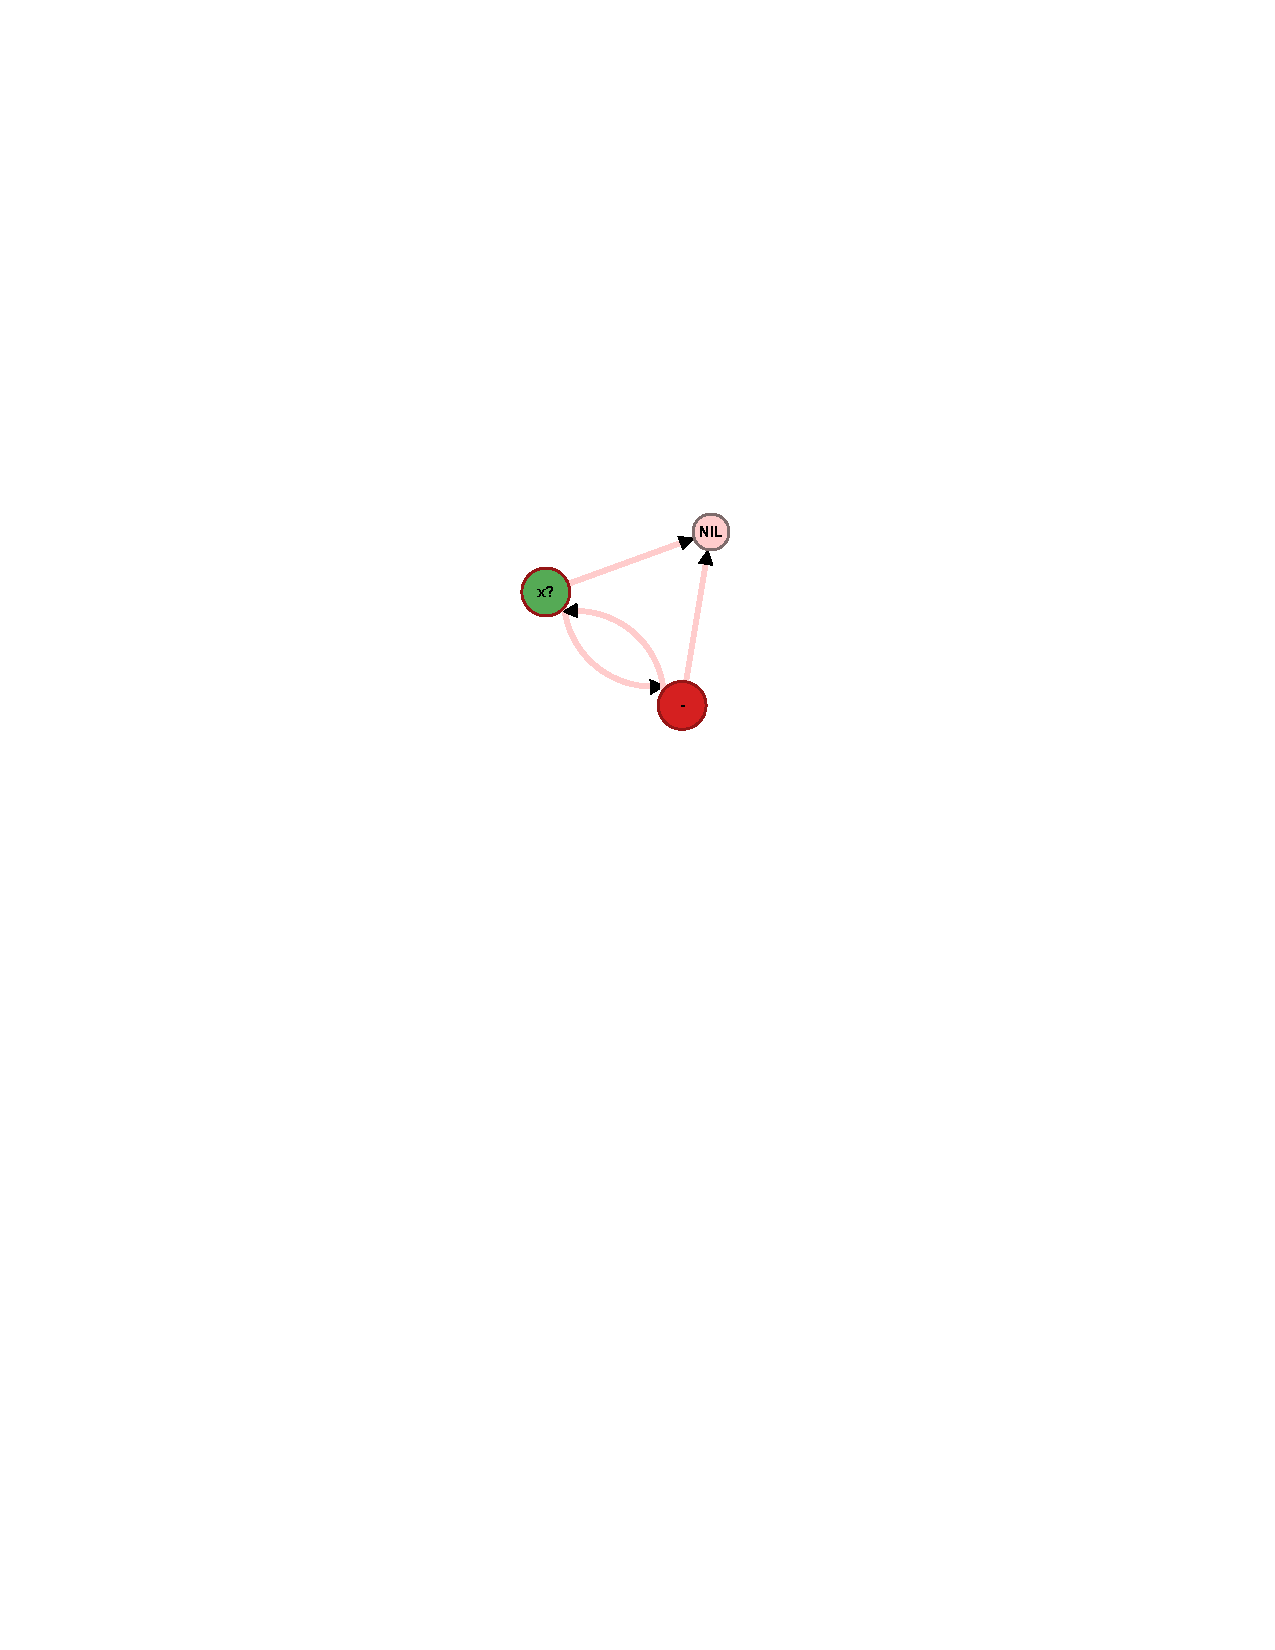
\includegraphics[width=7cm]{fig/candidate5.pdf}
  \caption{This candidate pattern is almost right, it captures the alternating list property, but has a problem that results in a negative example, shown in \autoref{fig:negative-example}.}
  \label{fig:almost-right-pattern}
\end{figure}

% Negative example.
\begin{figure}
  \centering
  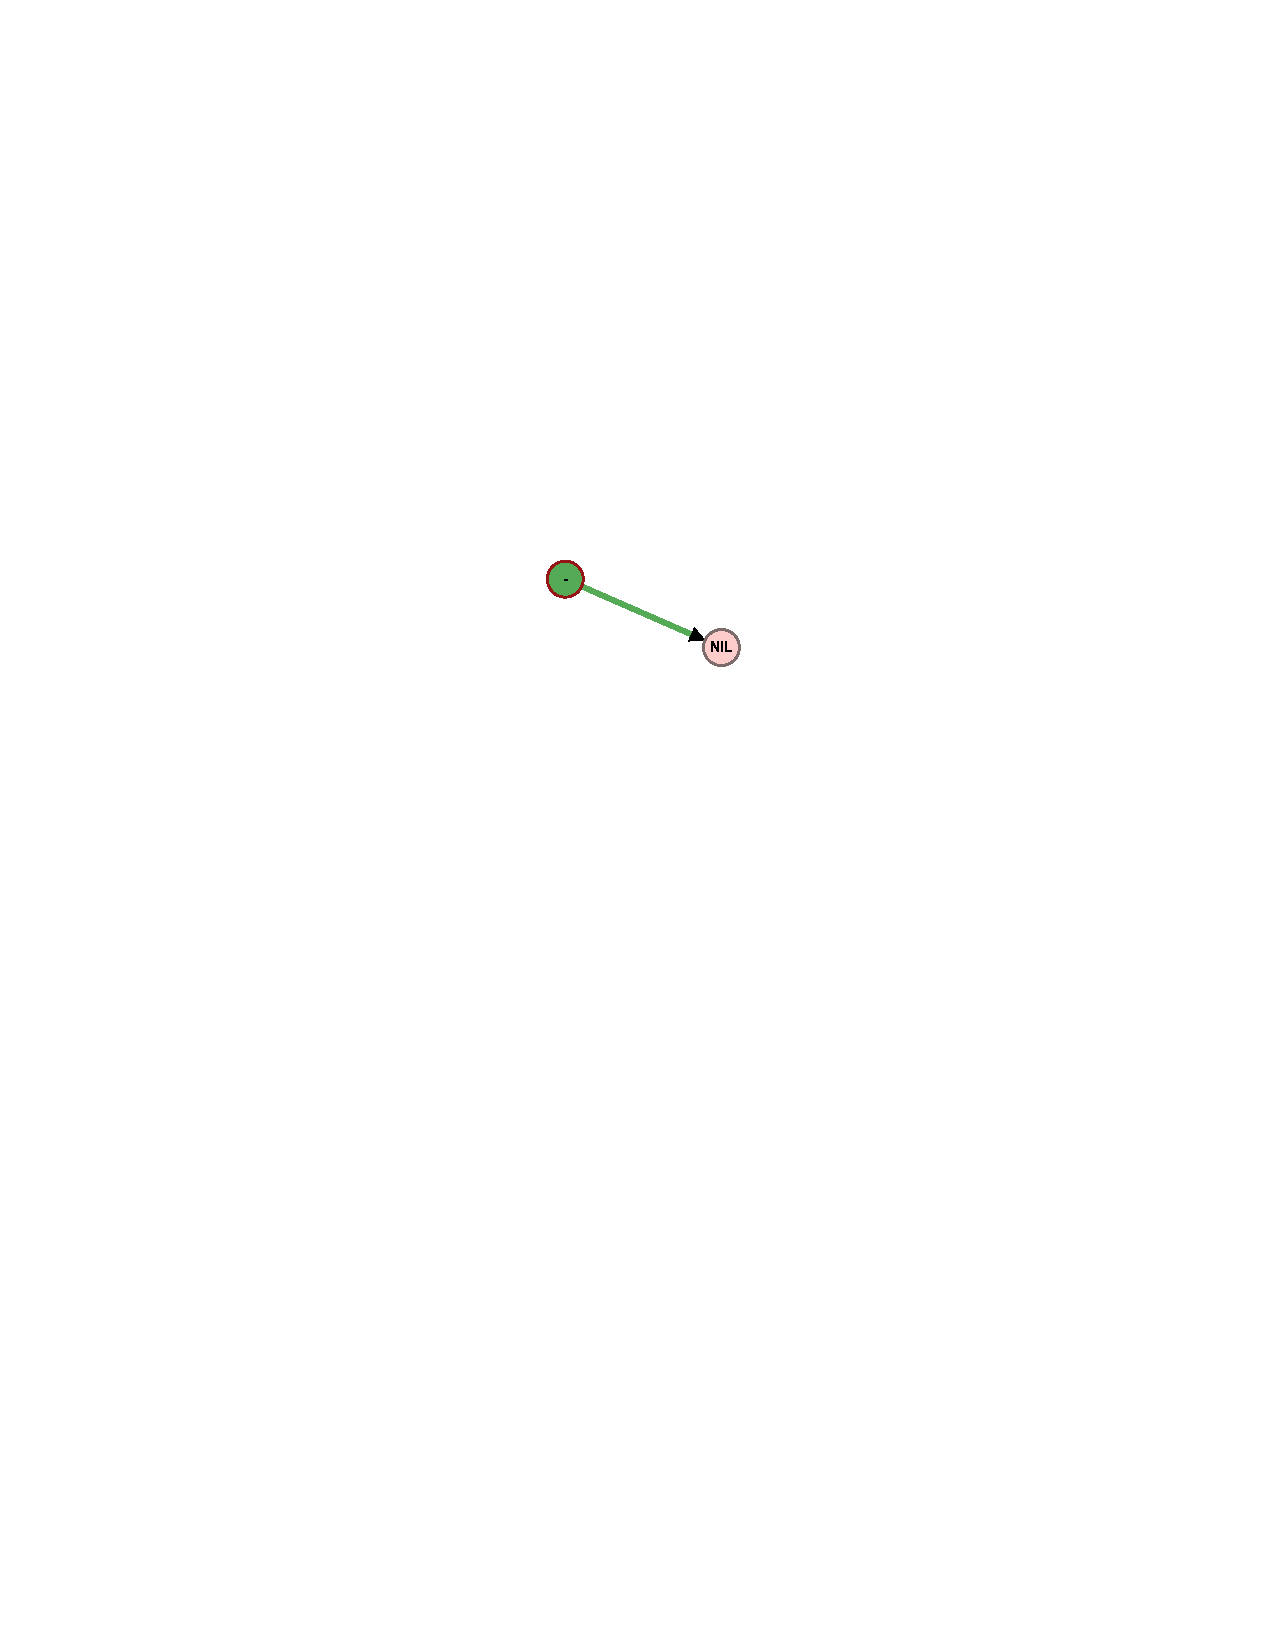
\includegraphics[width=7cm]{fig/negative1.pdf}
  \caption{The set $H^{-}$, with a simple heap that indicates that the first node does not have $x$ pointing to it. This heap is allowed by the pattern in \autoref{fig:almost-right-pattern}, but not by the pattern in \autoref{fig:right-pattern}.}
  \label{fig:negative-example}
\end{figure}

% Final right pattern.
\begin{figure}
  \centering
  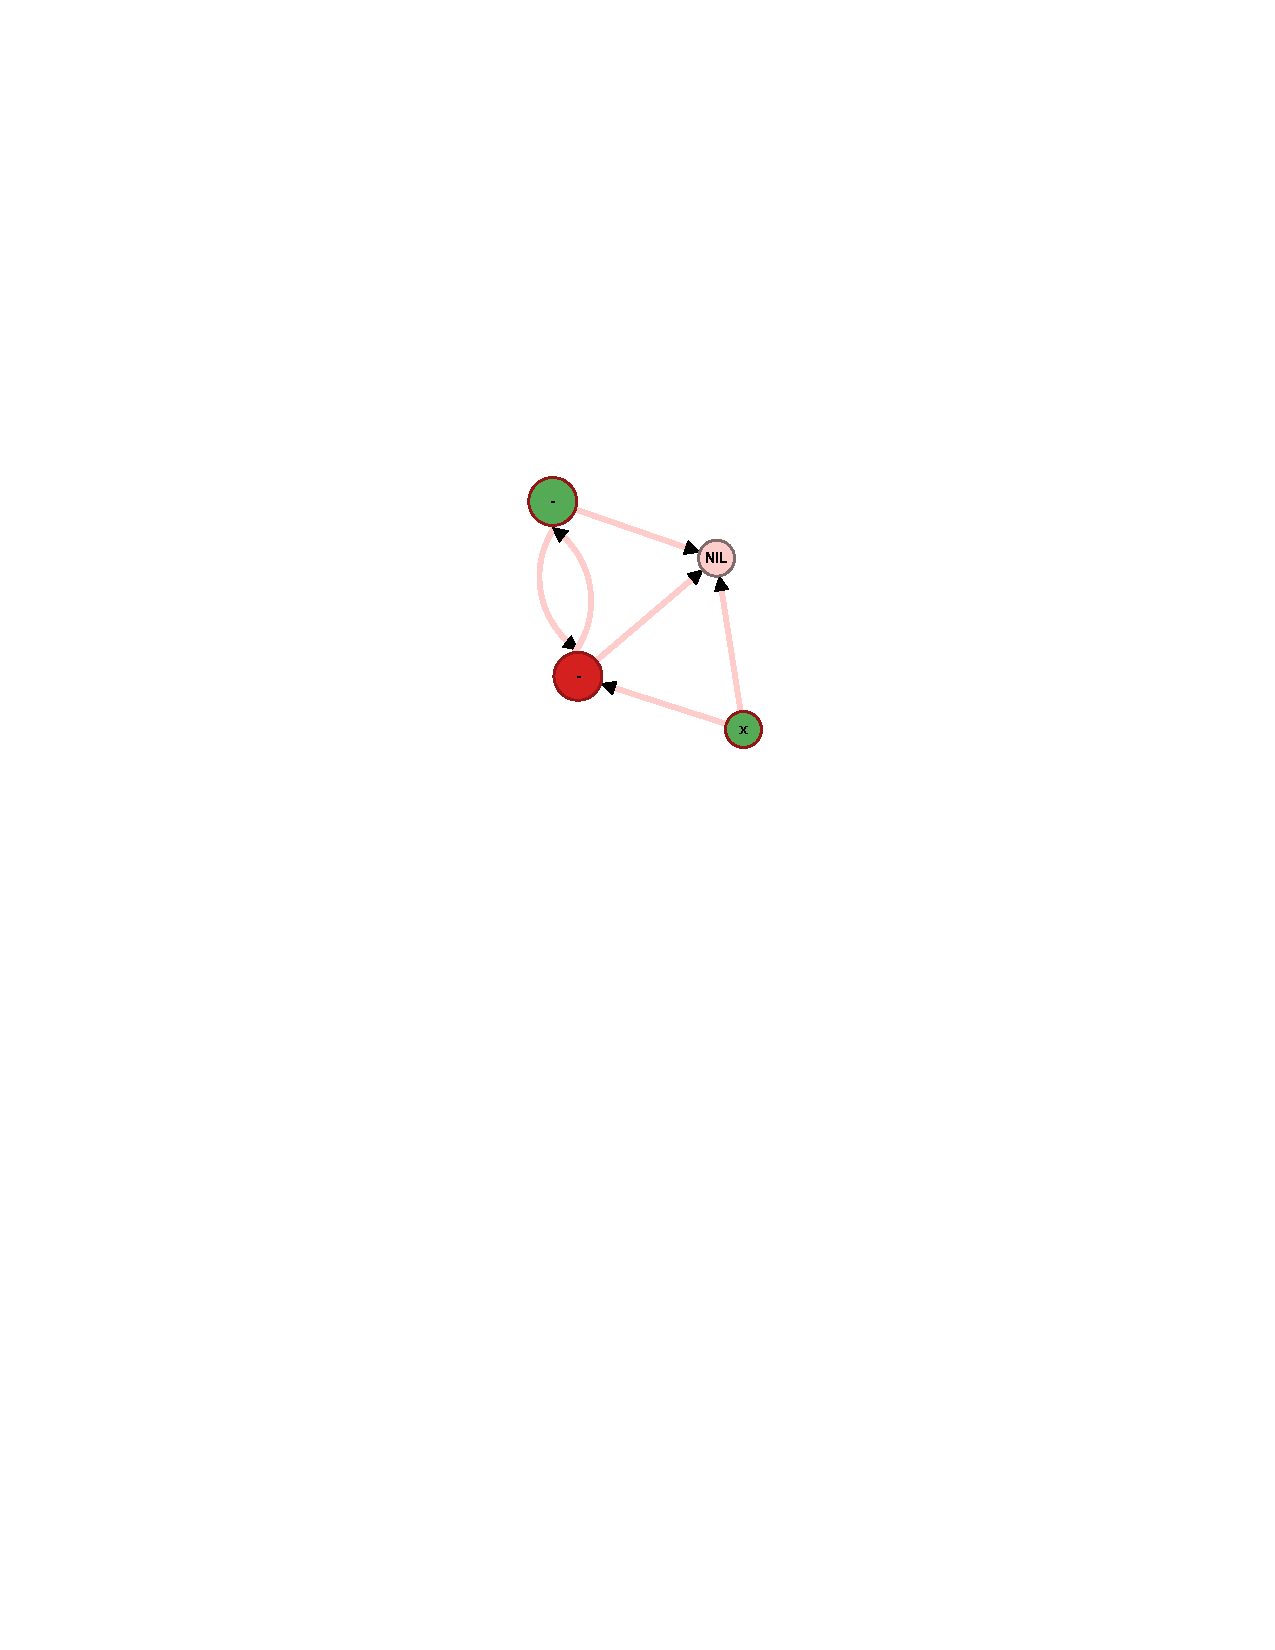
\includegraphics[width=7cm]{fig/candidate6.pdf}
  \caption{The final pattern that is accepted by the verifier. Note that this is not the strongest pattern indicating exactly the right heaps. \verifier does not need the strongest pattern, but the one that can be part of the interpolant. Too strong a pattern can lead to a lot of the vertices in the unwinding tree ending up uncovered. Too weak might mean the interpolant breaks down.}
  \label{fig:right-pattern}
\end{figure}

\section{Analyzing our Interface}
Our example in \autoref{sec:illustrating-user-interaction} gives one possible user interaction flow for the \altlistsimplified program, but our description would be incomplete without a broader discussion of the capabilities and limitations of our interface.

\subsection{Expressiveness of Heap Patterns}
\label{sec:expressiveness-of-heap-patterns}
Some visual examples of heap patterns depicting interesting properties. We don't yet have theoretical results for what class of examples can be expressed by our formalism, but that is future work. Besides, one of the points of demonstrating this is to show that different formalisms can be plugged in to play with expressiveness.

\subsection{Understandability of the Interface}
\label{sec:understandability-of-interface}
Describes the backgrounds of the users we asked to use it, and two examples for which they could work out reasonable patterns.

\subsection{Experiments}
Need better title for this section. Describe what exists in the implementation. (This is also part of Sanjit's feedback).

Also describe what needs to be done as future work.

\section*{Summary}
In this chapter, we presented the web interface for the Oracle in \verifier - a human user. We described the interface design, and an overview of how a user would interact with the interface to provide a useful heap pattern that can be used in verification. We also discussed our overall implementation and its limitations. The next chapter presents some related work, and concludes with  our contributions and ideas for potential directions to take.